\documentclass[twoside]{book}

% Packages required by doxygen
\usepackage{fixltx2e}
\usepackage{calc}
\usepackage{doxygen}
\usepackage[export]{adjustbox} % also loads graphicx
\usepackage{graphicx}
\usepackage[utf8]{inputenc}
\usepackage{makeidx}
\usepackage{multicol}
\usepackage{multirow}
\PassOptionsToPackage{warn}{textcomp}
\usepackage{textcomp}
\usepackage[nointegrals]{wasysym}
\usepackage[table]{xcolor}

% Font selection
\usepackage[T1]{fontenc}
\usepackage[scaled=.90]{helvet}
\usepackage{courier}
\usepackage{amssymb}
\usepackage{sectsty}
\renewcommand{\familydefault}{\sfdefault}
\allsectionsfont{%
  \fontseries{bc}\selectfont%
  \color{darkgray}%
}
\renewcommand{\DoxyLabelFont}{%
  \fontseries{bc}\selectfont%
  \color{darkgray}%
}
\newcommand{\+}{\discretionary{\mbox{\scriptsize$\hookleftarrow$}}{}{}}

% Page & text layout
\usepackage{geometry}
\geometry{%
  a4paper,%
  top=2.5cm,%
  bottom=2.5cm,%
  left=2.5cm,%
  right=2.5cm%
}
\tolerance=750
\hfuzz=15pt
\hbadness=750
\setlength{\emergencystretch}{15pt}
\setlength{\parindent}{0cm}
\setlength{\parskip}{3ex plus 2ex minus 2ex}
\makeatletter
\renewcommand{\paragraph}{%
  \@startsection{paragraph}{4}{0ex}{-1.0ex}{1.0ex}{%
    \normalfont\normalsize\bfseries\SS@parafont%
  }%
}
\renewcommand{\subparagraph}{%
  \@startsection{subparagraph}{5}{0ex}{-1.0ex}{1.0ex}{%
    \normalfont\normalsize\bfseries\SS@subparafont%
  }%
}
\makeatother

% Headers & footers
\usepackage{fancyhdr}
\pagestyle{fancyplain}
\fancyhead[LE]{\fancyplain{}{\bfseries\thepage}}
\fancyhead[CE]{\fancyplain{}{}}
\fancyhead[RE]{\fancyplain{}{\bfseries\leftmark}}
\fancyhead[LO]{\fancyplain{}{\bfseries\rightmark}}
\fancyhead[CO]{\fancyplain{}{}}
\fancyhead[RO]{\fancyplain{}{\bfseries\thepage}}
\fancyfoot[LE]{\fancyplain{}{}}
\fancyfoot[CE]{\fancyplain{}{}}
\fancyfoot[RE]{\fancyplain{}{\bfseries\scriptsize Generated by Doxygen }}
\fancyfoot[LO]{\fancyplain{}{\bfseries\scriptsize Generated by Doxygen }}
\fancyfoot[CO]{\fancyplain{}{}}
\fancyfoot[RO]{\fancyplain{}{}}
\renewcommand{\footrulewidth}{0.4pt}
\renewcommand{\chaptermark}[1]{%
  \markboth{#1}{}%
}
\renewcommand{\sectionmark}[1]{%
  \markright{\thesection\ #1}%
}

% Indices & bibliography
\usepackage{natbib}
\usepackage[titles]{tocloft}
\setcounter{tocdepth}{3}
\setcounter{secnumdepth}{5}
\makeindex

% Hyperlinks (required, but should be loaded last)
\usepackage{ifpdf}
\ifpdf
  \usepackage[pdftex,pagebackref=true]{hyperref}
\else
  \usepackage[ps2pdf,pagebackref=true]{hyperref}
\fi
\hypersetup{%
  colorlinks=true,%
  linkcolor=blue,%
  citecolor=blue,%
  unicode%
}

% Custom commands
\newcommand{\clearemptydoublepage}{%
  \newpage{\pagestyle{empty}\cleardoublepage}%
}

\usepackage{caption}
\captionsetup{labelsep=space,justification=centering,font={bf},singlelinecheck=off,skip=4pt,position=top}

%===== C O N T E N T S =====

\begin{document}

% Titlepage & ToC
\hypersetup{pageanchor=false,
             bookmarksnumbered=true,
             pdfencoding=unicode
            }
\pagenumbering{roman}
\begin{titlepage}
\vspace*{7cm}
\begin{center}%
{\Large Space\+Pig\+Fighter \\[1ex]\large 1.\+5 }\\
\vspace*{1cm}
{\large Generated by Doxygen 1.8.11}\\
\end{center}
\end{titlepage}
\clearemptydoublepage
\tableofcontents
\clearemptydoublepage
\pagenumbering{arabic}
\hypersetup{pageanchor=true}

%--- Begin generated contents ---
\chapter{Hierarchical Index}
\section{Class Hierarchy}
This inheritance list is sorted roughly, but not completely, alphabetically\+:\begin{DoxyCompactList}
\item \contentsline{section}{animal\+Package.\+Animal}{\pageref{classanimal_package_1_1_animal}}{}
\begin{DoxyCompactList}
\item \contentsline{section}{animal\+Package.\+With\+Paws}{\pageref{classanimal_package_1_1_with_paws}}{}
\begin{DoxyCompactList}
\item \contentsline{section}{animal\+Package.\+Bear}{\pageref{classanimal_package_1_1_bear}}{}
\item \contentsline{section}{animal\+Package.\+Pig}{\pageref{classanimal_package_1_1_pig}}{}
\item \contentsline{section}{animal\+Package.\+Tiger}{\pageref{classanimal_package_1_1_tiger}}{}
\end{DoxyCompactList}
\item \contentsline{section}{animal\+Package.\+With\+Wings}{\pageref{classanimal_package_1_1_with_wings}}{}
\begin{DoxyCompactList}
\item \contentsline{section}{animal\+Package.\+Chicken}{\pageref{classanimal_package_1_1_chicken}}{}
\item \contentsline{section}{animal\+Package.\+Duck}{\pageref{classanimal_package_1_1_duck}}{}
\end{DoxyCompactList}
\end{DoxyCompactList}
\item \contentsline{section}{animal\+Package.\+Be\+Fierce}{\pageref{interfaceanimal_package_1_1_be_fierce}}{}
\begin{DoxyCompactList}
\item \contentsline{section}{animal\+Package.\+Bear}{\pageref{classanimal_package_1_1_bear}}{}
\item \contentsline{section}{animal\+Package.\+Chicken}{\pageref{classanimal_package_1_1_chicken}}{}
\item \contentsline{section}{animal\+Package.\+Tiger}{\pageref{classanimal_package_1_1_tiger}}{}
\end{DoxyCompactList}
\item \contentsline{section}{cube\+Environment.\+Cube\+Environment}{\pageref{classcube_environment_1_1_cube_environment}}{}
\item \contentsline{section}{stuff.\+Defensif}{\pageref{classstuff_1_1_defensif}}{}
\item Exception\begin{DoxyCompactList}
\item \contentsline{section}{space\+Objects.\+Position\+Exception}{\pageref{classspace_objects_1_1_position_exception}}{}
\end{DoxyCompactList}
\item \contentsline{section}{space\+Pig\+Fighter\+Package.\+Execution\+Interface}{\pageref{interfacespace_pig_fighter_package_1_1_execution_interface}}{}
\begin{DoxyCompactList}
\item \contentsline{section}{space\+Pig\+Fighter\+Package.\+Fight\+Area}{\pageref{classspace_pig_fighter_package_1_1_fight_area}}{}
\item \contentsline{section}{space\+Pig\+Fighter\+Package.\+Space}{\pageref{classspace_pig_fighter_package_1_1_space}}{}
\end{DoxyCompactList}
\item \contentsline{section}{file\+Management\+Package.\+File\+Management}{\pageref{classfile_management_package_1_1_file_management}}{}
\item \contentsline{section}{space\+Pig\+Fighter\+Package.\+Main}{\pageref{classspace_pig_fighter_package_1_1_main}}{}
\item \contentsline{section}{space\+Objects.\+Meteorite\+Size}{\pageref{enumspace_objects_1_1_meteorite_size}}{}
\item \contentsline{section}{stuff.\+Offensif}{\pageref{classstuff_1_1_offensif}}{}
\item \contentsline{section}{player\+Package.\+Player}{\pageref{classplayer_package_1_1_player}}{}
\item \contentsline{section}{space\+Objects.\+Positions\+Cube}{\pageref{enumspace_objects_1_1_positions_cube}}{}
\item \contentsline{section}{space\+Objects.\+Ufo}{\pageref{classspace_objects_1_1_ufo}}{}
\begin{DoxyCompactList}
\item \contentsline{section}{space\+Objects.\+Meteorite}{\pageref{classspace_objects_1_1_meteorite}}{}
\item \contentsline{section}{space\+Objects.\+Spacecraft}{\pageref{classspace_objects_1_1_spacecraft}}{}
\end{DoxyCompactList}
\end{DoxyCompactList}

\chapter{Class Index}
\section{Class List}
Here are the classes, structs, unions and interfaces with brief descriptions\+:\begin{DoxyCompactList}
\item\contentsline{section}{\hyperlink{classanimal_package_1_1_animal}{animal\+Package.\+Animal} }{\pageref{classanimal_package_1_1_animal}}{}
\item\contentsline{section}{\hyperlink{classanimal_package_1_1_bear}{animal\+Package.\+Bear} }{\pageref{classanimal_package_1_1_bear}}{}
\item\contentsline{section}{\hyperlink{interfaceanimal_package_1_1_be_fierce}{animal\+Package.\+Be\+Fierce} }{\pageref{interfaceanimal_package_1_1_be_fierce}}{}
\item\contentsline{section}{\hyperlink{classanimal_package_1_1_chicken}{animal\+Package.\+Chicken} }{\pageref{classanimal_package_1_1_chicken}}{}
\item\contentsline{section}{\hyperlink{classcube_environment_1_1_cube_environment}{cube\+Environment.\+Cube\+Environment} }{\pageref{classcube_environment_1_1_cube_environment}}{}
\item\contentsline{section}{\hyperlink{classstuff_1_1_defensif}{stuff.\+Defensif} }{\pageref{classstuff_1_1_defensif}}{}
\item\contentsline{section}{\hyperlink{classanimal_package_1_1_duck}{animal\+Package.\+Duck} }{\pageref{classanimal_package_1_1_duck}}{}
\item\contentsline{section}{\hyperlink{interfacespace_pig_fighter_package_1_1_execution_interface}{space\+Pig\+Fighter\+Package.\+Execution\+Interface} }{\pageref{interfacespace_pig_fighter_package_1_1_execution_interface}}{}
\item\contentsline{section}{\hyperlink{classspace_pig_fighter_package_1_1_fight_area}{space\+Pig\+Fighter\+Package.\+Fight\+Area} }{\pageref{classspace_pig_fighter_package_1_1_fight_area}}{}
\item\contentsline{section}{\hyperlink{classfile_management_package_1_1_file_management}{file\+Management\+Package.\+File\+Management} }{\pageref{classfile_management_package_1_1_file_management}}{}
\item\contentsline{section}{\hyperlink{classspace_pig_fighter_package_1_1_main}{space\+Pig\+Fighter\+Package.\+Main} }{\pageref{classspace_pig_fighter_package_1_1_main}}{}
\item\contentsline{section}{\hyperlink{classspace_objects_1_1_meteorite}{space\+Objects.\+Meteorite} }{\pageref{classspace_objects_1_1_meteorite}}{}
\item\contentsline{section}{\hyperlink{enumspace_objects_1_1_meteorite_size}{space\+Objects.\+Meteorite\+Size} }{\pageref{enumspace_objects_1_1_meteorite_size}}{}
\item\contentsline{section}{\hyperlink{classstuff_1_1_offensif}{stuff.\+Offensif} }{\pageref{classstuff_1_1_offensif}}{}
\item\contentsline{section}{\hyperlink{classanimal_package_1_1_pig}{animal\+Package.\+Pig} }{\pageref{classanimal_package_1_1_pig}}{}
\item\contentsline{section}{\hyperlink{classplayer_package_1_1_player}{player\+Package.\+Player} }{\pageref{classplayer_package_1_1_player}}{}
\item\contentsline{section}{\hyperlink{classspace_objects_1_1_position_exception}{space\+Objects.\+Position\+Exception} }{\pageref{classspace_objects_1_1_position_exception}}{}
\item\contentsline{section}{\hyperlink{enumspace_objects_1_1_positions_cube}{space\+Objects.\+Positions\+Cube} }{\pageref{enumspace_objects_1_1_positions_cube}}{}
\item\contentsline{section}{\hyperlink{classspace_pig_fighter_package_1_1_space}{space\+Pig\+Fighter\+Package.\+Space} }{\pageref{classspace_pig_fighter_package_1_1_space}}{}
\item\contentsline{section}{\hyperlink{classspace_objects_1_1_spacecraft}{space\+Objects.\+Spacecraft} }{\pageref{classspace_objects_1_1_spacecraft}}{}
\item\contentsline{section}{\hyperlink{classanimal_package_1_1_tiger}{animal\+Package.\+Tiger} }{\pageref{classanimal_package_1_1_tiger}}{}
\item\contentsline{section}{\hyperlink{classspace_objects_1_1_ufo}{space\+Objects.\+Ufo} }{\pageref{classspace_objects_1_1_ufo}}{}
\item\contentsline{section}{\hyperlink{classanimal_package_1_1_with_paws}{animal\+Package.\+With\+Paws} }{\pageref{classanimal_package_1_1_with_paws}}{}
\item\contentsline{section}{\hyperlink{classanimal_package_1_1_with_wings}{animal\+Package.\+With\+Wings} }{\pageref{classanimal_package_1_1_with_wings}}{}
\end{DoxyCompactList}

\chapter{Class Documentation}
\hypertarget{classanimal_package_1_1_animal}{}\section{animal\+Package.\+Animal Class Reference}
\label{classanimal_package_1_1_animal}\index{animal\+Package.\+Animal@{animal\+Package.\+Animal}}


Inheritance diagram for animal\+Package.\+Animal\+:\nopagebreak
\begin{figure}[H]
\begin{center}
\leavevmode
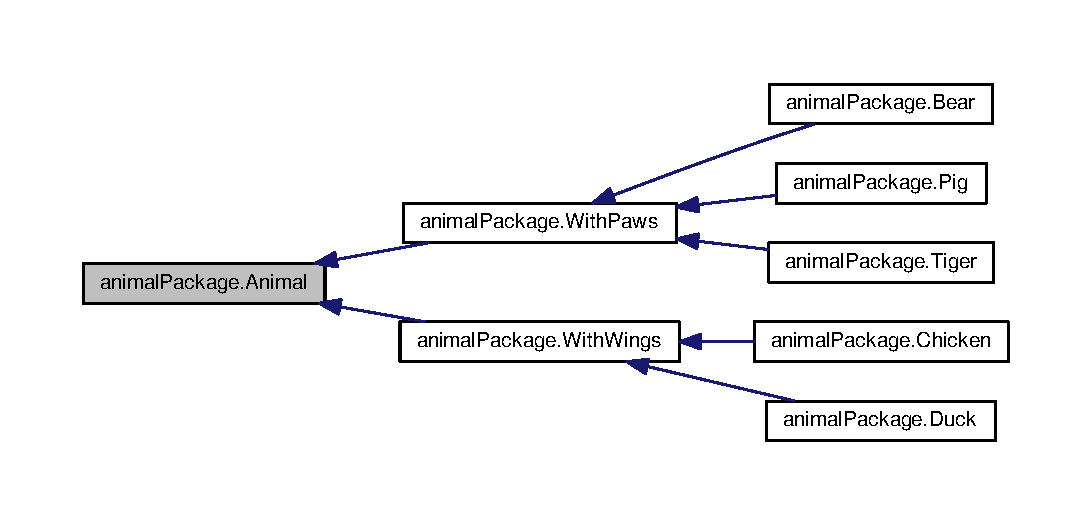
\includegraphics[width=350pt]{classanimal_package_1_1_animal__inherit__graph}
\end{center}
\end{figure}


Collaboration diagram for animal\+Package.\+Animal\+:\nopagebreak
\begin{figure}[H]
\begin{center}
\leavevmode
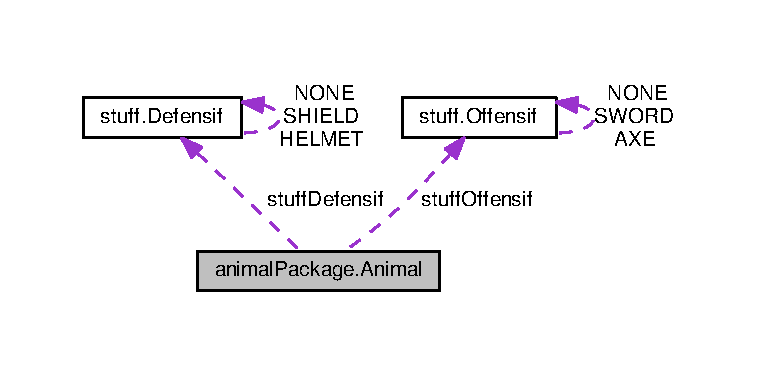
\includegraphics[width=350pt]{classanimal_package_1_1_animal__coll__graph}
\end{center}
\end{figure}
\subsection*{Public Member Functions}
\begin{DoxyCompactItemize}
\item 
\hyperlink{classanimal_package_1_1_animal_af9ac4bd4d9d42913ffdf51a03d590b44}{Animal} (String new\+Pseudo)
\item 
\hyperlink{classanimal_package_1_1_animal_a7297a8c17c12bb30e0696da4f6087226}{Animal} (String new\+Pseudo, String new\+Color)
\item 
String \hyperlink{classanimal_package_1_1_animal_a15510acce4c89705599c66895d5794cc}{get\+Color} ()
\item 
Integer \hyperlink{classanimal_package_1_1_animal_aaec6fd7842858e7e68f4928639068ca7}{get\+Force} ()
\item 
Integer \hyperlink{classanimal_package_1_1_animal_a5aa0361400091f06e398d84e12941a09}{get\+Life} ()
\item 
String \hyperlink{classanimal_package_1_1_animal_af0394bd0a44e024fe043a20d73331be4}{get\+P\+S\+E\+U\+DO} ()
\item 
Integer \hyperlink{classanimal_package_1_1_animal_a5d6831cd59e4e834358ccf6101c386a2}{get\+Resistance} ()
\item 
\hyperlink{classstuff_1_1_defensif}{Defensif} \hyperlink{classanimal_package_1_1_animal_a094cbd594245e62d3ffda957b3eb406b}{get\+Stuff\+Defensif} ()
\item 
\hyperlink{classstuff_1_1_offensif}{Offensif} \hyperlink{classanimal_package_1_1_animal_a553be8b2b1f358cf68738dee71c407cf}{get\+Stuff\+Offensif} ()
\item 
Integer \hyperlink{classanimal_package_1_1_animal_ae1ab5c93920e45abc57ce6f888acb7ea}{get\+Special\+Action\+Available} ()
\item 
Boolean \hyperlink{classanimal_package_1_1_animal_a8ed0655a360df63722eea4b6e03bea9e}{get\+Able\+To\+Act} ()
\item 
void \hyperlink{classanimal_package_1_1_animal_a97be6f46aa44bfa52cfa8ca23b32b0c0}{set\+Color} (String color\+Value)
\item 
void \hyperlink{classanimal_package_1_1_animal_a9a42c1fc7fde44b3db48ad546d98860e}{set\+Force} (Integer force\+Value)
\item 
void \hyperlink{classanimal_package_1_1_animal_a796386be10ae4f6cecb77bb7e537e8c8}{set\+Resistance} (Integer resistance\+Value)
\item 
void \hyperlink{classanimal_package_1_1_animal_a40176f317d32b8b29817762d1b58259f}{set\+Life} (Integer life\+Value)
\item 
void \hyperlink{classanimal_package_1_1_animal_a61b020e943b6544d7cfd09567b71cc05}{set\+Stuff\+Defensif} (\hyperlink{classstuff_1_1_defensif}{Defensif} new\+Defensif)
\item 
void \hyperlink{classanimal_package_1_1_animal_a2c9f8879ef858efb4fa766be497988ff}{set\+Stuff\+Offensif} (\hyperlink{classstuff_1_1_offensif}{Offensif} new\+Offensif)
\item 
void \hyperlink{classanimal_package_1_1_animal_a5f8d2a4181775e4c84fb940bdacf67f3}{set\+Special\+Action\+Available} (int new\+Special\+Action\+Available)
\item 
void \hyperlink{classanimal_package_1_1_animal_af5c1879fb974e72285ecac02b1de6597}{set\+Able\+To\+Act} (Boolean ability\+To\+Act)
\item 
void \hyperlink{classanimal_package_1_1_animal_a65ededb15326a1a3c5a72d7f36e578a8}{update\+Stuff\+Bonus} (\hyperlink{classstuff_1_1_offensif}{Offensif} offensif\+Stuff, \hyperlink{classstuff_1_1_defensif}{Defensif} defensif\+Stuff)
\item 
void \hyperlink{classanimal_package_1_1_animal_a0f0b758f238fb43b50a5945359a56d77}{stuff\+Selection} ()
\item 
void \hyperlink{classanimal_package_1_1_animal_a65d6de36e2e65527b8899d56ebd77f0e}{decrease\+Life} (Integer damages)
\item 
void \hyperlink{classanimal_package_1_1_animal_ae9642b7def3eee053a283e4031240f68}{increase\+Life} (Integer bonus)
\item 
abstract void \hyperlink{classanimal_package_1_1_animal_af3cba289a75f03d682536ffd4b04a8b2}{attack} (\hyperlink{classanimal_package_1_1_animal}{Animal} attacked\+Animal)
\item 
abstract String \hyperlink{classanimal_package_1_1_animal_a3ac06c6e9e88b21bbb95c569ab8a04ed}{special\+Action} (\hyperlink{classanimal_package_1_1_animal}{Animal} attacked\+Animal)
\item 
abstract void \hyperlink{classanimal_package_1_1_animal_ab16f87dcb04454d47c92c33756664839}{scream} ()
\end{DoxyCompactItemize}
\subsection*{Protected Attributes}
\begin{DoxyCompactItemize}
\item 
String {\bfseries color}\hypertarget{classanimal_package_1_1_animal_ab887e883bd61d5be65c62583d79ac2a1}{}\label{classanimal_package_1_1_animal_ab887e883bd61d5be65c62583d79ac2a1}

\item 
Integer {\bfseries life}\hypertarget{classanimal_package_1_1_animal_ad6bac215f752aebeae02541a689e9431}{}\label{classanimal_package_1_1_animal_ad6bac215f752aebeae02541a689e9431}

\item 
Integer {\bfseries force}\hypertarget{classanimal_package_1_1_animal_aac04a00eb7a788158552c982d71e6455}{}\label{classanimal_package_1_1_animal_aac04a00eb7a788158552c982d71e6455}

\item 
Integer {\bfseries resistance}\hypertarget{classanimal_package_1_1_animal_a4f7ee023f870fdbce1b2a85cd24bed55}{}\label{classanimal_package_1_1_animal_a4f7ee023f870fdbce1b2a85cd24bed55}

\item 
\hyperlink{classstuff_1_1_defensif}{Defensif} {\bfseries stuff\+Defensif}\hypertarget{classanimal_package_1_1_animal_a97e65fbc0154cd2d5e10c575cc20a3f5}{}\label{classanimal_package_1_1_animal_a97e65fbc0154cd2d5e10c575cc20a3f5}

\item 
\hyperlink{classstuff_1_1_offensif}{Offensif} {\bfseries stuff\+Offensif}\hypertarget{classanimal_package_1_1_animal_aef8ea7d2eedb56a64f47b8c2d2bdaa35}{}\label{classanimal_package_1_1_animal_aef8ea7d2eedb56a64f47b8c2d2bdaa35}

\item 
Integer {\bfseries special\+Action\+Available}\hypertarget{classanimal_package_1_1_animal_ae9434b88f74651379085db29ba34764a}{}\label{classanimal_package_1_1_animal_ae9434b88f74651379085db29ba34764a}

\item 
Boolean {\bfseries able\+To\+Act}\hypertarget{classanimal_package_1_1_animal_af6d70dd0dbac15d6d1528d192de99255}{}\label{classanimal_package_1_1_animal_af6d70dd0dbac15d6d1528d192de99255}

\end{DoxyCompactItemize}


\subsection{Detailed Description}
===== Abstract Class \hyperlink{classanimal_package_1_1_animal}{Animal} =====

\begin{DoxyAuthor}{Author}
Vincent Reynaert, Nicolas Sobczak 
\end{DoxyAuthor}
\begin{DoxyVersion}{Version}
1.\+01, 10/2016 
\end{DoxyVersion}


\subsection{Constructor \& Destructor Documentation}
\index{animal\+Package\+::\+Animal@{animal\+Package\+::\+Animal}!Animal@{Animal}}
\index{Animal@{Animal}!animal\+Package\+::\+Animal@{animal\+Package\+::\+Animal}}
\subsubsection[{\texorpdfstring{Animal(\+String new\+Pseudo)}{Animal(String newPseudo)}}]{\setlength{\rightskip}{0pt plus 5cm}animal\+Package.\+Animal.\+Animal (
\begin{DoxyParamCaption}
\item[{String}]{new\+Pseudo}
\end{DoxyParamCaption}
)}\hypertarget{classanimal_package_1_1_animal_af9ac4bd4d9d42913ffdf51a03d590b44}{}\label{classanimal_package_1_1_animal_af9ac4bd4d9d42913ffdf51a03d590b44}
Constructor


\begin{DoxyParams}{Parameters}
{\em 1} & String = animal\textquotesingle{}s Pseudo \\
\hline
\end{DoxyParams}
\index{animal\+Package\+::\+Animal@{animal\+Package\+::\+Animal}!Animal@{Animal}}
\index{Animal@{Animal}!animal\+Package\+::\+Animal@{animal\+Package\+::\+Animal}}
\subsubsection[{\texorpdfstring{Animal(\+String new\+Pseudo, String new\+Color)}{Animal(String newPseudo, String newColor)}}]{\setlength{\rightskip}{0pt plus 5cm}animal\+Package.\+Animal.\+Animal (
\begin{DoxyParamCaption}
\item[{String}]{new\+Pseudo, }
\item[{String}]{new\+Color}
\end{DoxyParamCaption}
)}\hypertarget{classanimal_package_1_1_animal_a7297a8c17c12bb30e0696da4f6087226}{}\label{classanimal_package_1_1_animal_a7297a8c17c12bb30e0696da4f6087226}
Constructor


\begin{DoxyParams}{Parameters}
{\em 1} & String = animal\textquotesingle{}s Pseudo \\
\hline
{\em 1} & String = animal\textquotesingle{}s color \\
\hline
\end{DoxyParams}


\subsection{Member Function Documentation}
\index{animal\+Package\+::\+Animal@{animal\+Package\+::\+Animal}!attack@{attack}}
\index{attack@{attack}!animal\+Package\+::\+Animal@{animal\+Package\+::\+Animal}}
\subsubsection[{\texorpdfstring{attack(\+Animal attacked\+Animal)}{attack(Animal attackedAnimal)}}]{\setlength{\rightskip}{0pt plus 5cm}abstract void animal\+Package.\+Animal.\+attack (
\begin{DoxyParamCaption}
\item[{{\bf Animal}}]{attacked\+Animal}
\end{DoxyParamCaption}
)\hspace{0.3cm}{\ttfamily [abstract]}}\hypertarget{classanimal_package_1_1_animal_af3cba289a75f03d682536ffd4b04a8b2}{}\label{classanimal_package_1_1_animal_af3cba289a75f03d682536ffd4b04a8b2}
attack \+: abstract function which executes a normal attack


\begin{DoxyParams}{Parameters}
{\em \hyperlink{classanimal_package_1_1_animal}{Animal}} & attacked\+Animal \\
\hline
\end{DoxyParams}
\index{animal\+Package\+::\+Animal@{animal\+Package\+::\+Animal}!decrease\+Life@{decrease\+Life}}
\index{decrease\+Life@{decrease\+Life}!animal\+Package\+::\+Animal@{animal\+Package\+::\+Animal}}
\subsubsection[{\texorpdfstring{decrease\+Life(\+Integer damages)}{decreaseLife(Integer damages)}}]{\setlength{\rightskip}{0pt plus 5cm}void animal\+Package.\+Animal.\+decrease\+Life (
\begin{DoxyParamCaption}
\item[{Integer}]{damages}
\end{DoxyParamCaption}
)}\hypertarget{classanimal_package_1_1_animal_a65d6de36e2e65527b8899d56ebd77f0e}{}\label{classanimal_package_1_1_animal_a65d6de36e2e65527b8899d56ebd77f0e}
Decrease animal\textquotesingle{}s life


\begin{DoxyParams}{Parameters}
{\em 1} & Integer = damages \\
\hline
\end{DoxyParams}
\index{animal\+Package\+::\+Animal@{animal\+Package\+::\+Animal}!get\+Able\+To\+Act@{get\+Able\+To\+Act}}
\index{get\+Able\+To\+Act@{get\+Able\+To\+Act}!animal\+Package\+::\+Animal@{animal\+Package\+::\+Animal}}
\subsubsection[{\texorpdfstring{get\+Able\+To\+Act()}{getAbleToAct()}}]{\setlength{\rightskip}{0pt plus 5cm}Boolean animal\+Package.\+Animal.\+get\+Able\+To\+Act (
\begin{DoxyParamCaption}
{}
\end{DoxyParamCaption}
)}\hypertarget{classanimal_package_1_1_animal_a8ed0655a360df63722eea4b6e03bea9e}{}\label{classanimal_package_1_1_animal_a8ed0655a360df63722eea4b6e03bea9e}
Get animal\textquotesingle{}s able\+To\+Act

\begin{DoxyReturn}{Returns}
1 Boolean = animal\textquotesingle{}s ability to act 
\end{DoxyReturn}
\index{animal\+Package\+::\+Animal@{animal\+Package\+::\+Animal}!get\+Color@{get\+Color}}
\index{get\+Color@{get\+Color}!animal\+Package\+::\+Animal@{animal\+Package\+::\+Animal}}
\subsubsection[{\texorpdfstring{get\+Color()}{getColor()}}]{\setlength{\rightskip}{0pt plus 5cm}String animal\+Package.\+Animal.\+get\+Color (
\begin{DoxyParamCaption}
{}
\end{DoxyParamCaption}
)}\hypertarget{classanimal_package_1_1_animal_a15510acce4c89705599c66895d5794cc}{}\label{classanimal_package_1_1_animal_a15510acce4c89705599c66895d5794cc}
Get animal\textquotesingle{}s color

\begin{DoxyReturn}{Returns}
1 String = animal\textquotesingle{}s color value 
\end{DoxyReturn}
\index{animal\+Package\+::\+Animal@{animal\+Package\+::\+Animal}!get\+Force@{get\+Force}}
\index{get\+Force@{get\+Force}!animal\+Package\+::\+Animal@{animal\+Package\+::\+Animal}}
\subsubsection[{\texorpdfstring{get\+Force()}{getForce()}}]{\setlength{\rightskip}{0pt plus 5cm}Integer animal\+Package.\+Animal.\+get\+Force (
\begin{DoxyParamCaption}
{}
\end{DoxyParamCaption}
)}\hypertarget{classanimal_package_1_1_animal_aaec6fd7842858e7e68f4928639068ca7}{}\label{classanimal_package_1_1_animal_aaec6fd7842858e7e68f4928639068ca7}
Get animal\textquotesingle{}s force

\begin{DoxyReturn}{Returns}
1 int = animal\textquotesingle{}s force value 
\end{DoxyReturn}
\index{animal\+Package\+::\+Animal@{animal\+Package\+::\+Animal}!get\+Life@{get\+Life}}
\index{get\+Life@{get\+Life}!animal\+Package\+::\+Animal@{animal\+Package\+::\+Animal}}
\subsubsection[{\texorpdfstring{get\+Life()}{getLife()}}]{\setlength{\rightskip}{0pt plus 5cm}Integer animal\+Package.\+Animal.\+get\+Life (
\begin{DoxyParamCaption}
{}
\end{DoxyParamCaption}
)}\hypertarget{classanimal_package_1_1_animal_a5aa0361400091f06e398d84e12941a09}{}\label{classanimal_package_1_1_animal_a5aa0361400091f06e398d84e12941a09}
Get animal\textquotesingle{}s life

\begin{DoxyReturn}{Returns}
1 int = animal\textquotesingle{}s life value 
\end{DoxyReturn}
\index{animal\+Package\+::\+Animal@{animal\+Package\+::\+Animal}!get\+P\+S\+E\+U\+DO@{get\+P\+S\+E\+U\+DO}}
\index{get\+P\+S\+E\+U\+DO@{get\+P\+S\+E\+U\+DO}!animal\+Package\+::\+Animal@{animal\+Package\+::\+Animal}}
\subsubsection[{\texorpdfstring{get\+P\+S\+E\+U\+D\+O()}{getPSEUDO()}}]{\setlength{\rightskip}{0pt plus 5cm}String animal\+Package.\+Animal.\+get\+P\+S\+E\+U\+DO (
\begin{DoxyParamCaption}
{}
\end{DoxyParamCaption}
)}\hypertarget{classanimal_package_1_1_animal_af0394bd0a44e024fe043a20d73331be4}{}\label{classanimal_package_1_1_animal_af0394bd0a44e024fe043a20d73331be4}
Get animal\textquotesingle{}s pseudo

\begin{DoxyReturn}{Returns}
1 String = animal\textquotesingle{}s pseudo value 
\end{DoxyReturn}
\index{animal\+Package\+::\+Animal@{animal\+Package\+::\+Animal}!get\+Resistance@{get\+Resistance}}
\index{get\+Resistance@{get\+Resistance}!animal\+Package\+::\+Animal@{animal\+Package\+::\+Animal}}
\subsubsection[{\texorpdfstring{get\+Resistance()}{getResistance()}}]{\setlength{\rightskip}{0pt plus 5cm}Integer animal\+Package.\+Animal.\+get\+Resistance (
\begin{DoxyParamCaption}
{}
\end{DoxyParamCaption}
)}\hypertarget{classanimal_package_1_1_animal_a5d6831cd59e4e834358ccf6101c386a2}{}\label{classanimal_package_1_1_animal_a5d6831cd59e4e834358ccf6101c386a2}
Get animal\textquotesingle{}s resistance

\begin{DoxyReturn}{Returns}
1 int = animal\textquotesingle{}s resistance value 
\end{DoxyReturn}
\index{animal\+Package\+::\+Animal@{animal\+Package\+::\+Animal}!get\+Special\+Action\+Available@{get\+Special\+Action\+Available}}
\index{get\+Special\+Action\+Available@{get\+Special\+Action\+Available}!animal\+Package\+::\+Animal@{animal\+Package\+::\+Animal}}
\subsubsection[{\texorpdfstring{get\+Special\+Action\+Available()}{getSpecialActionAvailable()}}]{\setlength{\rightskip}{0pt plus 5cm}Integer animal\+Package.\+Animal.\+get\+Special\+Action\+Available (
\begin{DoxyParamCaption}
{}
\end{DoxyParamCaption}
)}\hypertarget{classanimal_package_1_1_animal_ae1ab5c93920e45abc57ce6f888acb7ea}{}\label{classanimal_package_1_1_animal_ae1ab5c93920e45abc57ce6f888acb7ea}
Get animal\textquotesingle{}s special\+Action\+Available

\begin{DoxyReturn}{Returns}
1 int = animal\textquotesingle{}s special\+Action\+Available 
\end{DoxyReturn}
\index{animal\+Package\+::\+Animal@{animal\+Package\+::\+Animal}!get\+Stuff\+Defensif@{get\+Stuff\+Defensif}}
\index{get\+Stuff\+Defensif@{get\+Stuff\+Defensif}!animal\+Package\+::\+Animal@{animal\+Package\+::\+Animal}}
\subsubsection[{\texorpdfstring{get\+Stuff\+Defensif()}{getStuffDefensif()}}]{\setlength{\rightskip}{0pt plus 5cm}{\bf Defensif} animal\+Package.\+Animal.\+get\+Stuff\+Defensif (
\begin{DoxyParamCaption}
{}
\end{DoxyParamCaption}
)}\hypertarget{classanimal_package_1_1_animal_a094cbd594245e62d3ffda957b3eb406b}{}\label{classanimal_package_1_1_animal_a094cbd594245e62d3ffda957b3eb406b}
Get animal\textquotesingle{}s defensif stuff

\begin{DoxyReturn}{Returns}
1 Defensif = animal\textquotesingle{}s defensif stuff 
\end{DoxyReturn}
\index{animal\+Package\+::\+Animal@{animal\+Package\+::\+Animal}!get\+Stuff\+Offensif@{get\+Stuff\+Offensif}}
\index{get\+Stuff\+Offensif@{get\+Stuff\+Offensif}!animal\+Package\+::\+Animal@{animal\+Package\+::\+Animal}}
\subsubsection[{\texorpdfstring{get\+Stuff\+Offensif()}{getStuffOffensif()}}]{\setlength{\rightskip}{0pt plus 5cm}{\bf Offensif} animal\+Package.\+Animal.\+get\+Stuff\+Offensif (
\begin{DoxyParamCaption}
{}
\end{DoxyParamCaption}
)}\hypertarget{classanimal_package_1_1_animal_a553be8b2b1f358cf68738dee71c407cf}{}\label{classanimal_package_1_1_animal_a553be8b2b1f358cf68738dee71c407cf}
Get animal\textquotesingle{}s offensif stuff

\begin{DoxyReturn}{Returns}
1 Offensif = animal\textquotesingle{}s offensif stuff 
\end{DoxyReturn}
\index{animal\+Package\+::\+Animal@{animal\+Package\+::\+Animal}!increase\+Life@{increase\+Life}}
\index{increase\+Life@{increase\+Life}!animal\+Package\+::\+Animal@{animal\+Package\+::\+Animal}}
\subsubsection[{\texorpdfstring{increase\+Life(\+Integer bonus)}{increaseLife(Integer bonus)}}]{\setlength{\rightskip}{0pt plus 5cm}void animal\+Package.\+Animal.\+increase\+Life (
\begin{DoxyParamCaption}
\item[{Integer}]{bonus}
\end{DoxyParamCaption}
)}\hypertarget{classanimal_package_1_1_animal_ae9642b7def3eee053a283e4031240f68}{}\label{classanimal_package_1_1_animal_ae9642b7def3eee053a283e4031240f68}
Increase animal\textquotesingle{}s life


\begin{DoxyParams}{Parameters}
{\em 1} & Integer = bonus \\
\hline
\end{DoxyParams}
\index{animal\+Package\+::\+Animal@{animal\+Package\+::\+Animal}!scream@{scream}}
\index{scream@{scream}!animal\+Package\+::\+Animal@{animal\+Package\+::\+Animal}}
\subsubsection[{\texorpdfstring{scream()}{scream()}}]{\setlength{\rightskip}{0pt plus 5cm}abstract void animal\+Package.\+Animal.\+scream (
\begin{DoxyParamCaption}
{}
\end{DoxyParamCaption}
)\hspace{0.3cm}{\ttfamily [abstract]}}\hypertarget{classanimal_package_1_1_animal_ab16f87dcb04454d47c92c33756664839}{}\label{classanimal_package_1_1_animal_ab16f87dcb04454d47c92c33756664839}
scream \+: function which makes the animal scream \index{animal\+Package\+::\+Animal@{animal\+Package\+::\+Animal}!set\+Able\+To\+Act@{set\+Able\+To\+Act}}
\index{set\+Able\+To\+Act@{set\+Able\+To\+Act}!animal\+Package\+::\+Animal@{animal\+Package\+::\+Animal}}
\subsubsection[{\texorpdfstring{set\+Able\+To\+Act(\+Boolean ability\+To\+Act)}{setAbleToAct(Boolean abilityToAct)}}]{\setlength{\rightskip}{0pt plus 5cm}void animal\+Package.\+Animal.\+set\+Able\+To\+Act (
\begin{DoxyParamCaption}
\item[{Boolean}]{ability\+To\+Act}
\end{DoxyParamCaption}
)}\hypertarget{classanimal_package_1_1_animal_af5c1879fb974e72285ecac02b1de6597}{}\label{classanimal_package_1_1_animal_af5c1879fb974e72285ecac02b1de6597}
Set animal\textquotesingle{}s able\+To\+Act

1 Boolean = animal\textquotesingle{}s ability to act \index{animal\+Package\+::\+Animal@{animal\+Package\+::\+Animal}!set\+Color@{set\+Color}}
\index{set\+Color@{set\+Color}!animal\+Package\+::\+Animal@{animal\+Package\+::\+Animal}}
\subsubsection[{\texorpdfstring{set\+Color(\+String color\+Value)}{setColor(String colorValue)}}]{\setlength{\rightskip}{0pt plus 5cm}void animal\+Package.\+Animal.\+set\+Color (
\begin{DoxyParamCaption}
\item[{String}]{color\+Value}
\end{DoxyParamCaption}
)}\hypertarget{classanimal_package_1_1_animal_a97be6f46aa44bfa52cfa8ca23b32b0c0}{}\label{classanimal_package_1_1_animal_a97be6f46aa44bfa52cfa8ca23b32b0c0}
Set animal\textquotesingle{}s color


\begin{DoxyParams}{Parameters}
{\em 1} & String = animal\textquotesingle{}s color value \\
\hline
\end{DoxyParams}
\index{animal\+Package\+::\+Animal@{animal\+Package\+::\+Animal}!set\+Force@{set\+Force}}
\index{set\+Force@{set\+Force}!animal\+Package\+::\+Animal@{animal\+Package\+::\+Animal}}
\subsubsection[{\texorpdfstring{set\+Force(\+Integer force\+Value)}{setForce(Integer forceValue)}}]{\setlength{\rightskip}{0pt plus 5cm}void animal\+Package.\+Animal.\+set\+Force (
\begin{DoxyParamCaption}
\item[{Integer}]{force\+Value}
\end{DoxyParamCaption}
)}\hypertarget{classanimal_package_1_1_animal_a9a42c1fc7fde44b3db48ad546d98860e}{}\label{classanimal_package_1_1_animal_a9a42c1fc7fde44b3db48ad546d98860e}
Set animal\textquotesingle{}s force


\begin{DoxyParams}{Parameters}
{\em 1} & int = animal\textquotesingle{}s force value \\
\hline
\end{DoxyParams}
\index{animal\+Package\+::\+Animal@{animal\+Package\+::\+Animal}!set\+Life@{set\+Life}}
\index{set\+Life@{set\+Life}!animal\+Package\+::\+Animal@{animal\+Package\+::\+Animal}}
\subsubsection[{\texorpdfstring{set\+Life(\+Integer life\+Value)}{setLife(Integer lifeValue)}}]{\setlength{\rightskip}{0pt plus 5cm}void animal\+Package.\+Animal.\+set\+Life (
\begin{DoxyParamCaption}
\item[{Integer}]{life\+Value}
\end{DoxyParamCaption}
)}\hypertarget{classanimal_package_1_1_animal_a40176f317d32b8b29817762d1b58259f}{}\label{classanimal_package_1_1_animal_a40176f317d32b8b29817762d1b58259f}
Set animal\textquotesingle{}s life


\begin{DoxyParams}{Parameters}
{\em 1} & int = animal\textquotesingle{}s life value \\
\hline
\end{DoxyParams}
\index{animal\+Package\+::\+Animal@{animal\+Package\+::\+Animal}!set\+Resistance@{set\+Resistance}}
\index{set\+Resistance@{set\+Resistance}!animal\+Package\+::\+Animal@{animal\+Package\+::\+Animal}}
\subsubsection[{\texorpdfstring{set\+Resistance(\+Integer resistance\+Value)}{setResistance(Integer resistanceValue)}}]{\setlength{\rightskip}{0pt plus 5cm}void animal\+Package.\+Animal.\+set\+Resistance (
\begin{DoxyParamCaption}
\item[{Integer}]{resistance\+Value}
\end{DoxyParamCaption}
)}\hypertarget{classanimal_package_1_1_animal_a796386be10ae4f6cecb77bb7e537e8c8}{}\label{classanimal_package_1_1_animal_a796386be10ae4f6cecb77bb7e537e8c8}
Set animal\textquotesingle{}s resistance


\begin{DoxyParams}{Parameters}
{\em 1} & int = animal\textquotesingle{}s resistance value \\
\hline
\end{DoxyParams}
\index{animal\+Package\+::\+Animal@{animal\+Package\+::\+Animal}!set\+Special\+Action\+Available@{set\+Special\+Action\+Available}}
\index{set\+Special\+Action\+Available@{set\+Special\+Action\+Available}!animal\+Package\+::\+Animal@{animal\+Package\+::\+Animal}}
\subsubsection[{\texorpdfstring{set\+Special\+Action\+Available(int new\+Special\+Action\+Available)}{setSpecialActionAvailable(int newSpecialActionAvailable)}}]{\setlength{\rightskip}{0pt plus 5cm}void animal\+Package.\+Animal.\+set\+Special\+Action\+Available (
\begin{DoxyParamCaption}
\item[{int}]{new\+Special\+Action\+Available}
\end{DoxyParamCaption}
)}\hypertarget{classanimal_package_1_1_animal_a5f8d2a4181775e4c84fb940bdacf67f3}{}\label{classanimal_package_1_1_animal_a5f8d2a4181775e4c84fb940bdacf67f3}
Get animal\textquotesingle{}s special\+Action\+Available


\begin{DoxyParams}{Parameters}
{\em 1} & int = animal\textquotesingle{}s new\+Special\+Action\+Available \\
\hline
\end{DoxyParams}
\index{animal\+Package\+::\+Animal@{animal\+Package\+::\+Animal}!set\+Stuff\+Defensif@{set\+Stuff\+Defensif}}
\index{set\+Stuff\+Defensif@{set\+Stuff\+Defensif}!animal\+Package\+::\+Animal@{animal\+Package\+::\+Animal}}
\subsubsection[{\texorpdfstring{set\+Stuff\+Defensif(\+Defensif new\+Defensif)}{setStuffDefensif(Defensif newDefensif)}}]{\setlength{\rightskip}{0pt plus 5cm}void animal\+Package.\+Animal.\+set\+Stuff\+Defensif (
\begin{DoxyParamCaption}
\item[{{\bf Defensif}}]{new\+Defensif}
\end{DoxyParamCaption}
)}\hypertarget{classanimal_package_1_1_animal_a61b020e943b6544d7cfd09567b71cc05}{}\label{classanimal_package_1_1_animal_a61b020e943b6544d7cfd09567b71cc05}
Set animal\textquotesingle{}s defensif stuff


\begin{DoxyParams}{Parameters}
{\em 1} & Defensif = animal\textquotesingle{}s defensif stuff \\
\hline
\end{DoxyParams}
\index{animal\+Package\+::\+Animal@{animal\+Package\+::\+Animal}!set\+Stuff\+Offensif@{set\+Stuff\+Offensif}}
\index{set\+Stuff\+Offensif@{set\+Stuff\+Offensif}!animal\+Package\+::\+Animal@{animal\+Package\+::\+Animal}}
\subsubsection[{\texorpdfstring{set\+Stuff\+Offensif(\+Offensif new\+Offensif)}{setStuffOffensif(Offensif newOffensif)}}]{\setlength{\rightskip}{0pt plus 5cm}void animal\+Package.\+Animal.\+set\+Stuff\+Offensif (
\begin{DoxyParamCaption}
\item[{{\bf Offensif}}]{new\+Offensif}
\end{DoxyParamCaption}
)}\hypertarget{classanimal_package_1_1_animal_a2c9f8879ef858efb4fa766be497988ff}{}\label{classanimal_package_1_1_animal_a2c9f8879ef858efb4fa766be497988ff}
Set animal\textquotesingle{}s offensif stuff


\begin{DoxyParams}{Parameters}
{\em 1} & Offensif = animal\textquotesingle{}s offensif stuff \\
\hline
\end{DoxyParams}
\index{animal\+Package\+::\+Animal@{animal\+Package\+::\+Animal}!special\+Action@{special\+Action}}
\index{special\+Action@{special\+Action}!animal\+Package\+::\+Animal@{animal\+Package\+::\+Animal}}
\subsubsection[{\texorpdfstring{special\+Action(\+Animal attacked\+Animal)}{specialAction(Animal attackedAnimal)}}]{\setlength{\rightskip}{0pt plus 5cm}abstract String animal\+Package.\+Animal.\+special\+Action (
\begin{DoxyParamCaption}
\item[{{\bf Animal}}]{attacked\+Animal}
\end{DoxyParamCaption}
)\hspace{0.3cm}{\ttfamily [abstract]}}\hypertarget{classanimal_package_1_1_animal_a3ac06c6e9e88b21bbb95c569ab8a04ed}{}\label{classanimal_package_1_1_animal_a3ac06c6e9e88b21bbb95c569ab8a04ed}
attack \+: abstract function which executes a special attack


\begin{DoxyParams}{Parameters}
{\em \hyperlink{classanimal_package_1_1_animal}{Animal}} & attacked\+Animal \\
\hline
\end{DoxyParams}
\index{animal\+Package\+::\+Animal@{animal\+Package\+::\+Animal}!stuff\+Selection@{stuff\+Selection}}
\index{stuff\+Selection@{stuff\+Selection}!animal\+Package\+::\+Animal@{animal\+Package\+::\+Animal}}
\subsubsection[{\texorpdfstring{stuff\+Selection()}{stuffSelection()}}]{\setlength{\rightskip}{0pt plus 5cm}void animal\+Package.\+Animal.\+stuff\+Selection (
\begin{DoxyParamCaption}
{}
\end{DoxyParamCaption}
)}\hypertarget{classanimal_package_1_1_animal_a0f0b758f238fb43b50a5945359a56d77}{}\label{classanimal_package_1_1_animal_a0f0b758f238fb43b50a5945359a56d77}
stuff\+Selection \index{animal\+Package\+::\+Animal@{animal\+Package\+::\+Animal}!update\+Stuff\+Bonus@{update\+Stuff\+Bonus}}
\index{update\+Stuff\+Bonus@{update\+Stuff\+Bonus}!animal\+Package\+::\+Animal@{animal\+Package\+::\+Animal}}
\subsubsection[{\texorpdfstring{update\+Stuff\+Bonus(\+Offensif offensif\+Stuff, Defensif defensif\+Stuff)}{updateStuffBonus(Offensif offensifStuff, Defensif defensifStuff)}}]{\setlength{\rightskip}{0pt plus 5cm}void animal\+Package.\+Animal.\+update\+Stuff\+Bonus (
\begin{DoxyParamCaption}
\item[{{\bf Offensif}}]{offensif\+Stuff, }
\item[{{\bf Defensif}}]{defensif\+Stuff}
\end{DoxyParamCaption}
)}\hypertarget{classanimal_package_1_1_animal_a65ededb15326a1a3c5a72d7f36e578a8}{}\label{classanimal_package_1_1_animal_a65ededb15326a1a3c5a72d7f36e578a8}
Apply animal\textquotesingle{}s stuff bonus


\begin{DoxyParams}{Parameters}
{\em 1} & Offensif offensif\+Stuff \\
\hline
{\em 1} & Defensif defensif\+Stuff \\
\hline
\end{DoxyParams}


The documentation for this class was generated from the following file\+:\begin{DoxyCompactItemize}
\item 
src/animal\+Package/Animal.\+java\end{DoxyCompactItemize}

\hypertarget{classanimal_package_1_1_bear}{}\section{animal\+Package.\+Bear Class Reference}
\label{classanimal_package_1_1_bear}\index{animal\+Package.\+Bear@{animal\+Package.\+Bear}}


Inheritance diagram for animal\+Package.\+Bear\+:\nopagebreak
\begin{figure}[H]
\begin{center}
\leavevmode
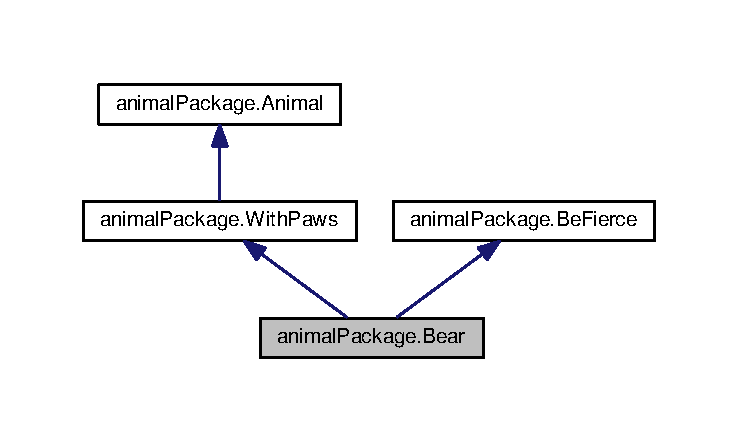
\includegraphics[width=350pt]{classanimal_package_1_1_bear__inherit__graph}
\end{center}
\end{figure}


Collaboration diagram for animal\+Package.\+Bear\+:\nopagebreak
\begin{figure}[H]
\begin{center}
\leavevmode
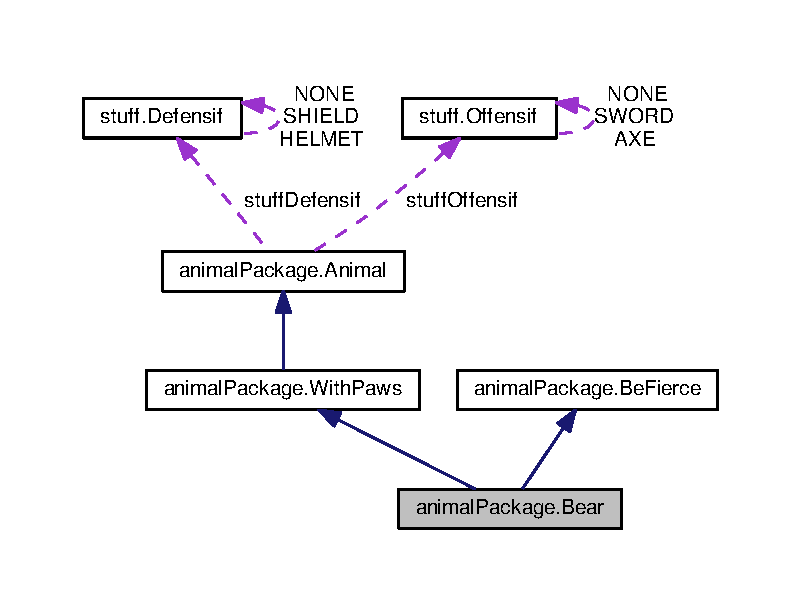
\includegraphics[width=350pt]{classanimal_package_1_1_bear__coll__graph}
\end{center}
\end{figure}
\subsection*{Public Member Functions}
\begin{DoxyCompactItemize}
\item 
\hyperlink{classanimal_package_1_1_bear_a6d8eb57064fac579568c4527acbb8a0f}{Bear} (String new\+Pseudo)
\item 
\hyperlink{classanimal_package_1_1_bear_ab659fd4a52e58d0f5b2018f0829c3d9b}{Bear} (String new\+Pseudo, String new\+Color)
\item 
void \hyperlink{classanimal_package_1_1_bear_a7c978545964edaa05d2e115cc744ad1a}{attack} (\hyperlink{classanimal_package_1_1_animal}{Animal} attacked\+Animal)
\item 
String \hyperlink{classanimal_package_1_1_bear_ae90f660522aeb791abef80920427a0e7}{special\+Action} (\hyperlink{classanimal_package_1_1_animal}{Animal} attacked\+Animal)
\item 
void \hyperlink{classanimal_package_1_1_bear_a8c4bc708619629006e39b5c220e8341b}{scream} ()
\item 
String \hyperlink{classanimal_package_1_1_bear_adb2490fd33a718dc539bd501485a3764}{be\+Fierce} ()
\end{DoxyCompactItemize}
\subsection*{Additional Inherited Members}


\subsection{Detailed Description}
===== Class \hyperlink{classanimal_package_1_1_bear}{Bear} =====

\begin{DoxyAuthor}{Author}
Vincent Reynaert, Nicolas Sobczak 
\end{DoxyAuthor}
\begin{DoxyVersion}{Version}
1.\+03, 11/2016 
\end{DoxyVersion}


\subsection{Constructor \& Destructor Documentation}
\index{animal\+Package\+::\+Bear@{animal\+Package\+::\+Bear}!Bear@{Bear}}
\index{Bear@{Bear}!animal\+Package\+::\+Bear@{animal\+Package\+::\+Bear}}
\subsubsection[{\texorpdfstring{Bear(\+String new\+Pseudo)}{Bear(String newPseudo)}}]{\setlength{\rightskip}{0pt plus 5cm}animal\+Package.\+Bear.\+Bear (
\begin{DoxyParamCaption}
\item[{String}]{new\+Pseudo}
\end{DoxyParamCaption}
)}\hypertarget{classanimal_package_1_1_bear_a6d8eb57064fac579568c4527acbb8a0f}{}\label{classanimal_package_1_1_bear_a6d8eb57064fac579568c4527acbb8a0f}
Constructor


\begin{DoxyParams}{Parameters}
{\em 1} & String = bear\textquotesingle{}s Pseudo \\
\hline
\end{DoxyParams}
\index{animal\+Package\+::\+Bear@{animal\+Package\+::\+Bear}!Bear@{Bear}}
\index{Bear@{Bear}!animal\+Package\+::\+Bear@{animal\+Package\+::\+Bear}}
\subsubsection[{\texorpdfstring{Bear(\+String new\+Pseudo, String new\+Color)}{Bear(String newPseudo, String newColor)}}]{\setlength{\rightskip}{0pt plus 5cm}animal\+Package.\+Bear.\+Bear (
\begin{DoxyParamCaption}
\item[{String}]{new\+Pseudo, }
\item[{String}]{new\+Color}
\end{DoxyParamCaption}
)}\hypertarget{classanimal_package_1_1_bear_ab659fd4a52e58d0f5b2018f0829c3d9b}{}\label{classanimal_package_1_1_bear_ab659fd4a52e58d0f5b2018f0829c3d9b}
Constructor


\begin{DoxyParams}{Parameters}
{\em 1} & String = bear\textquotesingle{}s Pseudo \\
\hline
{\em 1} & String = bear\textquotesingle{}s color \\
\hline
\end{DoxyParams}


\subsection{Member Function Documentation}
\index{animal\+Package\+::\+Bear@{animal\+Package\+::\+Bear}!attack@{attack}}
\index{attack@{attack}!animal\+Package\+::\+Bear@{animal\+Package\+::\+Bear}}
\subsubsection[{\texorpdfstring{attack(\+Animal attacked\+Animal)}{attack(Animal attackedAnimal)}}]{\setlength{\rightskip}{0pt plus 5cm}void animal\+Package.\+Bear.\+attack (
\begin{DoxyParamCaption}
\item[{{\bf Animal}}]{attacked\+Animal}
\end{DoxyParamCaption}
)}\hypertarget{classanimal_package_1_1_bear_a7c978545964edaa05d2e115cc744ad1a}{}\label{classanimal_package_1_1_bear_a7c978545964edaa05d2e115cc744ad1a}
attack \+: function which executes a basic attack


\begin{DoxyParams}{Parameters}
{\em \hyperlink{classanimal_package_1_1_animal}{Animal}} & attacked\+Animal \\
\hline
\end{DoxyParams}
\index{animal\+Package\+::\+Bear@{animal\+Package\+::\+Bear}!be\+Fierce@{be\+Fierce}}
\index{be\+Fierce@{be\+Fierce}!animal\+Package\+::\+Bear@{animal\+Package\+::\+Bear}}
\subsubsection[{\texorpdfstring{be\+Fierce()}{beFierce()}}]{\setlength{\rightskip}{0pt plus 5cm}String animal\+Package.\+Bear.\+be\+Fierce (
\begin{DoxyParamCaption}
{}
\end{DoxyParamCaption}
)}\hypertarget{classanimal_package_1_1_bear_adb2490fd33a718dc539bd501485a3764}{}\label{classanimal_package_1_1_bear_adb2490fd33a718dc539bd501485a3764}
be\+Fierce \+: function which return an adjective to describe behavior

\begin{DoxyReturn}{Returns}
1 String = an adjective 
\end{DoxyReturn}


Implements \hyperlink{interfaceanimal_package_1_1_be_fierce_aaa3925a8d59cbeccc2cb2a6d46d4ba2e}{animal\+Package.\+Be\+Fierce}.

\index{animal\+Package\+::\+Bear@{animal\+Package\+::\+Bear}!scream@{scream}}
\index{scream@{scream}!animal\+Package\+::\+Bear@{animal\+Package\+::\+Bear}}
\subsubsection[{\texorpdfstring{scream()}{scream()}}]{\setlength{\rightskip}{0pt plus 5cm}void animal\+Package.\+Bear.\+scream (
\begin{DoxyParamCaption}
{}
\end{DoxyParamCaption}
)}\hypertarget{classanimal_package_1_1_bear_a8c4bc708619629006e39b5c220e8341b}{}\label{classanimal_package_1_1_bear_a8c4bc708619629006e39b5c220e8341b}
scream \+: function which makes the animal scream \index{animal\+Package\+::\+Bear@{animal\+Package\+::\+Bear}!special\+Action@{special\+Action}}
\index{special\+Action@{special\+Action}!animal\+Package\+::\+Bear@{animal\+Package\+::\+Bear}}
\subsubsection[{\texorpdfstring{special\+Action(\+Animal attacked\+Animal)}{specialAction(Animal attackedAnimal)}}]{\setlength{\rightskip}{0pt plus 5cm}String animal\+Package.\+Bear.\+special\+Action (
\begin{DoxyParamCaption}
\item[{{\bf Animal}}]{attacked\+Animal}
\end{DoxyParamCaption}
)}\hypertarget{classanimal_package_1_1_bear_ae90f660522aeb791abef80920427a0e7}{}\label{classanimal_package_1_1_bear_ae90f660522aeb791abef80920427a0e7}
special\+Action \+: function which executes a special attack For the bear it is damage\+Annulation


\begin{DoxyParams}{Parameters}
{\em \hyperlink{classanimal_package_1_1_animal}{Animal}} & attacked\+Animal \\
\hline
\end{DoxyParams}
\begin{DoxyReturn}{Returns}
String 
\end{DoxyReturn}


The documentation for this class was generated from the following file\+:\begin{DoxyCompactItemize}
\item 
src/animal\+Package/Bear.\+java\end{DoxyCompactItemize}

\hypertarget{interfaceanimal_package_1_1_be_fierce}{}\section{animal\+Package.\+Be\+Fierce Interface Reference}
\label{interfaceanimal_package_1_1_be_fierce}\index{animal\+Package.\+Be\+Fierce@{animal\+Package.\+Be\+Fierce}}


Inheritance diagram for animal\+Package.\+Be\+Fierce\+:\nopagebreak
\begin{figure}[H]
\begin{center}
\leavevmode
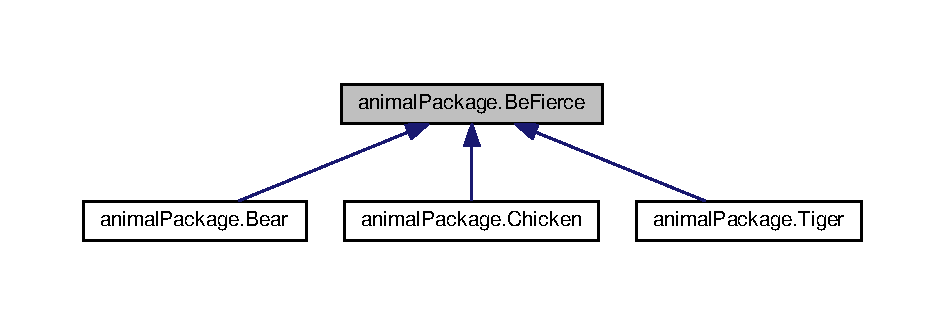
\includegraphics[width=350pt]{interfaceanimal_package_1_1_be_fierce__inherit__graph}
\end{center}
\end{figure}
\subsection*{Public Member Functions}
\begin{DoxyCompactItemize}
\item 
String \hyperlink{interfaceanimal_package_1_1_be_fierce_aaa3925a8d59cbeccc2cb2a6d46d4ba2e}{be\+Fierce} ()
\end{DoxyCompactItemize}


\subsection{Detailed Description}
===== interface \hyperlink{interfaceanimal_package_1_1_be_fierce}{Be\+Fierce} =====

\begin{DoxyAuthor}{Author}
Vincent Reynaert, Nicolas Sobczak 
\end{DoxyAuthor}
\begin{DoxyVersion}{Version}
1.\+01, 11/2016 
\end{DoxyVersion}


\subsection{Member Function Documentation}
\index{animal\+Package\+::\+Be\+Fierce@{animal\+Package\+::\+Be\+Fierce}!be\+Fierce@{be\+Fierce}}
\index{be\+Fierce@{be\+Fierce}!animal\+Package\+::\+Be\+Fierce@{animal\+Package\+::\+Be\+Fierce}}
\subsubsection[{\texorpdfstring{be\+Fierce()}{beFierce()}}]{\setlength{\rightskip}{0pt plus 5cm}String animal\+Package.\+Be\+Fierce.\+be\+Fierce (
\begin{DoxyParamCaption}
{}
\end{DoxyParamCaption}
)}\hypertarget{interfaceanimal_package_1_1_be_fierce_aaa3925a8d59cbeccc2cb2a6d46d4ba2e}{}\label{interfaceanimal_package_1_1_be_fierce_aaa3925a8d59cbeccc2cb2a6d46d4ba2e}
be\+Fierce \+: function which return an adjective to describe behavior

\begin{DoxyReturn}{Returns}
1 String = an adjective 
\end{DoxyReturn}


Implemented in \hyperlink{classanimal_package_1_1_bear_adb2490fd33a718dc539bd501485a3764}{animal\+Package.\+Bear}, \hyperlink{classanimal_package_1_1_chicken_acbab445b817267020bad14971bc7aade}{animal\+Package.\+Chicken}, and \hyperlink{classanimal_package_1_1_tiger_a9c941af145fed9f1d71176ff6a752e16}{animal\+Package.\+Tiger}.



The documentation for this interface was generated from the following file\+:\begin{DoxyCompactItemize}
\item 
src/animal\+Package/Be\+Fierce.\+java\end{DoxyCompactItemize}

\hypertarget{classanimal_package_1_1_chicken}{}\section{animal\+Package.\+Chicken Class Reference}
\label{classanimal_package_1_1_chicken}\index{animal\+Package.\+Chicken@{animal\+Package.\+Chicken}}


Inheritance diagram for animal\+Package.\+Chicken\+:\nopagebreak
\begin{figure}[H]
\begin{center}
\leavevmode
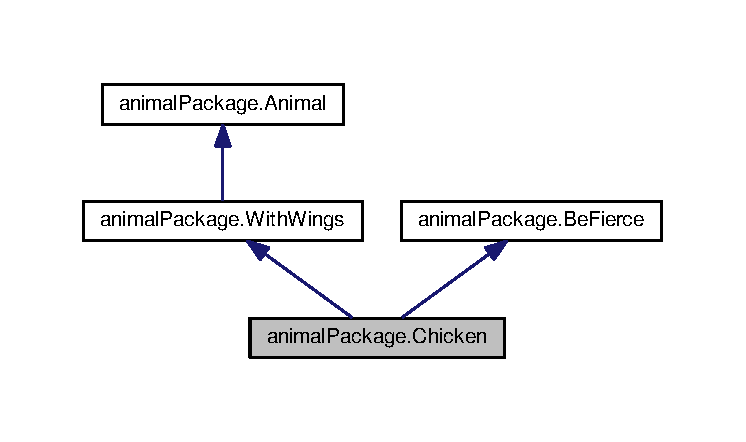
\includegraphics[width=350pt]{classanimal_package_1_1_chicken__inherit__graph}
\end{center}
\end{figure}


Collaboration diagram for animal\+Package.\+Chicken\+:\nopagebreak
\begin{figure}[H]
\begin{center}
\leavevmode
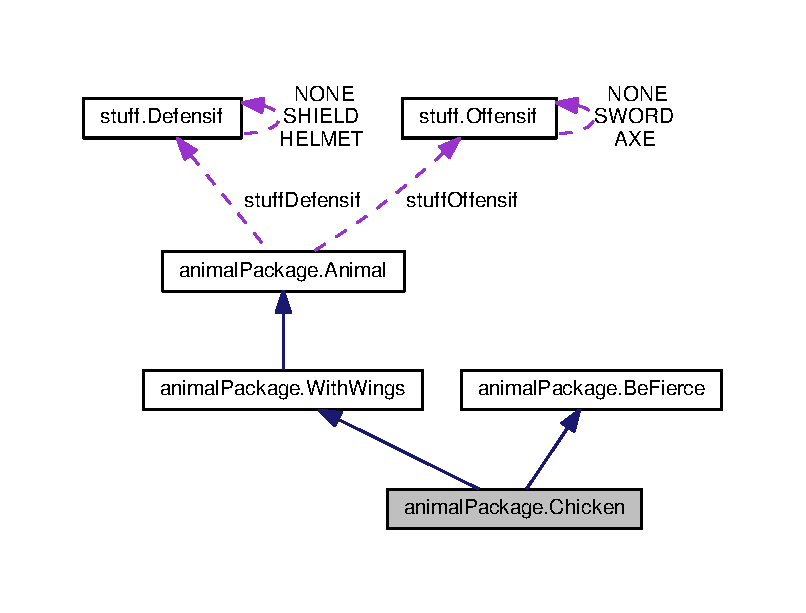
\includegraphics[width=350pt]{classanimal_package_1_1_chicken__coll__graph}
\end{center}
\end{figure}
\subsection*{Public Member Functions}
\begin{DoxyCompactItemize}
\item 
\hyperlink{classanimal_package_1_1_chicken_a40c2ff20215142df5863c92b5cda668f}{Chicken} (String new\+Pseudo)
\item 
\hyperlink{classanimal_package_1_1_chicken_ac9d80790ffc67776ea2bf41dd0d1cb8c}{Chicken} (String new\+Pseudo, String new\+Color)
\item 
void \hyperlink{classanimal_package_1_1_chicken_af7083b18b61b5706ac907af79e46990a}{attack} (\hyperlink{classanimal_package_1_1_animal}{Animal} attacked\+Animal)
\item 
String \hyperlink{classanimal_package_1_1_chicken_a14b6e124c1b2655faabf125719113ad1}{special\+Action} (\hyperlink{classanimal_package_1_1_animal}{Animal} attacked\+Animal)
\item 
void \hyperlink{classanimal_package_1_1_chicken_a14f06d93a9c7b0dc32d68bc29d6dd69c}{scream} ()
\item 
String \hyperlink{classanimal_package_1_1_chicken_acbab445b817267020bad14971bc7aade}{be\+Fierce} ()
\end{DoxyCompactItemize}
\subsection*{Additional Inherited Members}


\subsection{Detailed Description}
===== Class \hyperlink{classanimal_package_1_1_chicken}{Chicken} =====

\begin{DoxyAuthor}{Author}
Vincent Reynaert, Nicolas Sobczak 
\end{DoxyAuthor}
\begin{DoxyVersion}{Version}
1.\+03, 11/2016 
\end{DoxyVersion}


\subsection{Constructor \& Destructor Documentation}
\index{animal\+Package\+::\+Chicken@{animal\+Package\+::\+Chicken}!Chicken@{Chicken}}
\index{Chicken@{Chicken}!animal\+Package\+::\+Chicken@{animal\+Package\+::\+Chicken}}
\subsubsection[{\texorpdfstring{Chicken(\+String new\+Pseudo)}{Chicken(String newPseudo)}}]{\setlength{\rightskip}{0pt plus 5cm}animal\+Package.\+Chicken.\+Chicken (
\begin{DoxyParamCaption}
\item[{String}]{new\+Pseudo}
\end{DoxyParamCaption}
)}\hypertarget{classanimal_package_1_1_chicken_a40c2ff20215142df5863c92b5cda668f}{}\label{classanimal_package_1_1_chicken_a40c2ff20215142df5863c92b5cda668f}
Constructor


\begin{DoxyParams}{Parameters}
{\em 1} & String = chicken\textquotesingle{}s Pseudo \\
\hline
\end{DoxyParams}
\index{animal\+Package\+::\+Chicken@{animal\+Package\+::\+Chicken}!Chicken@{Chicken}}
\index{Chicken@{Chicken}!animal\+Package\+::\+Chicken@{animal\+Package\+::\+Chicken}}
\subsubsection[{\texorpdfstring{Chicken(\+String new\+Pseudo, String new\+Color)}{Chicken(String newPseudo, String newColor)}}]{\setlength{\rightskip}{0pt plus 5cm}animal\+Package.\+Chicken.\+Chicken (
\begin{DoxyParamCaption}
\item[{String}]{new\+Pseudo, }
\item[{String}]{new\+Color}
\end{DoxyParamCaption}
)}\hypertarget{classanimal_package_1_1_chicken_ac9d80790ffc67776ea2bf41dd0d1cb8c}{}\label{classanimal_package_1_1_chicken_ac9d80790ffc67776ea2bf41dd0d1cb8c}
Constructor


\begin{DoxyParams}{Parameters}
{\em 1} & String = chicken\textquotesingle{}s Pseudo \\
\hline
{\em 1} & String = chicken\textquotesingle{}s color \\
\hline
\end{DoxyParams}


\subsection{Member Function Documentation}
\index{animal\+Package\+::\+Chicken@{animal\+Package\+::\+Chicken}!attack@{attack}}
\index{attack@{attack}!animal\+Package\+::\+Chicken@{animal\+Package\+::\+Chicken}}
\subsubsection[{\texorpdfstring{attack(\+Animal attacked\+Animal)}{attack(Animal attackedAnimal)}}]{\setlength{\rightskip}{0pt plus 5cm}void animal\+Package.\+Chicken.\+attack (
\begin{DoxyParamCaption}
\item[{{\bf Animal}}]{attacked\+Animal}
\end{DoxyParamCaption}
)}\hypertarget{classanimal_package_1_1_chicken_af7083b18b61b5706ac907af79e46990a}{}\label{classanimal_package_1_1_chicken_af7083b18b61b5706ac907af79e46990a}
attack \+: function which executes a basic attack


\begin{DoxyParams}{Parameters}
{\em \hyperlink{classanimal_package_1_1_animal}{Animal}} & attacked\+Animal \\
\hline
\end{DoxyParams}
\begin{DoxyReturn}{Returns}
String 
\end{DoxyReturn}
\index{animal\+Package\+::\+Chicken@{animal\+Package\+::\+Chicken}!be\+Fierce@{be\+Fierce}}
\index{be\+Fierce@{be\+Fierce}!animal\+Package\+::\+Chicken@{animal\+Package\+::\+Chicken}}
\subsubsection[{\texorpdfstring{be\+Fierce()}{beFierce()}}]{\setlength{\rightskip}{0pt plus 5cm}String animal\+Package.\+Chicken.\+be\+Fierce (
\begin{DoxyParamCaption}
{}
\end{DoxyParamCaption}
)}\hypertarget{classanimal_package_1_1_chicken_acbab445b817267020bad14971bc7aade}{}\label{classanimal_package_1_1_chicken_acbab445b817267020bad14971bc7aade}
be\+Fierce \+: function which return an adjective to describe behavior

\begin{DoxyReturn}{Returns}
1 String = an adjective 
\end{DoxyReturn}


Implements \hyperlink{interfaceanimal_package_1_1_be_fierce_aaa3925a8d59cbeccc2cb2a6d46d4ba2e}{animal\+Package.\+Be\+Fierce}.

\index{animal\+Package\+::\+Chicken@{animal\+Package\+::\+Chicken}!scream@{scream}}
\index{scream@{scream}!animal\+Package\+::\+Chicken@{animal\+Package\+::\+Chicken}}
\subsubsection[{\texorpdfstring{scream()}{scream()}}]{\setlength{\rightskip}{0pt plus 5cm}void animal\+Package.\+Chicken.\+scream (
\begin{DoxyParamCaption}
{}
\end{DoxyParamCaption}
)}\hypertarget{classanimal_package_1_1_chicken_a14f06d93a9c7b0dc32d68bc29d6dd69c}{}\label{classanimal_package_1_1_chicken_a14f06d93a9c7b0dc32d68bc29d6dd69c}
scream \+: function which makes the animal scream \index{animal\+Package\+::\+Chicken@{animal\+Package\+::\+Chicken}!special\+Action@{special\+Action}}
\index{special\+Action@{special\+Action}!animal\+Package\+::\+Chicken@{animal\+Package\+::\+Chicken}}
\subsubsection[{\texorpdfstring{special\+Action(\+Animal attacked\+Animal)}{specialAction(Animal attackedAnimal)}}]{\setlength{\rightskip}{0pt plus 5cm}String animal\+Package.\+Chicken.\+special\+Action (
\begin{DoxyParamCaption}
\item[{{\bf Animal}}]{attacked\+Animal}
\end{DoxyParamCaption}
)}\hypertarget{classanimal_package_1_1_chicken_a14b6e124c1b2655faabf125719113ad1}{}\label{classanimal_package_1_1_chicken_a14b6e124c1b2655faabf125719113ad1}
special\+Action \+: function which executes a special attack


\begin{DoxyParams}{Parameters}
{\em \hyperlink{classanimal_package_1_1_animal}{Animal}} & attacked\+Animal \\
\hline
\end{DoxyParams}


The documentation for this class was generated from the following file\+:\begin{DoxyCompactItemize}
\item 
src/animal\+Package/Chicken.\+java\end{DoxyCompactItemize}

\hypertarget{classcube_environment_1_1_cube_environment}{}\section{cube\+Environment.\+Cube\+Environment Class Reference}
\label{classcube_environment_1_1_cube_environment}\index{cube\+Environment.\+Cube\+Environment@{cube\+Environment.\+Cube\+Environment}}
\subsection*{Public Member Functions}
\begin{DoxyCompactItemize}
\item 
\hyperlink{classcube_environment_1_1_cube_environment_a7aab28baa3136e834671a2b39031a15c}{Cube\+Environment} ()
\item 
\hyperlink{classcube_environment_1_1_cube_environment_a499bd8a94afd3a4038e5d97f73eb1044}{Cube\+Environment} (\hyperlink{classplayer_package_1_1_player}{Player} playerI)
\item 
\hyperlink{classspace_objects_1_1_spacecraft}{Spacecraft} \hyperlink{classcube_environment_1_1_cube_environment_a6d0eb90b0c6cf053139c4ac4ff76e9f0}{get\+Spacecraft} ()
\item 
\hyperlink{classspace_objects_1_1_meteorite}{Meteorite} \hyperlink{classcube_environment_1_1_cube_environment_aeda6bdc32698e0eac05a5dc860a3d944}{get\+Meteorite\+Small} ()
\item 
\hyperlink{classspace_objects_1_1_meteorite}{Meteorite} \hyperlink{classcube_environment_1_1_cube_environment_a7a1a3509cd7fbc80c2dcfad45fa04087}{get\+Meteorite\+Medium} ()
\item 
\hyperlink{classspace_objects_1_1_meteorite}{Meteorite} \hyperlink{classcube_environment_1_1_cube_environment_a2e84a4caf92462f912c3340c162014c6}{get\+Meteorite\+Big} ()
\item 
void \hyperlink{classcube_environment_1_1_cube_environment_a4efde03b2357b31b564ece4c3f66f6d5}{set\+Spacecraft} (\hyperlink{classspace_objects_1_1_spacecraft}{Spacecraft} new\+Spacecraft)
\item 
void \hyperlink{classcube_environment_1_1_cube_environment_ab263bc0754be2dcac50300a753cf0a38}{set\+Meteorite\+Small} (\hyperlink{classspace_objects_1_1_meteorite}{Meteorite} new\+Meteorite)
\item 
void \hyperlink{classcube_environment_1_1_cube_environment_ae6cba09c65695965b9a08eb7e38de758}{set\+Meteorite\+Medium} (\hyperlink{classspace_objects_1_1_meteorite}{Meteorite} new\+Meteorite)
\item 
void \hyperlink{classcube_environment_1_1_cube_environment_af4014fd21f085dd8c2514b56d97f9d4d}{set\+Meteorite\+Big} (\hyperlink{classspace_objects_1_1_meteorite}{Meteorite} new\+Meteorite)
\item 
\hyperlink{enumspace_objects_1_1_positions_cube}{Positions\+Cube} {\bfseries int\+To\+Position} (int position)  throws Position\+Exception \hypertarget{classcube_environment_1_1_cube_environment_ac7f7a9248c1008fcb49e75a173aa9fee}{}\label{classcube_environment_1_1_cube_environment_ac7f7a9248c1008fcb49e75a173aa9fee}

\item 
void {\bfseries relocate\+All\+Ufo} ()\hypertarget{classcube_environment_1_1_cube_environment_ab04dc4b7da575cbb5efbc2c92aacedce}{}\label{classcube_environment_1_1_cube_environment_ab04dc4b7da575cbb5efbc2c92aacedce}

\end{DoxyCompactItemize}


\subsection{Detailed Description}
===== Class \hyperlink{classcube_environment_1_1_cube_environment}{Cube\+Environment} =====

\begin{DoxyAuthor}{Author}
Vincent Reynaert, Nicolas Sobczak 
\end{DoxyAuthor}
\begin{DoxyVersion}{Version}
1.\+03, 11/2016 
\end{DoxyVersion}


\subsection{Constructor \& Destructor Documentation}
\index{cube\+Environment\+::\+Cube\+Environment@{cube\+Environment\+::\+Cube\+Environment}!Cube\+Environment@{Cube\+Environment}}
\index{Cube\+Environment@{Cube\+Environment}!cube\+Environment\+::\+Cube\+Environment@{cube\+Environment\+::\+Cube\+Environment}}
\subsubsection[{\texorpdfstring{Cube\+Environment()}{CubeEnvironment()}}]{\setlength{\rightskip}{0pt plus 5cm}cube\+Environment.\+Cube\+Environment.\+Cube\+Environment (
\begin{DoxyParamCaption}
{}
\end{DoxyParamCaption}
)}\hypertarget{classcube_environment_1_1_cube_environment_a7aab28baa3136e834671a2b39031a15c}{}\label{classcube_environment_1_1_cube_environment_a7aab28baa3136e834671a2b39031a15c}
Constructor \index{cube\+Environment\+::\+Cube\+Environment@{cube\+Environment\+::\+Cube\+Environment}!Cube\+Environment@{Cube\+Environment}}
\index{Cube\+Environment@{Cube\+Environment}!cube\+Environment\+::\+Cube\+Environment@{cube\+Environment\+::\+Cube\+Environment}}
\subsubsection[{\texorpdfstring{Cube\+Environment(\+Player player\+I)}{CubeEnvironment(Player playerI)}}]{\setlength{\rightskip}{0pt plus 5cm}cube\+Environment.\+Cube\+Environment.\+Cube\+Environment (
\begin{DoxyParamCaption}
\item[{{\bf Player}}]{playerI}
\end{DoxyParamCaption}
)}\hypertarget{classcube_environment_1_1_cube_environment_a499bd8a94afd3a4038e5d97f73eb1044}{}\label{classcube_environment_1_1_cube_environment_a499bd8a94afd3a4038e5d97f73eb1044}
Constuctor


\begin{DoxyParams}{Parameters}
{\em 1} & Player = playerI \\
\hline
\end{DoxyParams}


\subsection{Member Function Documentation}
\index{cube\+Environment\+::\+Cube\+Environment@{cube\+Environment\+::\+Cube\+Environment}!get\+Meteorite\+Big@{get\+Meteorite\+Big}}
\index{get\+Meteorite\+Big@{get\+Meteorite\+Big}!cube\+Environment\+::\+Cube\+Environment@{cube\+Environment\+::\+Cube\+Environment}}
\subsubsection[{\texorpdfstring{get\+Meteorite\+Big()}{getMeteoriteBig()}}]{\setlength{\rightskip}{0pt plus 5cm}{\bf Meteorite} cube\+Environment.\+Cube\+Environment.\+get\+Meteorite\+Big (
\begin{DoxyParamCaption}
{}
\end{DoxyParamCaption}
)}\hypertarget{classcube_environment_1_1_cube_environment_a2e84a4caf92462f912c3340c162014c6}{}\label{classcube_environment_1_1_cube_environment_a2e84a4caf92462f912c3340c162014c6}
Get \hyperlink{classcube_environment_1_1_cube_environment}{Cube\+Environment} meteorite\+Big

\begin{DoxyReturn}{Returns}
1 Meteorite = meteorite\+Big 
\end{DoxyReturn}
\index{cube\+Environment\+::\+Cube\+Environment@{cube\+Environment\+::\+Cube\+Environment}!get\+Meteorite\+Medium@{get\+Meteorite\+Medium}}
\index{get\+Meteorite\+Medium@{get\+Meteorite\+Medium}!cube\+Environment\+::\+Cube\+Environment@{cube\+Environment\+::\+Cube\+Environment}}
\subsubsection[{\texorpdfstring{get\+Meteorite\+Medium()}{getMeteoriteMedium()}}]{\setlength{\rightskip}{0pt plus 5cm}{\bf Meteorite} cube\+Environment.\+Cube\+Environment.\+get\+Meteorite\+Medium (
\begin{DoxyParamCaption}
{}
\end{DoxyParamCaption}
)}\hypertarget{classcube_environment_1_1_cube_environment_a7a1a3509cd7fbc80c2dcfad45fa04087}{}\label{classcube_environment_1_1_cube_environment_a7a1a3509cd7fbc80c2dcfad45fa04087}
Get \hyperlink{classcube_environment_1_1_cube_environment}{Cube\+Environment} meteorite\+Medium

\begin{DoxyReturn}{Returns}
1 Meteorite = meteorite\+Medium 
\end{DoxyReturn}
\index{cube\+Environment\+::\+Cube\+Environment@{cube\+Environment\+::\+Cube\+Environment}!get\+Meteorite\+Small@{get\+Meteorite\+Small}}
\index{get\+Meteorite\+Small@{get\+Meteorite\+Small}!cube\+Environment\+::\+Cube\+Environment@{cube\+Environment\+::\+Cube\+Environment}}
\subsubsection[{\texorpdfstring{get\+Meteorite\+Small()}{getMeteoriteSmall()}}]{\setlength{\rightskip}{0pt plus 5cm}{\bf Meteorite} cube\+Environment.\+Cube\+Environment.\+get\+Meteorite\+Small (
\begin{DoxyParamCaption}
{}
\end{DoxyParamCaption}
)}\hypertarget{classcube_environment_1_1_cube_environment_aeda6bdc32698e0eac05a5dc860a3d944}{}\label{classcube_environment_1_1_cube_environment_aeda6bdc32698e0eac05a5dc860a3d944}
Get \hyperlink{classcube_environment_1_1_cube_environment}{Cube\+Environment} meteorite\+Small

\begin{DoxyReturn}{Returns}
1 Meteorite = meteorite\+Small 
\end{DoxyReturn}
\index{cube\+Environment\+::\+Cube\+Environment@{cube\+Environment\+::\+Cube\+Environment}!get\+Spacecraft@{get\+Spacecraft}}
\index{get\+Spacecraft@{get\+Spacecraft}!cube\+Environment\+::\+Cube\+Environment@{cube\+Environment\+::\+Cube\+Environment}}
\subsubsection[{\texorpdfstring{get\+Spacecraft()}{getSpacecraft()}}]{\setlength{\rightskip}{0pt plus 5cm}{\bf Spacecraft} cube\+Environment.\+Cube\+Environment.\+get\+Spacecraft (
\begin{DoxyParamCaption}
{}
\end{DoxyParamCaption}
)}\hypertarget{classcube_environment_1_1_cube_environment_a6d0eb90b0c6cf053139c4ac4ff76e9f0}{}\label{classcube_environment_1_1_cube_environment_a6d0eb90b0c6cf053139c4ac4ff76e9f0}
Get \hyperlink{classcube_environment_1_1_cube_environment}{Cube\+Environment} spacecraft

\begin{DoxyReturn}{Returns}
1 Spacecraft = spacecraft 
\end{DoxyReturn}
\index{cube\+Environment\+::\+Cube\+Environment@{cube\+Environment\+::\+Cube\+Environment}!set\+Meteorite\+Big@{set\+Meteorite\+Big}}
\index{set\+Meteorite\+Big@{set\+Meteorite\+Big}!cube\+Environment\+::\+Cube\+Environment@{cube\+Environment\+::\+Cube\+Environment}}
\subsubsection[{\texorpdfstring{set\+Meteorite\+Big(\+Meteorite new\+Meteorite)}{setMeteoriteBig(Meteorite newMeteorite)}}]{\setlength{\rightskip}{0pt plus 5cm}void cube\+Environment.\+Cube\+Environment.\+set\+Meteorite\+Big (
\begin{DoxyParamCaption}
\item[{{\bf Meteorite}}]{new\+Meteorite}
\end{DoxyParamCaption}
)}\hypertarget{classcube_environment_1_1_cube_environment_af4014fd21f085dd8c2514b56d97f9d4d}{}\label{classcube_environment_1_1_cube_environment_af4014fd21f085dd8c2514b56d97f9d4d}
Set \hyperlink{classcube_environment_1_1_cube_environment}{Cube\+Environment} meteorite\+Big


\begin{DoxyParams}{Parameters}
{\em 1} & Meteorite = new\+Meteorite \\
\hline
\end{DoxyParams}
\index{cube\+Environment\+::\+Cube\+Environment@{cube\+Environment\+::\+Cube\+Environment}!set\+Meteorite\+Medium@{set\+Meteorite\+Medium}}
\index{set\+Meteorite\+Medium@{set\+Meteorite\+Medium}!cube\+Environment\+::\+Cube\+Environment@{cube\+Environment\+::\+Cube\+Environment}}
\subsubsection[{\texorpdfstring{set\+Meteorite\+Medium(\+Meteorite new\+Meteorite)}{setMeteoriteMedium(Meteorite newMeteorite)}}]{\setlength{\rightskip}{0pt plus 5cm}void cube\+Environment.\+Cube\+Environment.\+set\+Meteorite\+Medium (
\begin{DoxyParamCaption}
\item[{{\bf Meteorite}}]{new\+Meteorite}
\end{DoxyParamCaption}
)}\hypertarget{classcube_environment_1_1_cube_environment_ae6cba09c65695965b9a08eb7e38de758}{}\label{classcube_environment_1_1_cube_environment_ae6cba09c65695965b9a08eb7e38de758}
Set \hyperlink{classcube_environment_1_1_cube_environment}{Cube\+Environment} meteorite\+Medium


\begin{DoxyParams}{Parameters}
{\em 1} & Meteorite = new\+Meteorite \\
\hline
\end{DoxyParams}
\index{cube\+Environment\+::\+Cube\+Environment@{cube\+Environment\+::\+Cube\+Environment}!set\+Meteorite\+Small@{set\+Meteorite\+Small}}
\index{set\+Meteorite\+Small@{set\+Meteorite\+Small}!cube\+Environment\+::\+Cube\+Environment@{cube\+Environment\+::\+Cube\+Environment}}
\subsubsection[{\texorpdfstring{set\+Meteorite\+Small(\+Meteorite new\+Meteorite)}{setMeteoriteSmall(Meteorite newMeteorite)}}]{\setlength{\rightskip}{0pt plus 5cm}void cube\+Environment.\+Cube\+Environment.\+set\+Meteorite\+Small (
\begin{DoxyParamCaption}
\item[{{\bf Meteorite}}]{new\+Meteorite}
\end{DoxyParamCaption}
)}\hypertarget{classcube_environment_1_1_cube_environment_ab263bc0754be2dcac50300a753cf0a38}{}\label{classcube_environment_1_1_cube_environment_ab263bc0754be2dcac50300a753cf0a38}
Set \hyperlink{classcube_environment_1_1_cube_environment}{Cube\+Environment} meteorite\+Small


\begin{DoxyParams}{Parameters}
{\em 1} & Meteorite = new\+Meteorite \\
\hline
\end{DoxyParams}
\index{cube\+Environment\+::\+Cube\+Environment@{cube\+Environment\+::\+Cube\+Environment}!set\+Spacecraft@{set\+Spacecraft}}
\index{set\+Spacecraft@{set\+Spacecraft}!cube\+Environment\+::\+Cube\+Environment@{cube\+Environment\+::\+Cube\+Environment}}
\subsubsection[{\texorpdfstring{set\+Spacecraft(\+Spacecraft new\+Spacecraft)}{setSpacecraft(Spacecraft newSpacecraft)}}]{\setlength{\rightskip}{0pt plus 5cm}void cube\+Environment.\+Cube\+Environment.\+set\+Spacecraft (
\begin{DoxyParamCaption}
\item[{{\bf Spacecraft}}]{new\+Spacecraft}
\end{DoxyParamCaption}
)}\hypertarget{classcube_environment_1_1_cube_environment_a4efde03b2357b31b564ece4c3f66f6d5}{}\label{classcube_environment_1_1_cube_environment_a4efde03b2357b31b564ece4c3f66f6d5}
Set \hyperlink{classcube_environment_1_1_cube_environment}{Cube\+Environment} spacecraft


\begin{DoxyParams}{Parameters}
{\em 1} & Spacecraft = new\+Spacecraft \\
\hline
\end{DoxyParams}


The documentation for this class was generated from the following file\+:\begin{DoxyCompactItemize}
\item 
src/cube\+Environment/Cube\+Environment.\+java\end{DoxyCompactItemize}

\hypertarget{classstuff_1_1_defensif}{}\section{stuff.\+Defensif Class Reference}
\label{classstuff_1_1_defensif}\index{stuff.\+Defensif@{stuff.\+Defensif}}


Collaboration diagram for stuff.\+Defensif\+:\nopagebreak
\begin{figure}[H]
\begin{center}
\leavevmode
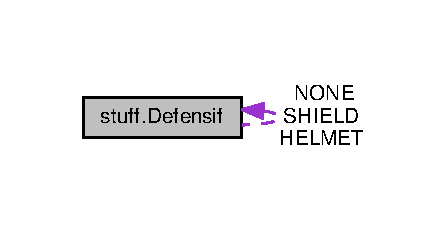
\includegraphics[width=215pt]{classstuff_1_1_defensif__coll__graph}
\end{center}
\end{figure}
\subsection*{Public Member Functions}
\begin{DoxyCompactItemize}
\item 
\hyperlink{classstuff_1_1_defensif_a80561aaf769f44326898b42fb6858bef}{Defensif} (Integer new\+Bonus\+Value)
\item 
void \hyperlink{classstuff_1_1_defensif_a321e58e3129d7e11e4f67b5217713cc8}{set\+Bonus\+Resistance} (Integer new\+Bonus\+Value)
\item 
Integer \hyperlink{classstuff_1_1_defensif_ac92baf4d044b06d44086c54e6099cad2}{get\+Bonus\+Resistance} ()
\end{DoxyCompactItemize}
\subsection*{Static Public Attributes}
\begin{DoxyCompactItemize}
\item 
static final \hyperlink{classstuff_1_1_defensif}{Defensif} \hyperlink{classstuff_1_1_defensif_adf59790d842ebf28a331743caebc2790}{H\+E\+L\+M\+ET} = new \hyperlink{classstuff_1_1_defensif}{Defensif}(5)
\item 
static final \hyperlink{classstuff_1_1_defensif}{Defensif} \hyperlink{classstuff_1_1_defensif_abb7ed080847ab7471ae33d9eecb2a80f}{S\+H\+I\+E\+LD} = new \hyperlink{classstuff_1_1_defensif}{Defensif}(10)
\item 
static final \hyperlink{classstuff_1_1_defensif}{Defensif} \hyperlink{classstuff_1_1_defensif_ad74fec67a8e1ecf651de6078ebb89f8a}{N\+O\+NE} = new \hyperlink{classstuff_1_1_defensif}{Defensif}(0)
\end{DoxyCompactItemize}


\subsection{Detailed Description}
===== Class \hyperlink{classstuff_1_1_defensif}{Defensif} =====

\begin{DoxyAuthor}{Author}
Vincent Reynaert, Nicolas Sobczak 
\end{DoxyAuthor}
\begin{DoxyVersion}{Version}
1.\+02, 11/2016 
\end{DoxyVersion}


\subsection{Constructor \& Destructor Documentation}
\index{stuff\+::\+Defensif@{stuff\+::\+Defensif}!Defensif@{Defensif}}
\index{Defensif@{Defensif}!stuff\+::\+Defensif@{stuff\+::\+Defensif}}
\subsubsection[{\texorpdfstring{Defensif(\+Integer new\+Bonus\+Value)}{Defensif(Integer newBonusValue)}}]{\setlength{\rightskip}{0pt plus 5cm}stuff.\+Defensif.\+Defensif (
\begin{DoxyParamCaption}
\item[{Integer}]{new\+Bonus\+Value}
\end{DoxyParamCaption}
)}\hypertarget{classstuff_1_1_defensif_a80561aaf769f44326898b42fb6858bef}{}\label{classstuff_1_1_defensif_a80561aaf769f44326898b42fb6858bef}
Constructor


\begin{DoxyParams}{Parameters}
{\em int} & new\+Bonus\+Value \\
\hline
\end{DoxyParams}


\subsection{Member Function Documentation}
\index{stuff\+::\+Defensif@{stuff\+::\+Defensif}!get\+Bonus\+Resistance@{get\+Bonus\+Resistance}}
\index{get\+Bonus\+Resistance@{get\+Bonus\+Resistance}!stuff\+::\+Defensif@{stuff\+::\+Defensif}}
\subsubsection[{\texorpdfstring{get\+Bonus\+Resistance()}{getBonusResistance()}}]{\setlength{\rightskip}{0pt plus 5cm}Integer stuff.\+Defensif.\+get\+Bonus\+Resistance (
\begin{DoxyParamCaption}
{}
\end{DoxyParamCaption}
)}\hypertarget{classstuff_1_1_defensif_ac92baf4d044b06d44086c54e6099cad2}{}\label{classstuff_1_1_defensif_ac92baf4d044b06d44086c54e6099cad2}
Get the bonus\+Resistance value

\begin{DoxyReturn}{Returns}
int bonus\+Resistance 
\end{DoxyReturn}
\index{stuff\+::\+Defensif@{stuff\+::\+Defensif}!set\+Bonus\+Resistance@{set\+Bonus\+Resistance}}
\index{set\+Bonus\+Resistance@{set\+Bonus\+Resistance}!stuff\+::\+Defensif@{stuff\+::\+Defensif}}
\subsubsection[{\texorpdfstring{set\+Bonus\+Resistance(\+Integer new\+Bonus\+Value)}{setBonusResistance(Integer newBonusValue)}}]{\setlength{\rightskip}{0pt plus 5cm}void stuff.\+Defensif.\+set\+Bonus\+Resistance (
\begin{DoxyParamCaption}
\item[{Integer}]{new\+Bonus\+Value}
\end{DoxyParamCaption}
)}\hypertarget{classstuff_1_1_defensif_a321e58e3129d7e11e4f67b5217713cc8}{}\label{classstuff_1_1_defensif_a321e58e3129d7e11e4f67b5217713cc8}
Set the bonus\+Resistance


\begin{DoxyParams}{Parameters}
{\em int} & new\+Bonus\+Value \\
\hline
\end{DoxyParams}


\subsection{Member Data Documentation}
\index{stuff\+::\+Defensif@{stuff\+::\+Defensif}!H\+E\+L\+M\+ET@{H\+E\+L\+M\+ET}}
\index{H\+E\+L\+M\+ET@{H\+E\+L\+M\+ET}!stuff\+::\+Defensif@{stuff\+::\+Defensif}}
\subsubsection[{\texorpdfstring{H\+E\+L\+M\+ET}{HELMET}}]{\setlength{\rightskip}{0pt plus 5cm}final {\bf Defensif} stuff.\+Defensif.\+H\+E\+L\+M\+ET = new {\bf Defensif}(5)\hspace{0.3cm}{\ttfamily [static]}}\hypertarget{classstuff_1_1_defensif_adf59790d842ebf28a331743caebc2790}{}\label{classstuff_1_1_defensif_adf59790d842ebf28a331743caebc2790}
Increases the resistance of 5 \index{stuff\+::\+Defensif@{stuff\+::\+Defensif}!N\+O\+NE@{N\+O\+NE}}
\index{N\+O\+NE@{N\+O\+NE}!stuff\+::\+Defensif@{stuff\+::\+Defensif}}
\subsubsection[{\texorpdfstring{N\+O\+NE}{NONE}}]{\setlength{\rightskip}{0pt plus 5cm}final {\bf Defensif} stuff.\+Defensif.\+N\+O\+NE = new {\bf Defensif}(0)\hspace{0.3cm}{\ttfamily [static]}}\hypertarget{classstuff_1_1_defensif_ad74fec67a8e1ecf651de6078ebb89f8a}{}\label{classstuff_1_1_defensif_ad74fec67a8e1ecf651de6078ebb89f8a}
Doesn\textquotesingle{}t increase the resistance \index{stuff\+::\+Defensif@{stuff\+::\+Defensif}!S\+H\+I\+E\+LD@{S\+H\+I\+E\+LD}}
\index{S\+H\+I\+E\+LD@{S\+H\+I\+E\+LD}!stuff\+::\+Defensif@{stuff\+::\+Defensif}}
\subsubsection[{\texorpdfstring{S\+H\+I\+E\+LD}{SHIELD}}]{\setlength{\rightskip}{0pt plus 5cm}final {\bf Defensif} stuff.\+Defensif.\+S\+H\+I\+E\+LD = new {\bf Defensif}(10)\hspace{0.3cm}{\ttfamily [static]}}\hypertarget{classstuff_1_1_defensif_abb7ed080847ab7471ae33d9eecb2a80f}{}\label{classstuff_1_1_defensif_abb7ed080847ab7471ae33d9eecb2a80f}
Increases the resistance of 10 

The documentation for this class was generated from the following file\+:\begin{DoxyCompactItemize}
\item 
src/stuff/Defensif.\+java\end{DoxyCompactItemize}

\hypertarget{classanimal_package_1_1_duck}{}\section{animal\+Package.\+Duck Class Reference}
\label{classanimal_package_1_1_duck}\index{animal\+Package.\+Duck@{animal\+Package.\+Duck}}


Inheritance diagram for animal\+Package.\+Duck\+:\nopagebreak
\begin{figure}[H]
\begin{center}
\leavevmode
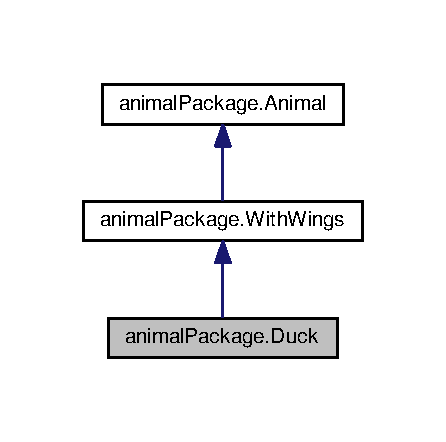
\includegraphics[width=214pt]{classanimal_package_1_1_duck__inherit__graph}
\end{center}
\end{figure}


Collaboration diagram for animal\+Package.\+Duck\+:\nopagebreak
\begin{figure}[H]
\begin{center}
\leavevmode
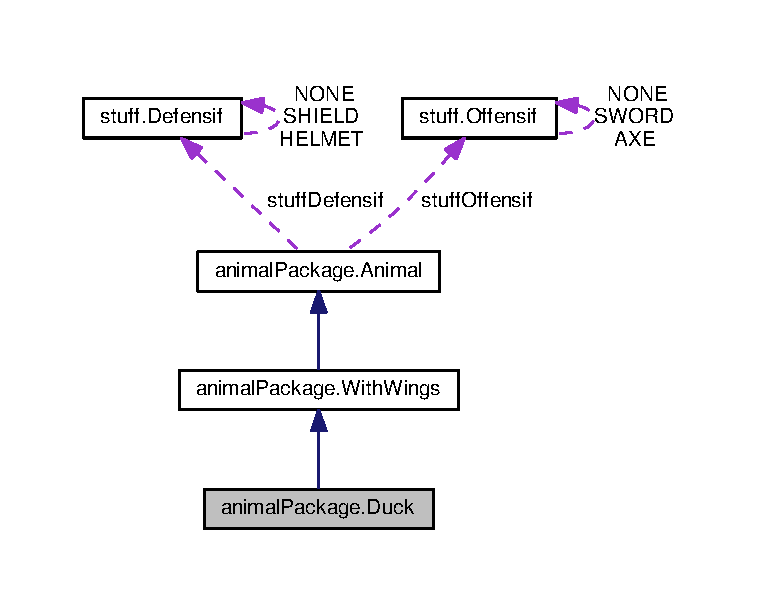
\includegraphics[width=350pt]{classanimal_package_1_1_duck__coll__graph}
\end{center}
\end{figure}
\subsection*{Public Member Functions}
\begin{DoxyCompactItemize}
\item 
\hyperlink{classanimal_package_1_1_duck_a4c98190f59b8917b2484c8854be7a2bd}{Duck} (String new\+Pseudo)
\item 
\hyperlink{classanimal_package_1_1_duck_a2d03044470b67aa9b15196300665e426}{Duck} (String new\+Pseudo, String new\+Color)
\item 
void \hyperlink{classanimal_package_1_1_duck_aeecb763501418df5ea688eca38bf7fff}{attack} (\hyperlink{classanimal_package_1_1_animal}{Animal} attacked\+Animal)
\item 
String \hyperlink{classanimal_package_1_1_duck_aff310b1799c52fc896b68de516e5d15f}{special\+Action} (\hyperlink{classanimal_package_1_1_animal}{Animal} attacked\+Animal)
\item 
void \hyperlink{classanimal_package_1_1_duck_a045c6f792ed666f372c8ae5309cfbeeb}{scream} ()
\end{DoxyCompactItemize}
\subsection*{Additional Inherited Members}


\subsection{Detailed Description}
===== Class \hyperlink{classanimal_package_1_1_duck}{Duck} =====

\begin{DoxyAuthor}{Author}
Vincent Reynaert, Nicolas Sobczak 
\end{DoxyAuthor}
\begin{DoxyVersion}{Version}
1.\+03, 11/2016 
\end{DoxyVersion}


\subsection{Constructor \& Destructor Documentation}
\index{animal\+Package\+::\+Duck@{animal\+Package\+::\+Duck}!Duck@{Duck}}
\index{Duck@{Duck}!animal\+Package\+::\+Duck@{animal\+Package\+::\+Duck}}
\subsubsection[{\texorpdfstring{Duck(\+String new\+Pseudo)}{Duck(String newPseudo)}}]{\setlength{\rightskip}{0pt plus 5cm}animal\+Package.\+Duck.\+Duck (
\begin{DoxyParamCaption}
\item[{String}]{new\+Pseudo}
\end{DoxyParamCaption}
)}\hypertarget{classanimal_package_1_1_duck_a4c98190f59b8917b2484c8854be7a2bd}{}\label{classanimal_package_1_1_duck_a4c98190f59b8917b2484c8854be7a2bd}
Constructor


\begin{DoxyParams}{Parameters}
{\em 1} & String = duck\textquotesingle{}s Pseudo \\
\hline
\end{DoxyParams}
\index{animal\+Package\+::\+Duck@{animal\+Package\+::\+Duck}!Duck@{Duck}}
\index{Duck@{Duck}!animal\+Package\+::\+Duck@{animal\+Package\+::\+Duck}}
\subsubsection[{\texorpdfstring{Duck(\+String new\+Pseudo, String new\+Color)}{Duck(String newPseudo, String newColor)}}]{\setlength{\rightskip}{0pt plus 5cm}animal\+Package.\+Duck.\+Duck (
\begin{DoxyParamCaption}
\item[{String}]{new\+Pseudo, }
\item[{String}]{new\+Color}
\end{DoxyParamCaption}
)}\hypertarget{classanimal_package_1_1_duck_a2d03044470b67aa9b15196300665e426}{}\label{classanimal_package_1_1_duck_a2d03044470b67aa9b15196300665e426}
Constructor


\begin{DoxyParams}{Parameters}
{\em 1} & String = duck\textquotesingle{}s Pseudo \\
\hline
{\em 1} & String = duck\textquotesingle{}s color \\
\hline
\end{DoxyParams}


\subsection{Member Function Documentation}
\index{animal\+Package\+::\+Duck@{animal\+Package\+::\+Duck}!attack@{attack}}
\index{attack@{attack}!animal\+Package\+::\+Duck@{animal\+Package\+::\+Duck}}
\subsubsection[{\texorpdfstring{attack(\+Animal attacked\+Animal)}{attack(Animal attackedAnimal)}}]{\setlength{\rightskip}{0pt plus 5cm}void animal\+Package.\+Duck.\+attack (
\begin{DoxyParamCaption}
\item[{{\bf Animal}}]{attacked\+Animal}
\end{DoxyParamCaption}
)}\hypertarget{classanimal_package_1_1_duck_aeecb763501418df5ea688eca38bf7fff}{}\label{classanimal_package_1_1_duck_aeecb763501418df5ea688eca38bf7fff}
attack \+: function which executes a basic attack


\begin{DoxyParams}{Parameters}
{\em \hyperlink{classanimal_package_1_1_animal}{Animal}} & attacked\+Animal \\
\hline
\end{DoxyParams}
\index{animal\+Package\+::\+Duck@{animal\+Package\+::\+Duck}!scream@{scream}}
\index{scream@{scream}!animal\+Package\+::\+Duck@{animal\+Package\+::\+Duck}}
\subsubsection[{\texorpdfstring{scream()}{scream()}}]{\setlength{\rightskip}{0pt plus 5cm}void animal\+Package.\+Duck.\+scream (
\begin{DoxyParamCaption}
{}
\end{DoxyParamCaption}
)}\hypertarget{classanimal_package_1_1_duck_a045c6f792ed666f372c8ae5309cfbeeb}{}\label{classanimal_package_1_1_duck_a045c6f792ed666f372c8ae5309cfbeeb}
scream \+: function which makes the animal scream \index{animal\+Package\+::\+Duck@{animal\+Package\+::\+Duck}!special\+Action@{special\+Action}}
\index{special\+Action@{special\+Action}!animal\+Package\+::\+Duck@{animal\+Package\+::\+Duck}}
\subsubsection[{\texorpdfstring{special\+Action(\+Animal attacked\+Animal)}{specialAction(Animal attackedAnimal)}}]{\setlength{\rightskip}{0pt plus 5cm}String animal\+Package.\+Duck.\+special\+Action (
\begin{DoxyParamCaption}
\item[{{\bf Animal}}]{attacked\+Animal}
\end{DoxyParamCaption}
)}\hypertarget{classanimal_package_1_1_duck_aff310b1799c52fc896b68de516e5d15f}{}\label{classanimal_package_1_1_duck_aff310b1799c52fc896b68de516e5d15f}
special\+Action \+: function which executes a special attack


\begin{DoxyParams}{Parameters}
{\em \hyperlink{classanimal_package_1_1_animal}{Animal}} & attacked\+Animal \\
\hline
\end{DoxyParams}
\begin{DoxyReturn}{Returns}
String 
\end{DoxyReturn}


The documentation for this class was generated from the following file\+:\begin{DoxyCompactItemize}
\item 
src/animal\+Package/Duck.\+java\end{DoxyCompactItemize}

\hypertarget{interfacespace_pig_fighter_package_1_1_execution_interface}{}\section{space\+Pig\+Fighter\+Package.\+Execution\+Interface Interface Reference}
\label{interfacespace_pig_fighter_package_1_1_execution_interface}\index{space\+Pig\+Fighter\+Package.\+Execution\+Interface@{space\+Pig\+Fighter\+Package.\+Execution\+Interface}}


Inheritance diagram for space\+Pig\+Fighter\+Package.\+Execution\+Interface\+:\nopagebreak
\begin{figure}[H]
\begin{center}
\leavevmode
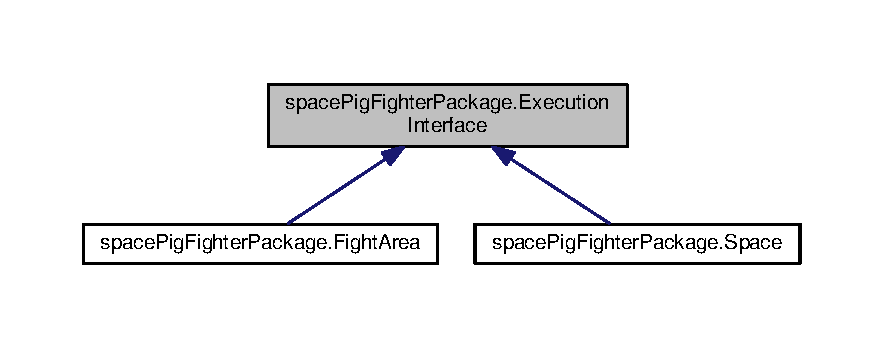
\includegraphics[width=350pt]{interfacespace_pig_fighter_package_1_1_execution_interface__inherit__graph}
\end{center}
\end{figure}
\subsection*{Public Member Functions}
\begin{DoxyCompactItemize}
\item 
String {\bfseries run} ()\hypertarget{interfacespace_pig_fighter_package_1_1_execution_interface_abd2b9509aa108fbd0f82b81b5abcd100}{}\label{interfacespace_pig_fighter_package_1_1_execution_interface_abd2b9509aa108fbd0f82b81b5abcd100}

\end{DoxyCompactItemize}


\subsection{Detailed Description}
===== interface \hyperlink{interfacespace_pig_fighter_package_1_1_execution_interface}{Execution\+Interface} =====

\begin{DoxyAuthor}{Author}
Vincent Reynaert, Nicolas Sobczak 
\end{DoxyAuthor}
\begin{DoxyVersion}{Version}
1.\+01, 11/2016 
\end{DoxyVersion}


The documentation for this interface was generated from the following file\+:\begin{DoxyCompactItemize}
\item 
src/space\+Pig\+Fighter\+Package/Execution\+Interface.\+java\end{DoxyCompactItemize}

\hypertarget{classspace_pig_fighter_package_1_1_fight_area}{}\section{space\+Pig\+Fighter\+Package.\+Fight\+Area Class Reference}
\label{classspace_pig_fighter_package_1_1_fight_area}\index{space\+Pig\+Fighter\+Package.\+Fight\+Area@{space\+Pig\+Fighter\+Package.\+Fight\+Area}}


Inheritance diagram for space\+Pig\+Fighter\+Package.\+Fight\+Area\+:\nopagebreak
\begin{figure}[H]
\begin{center}
\leavevmode
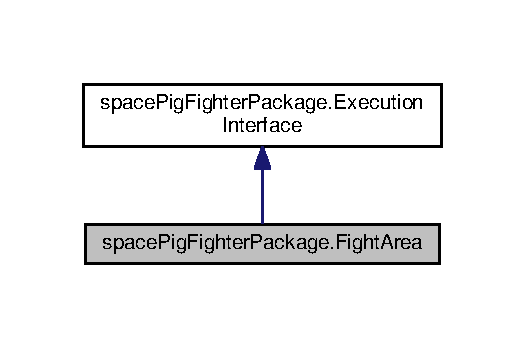
\includegraphics[width=252pt]{classspace_pig_fighter_package_1_1_fight_area__inherit__graph}
\end{center}
\end{figure}


Collaboration diagram for space\+Pig\+Fighter\+Package.\+Fight\+Area\+:\nopagebreak
\begin{figure}[H]
\begin{center}
\leavevmode
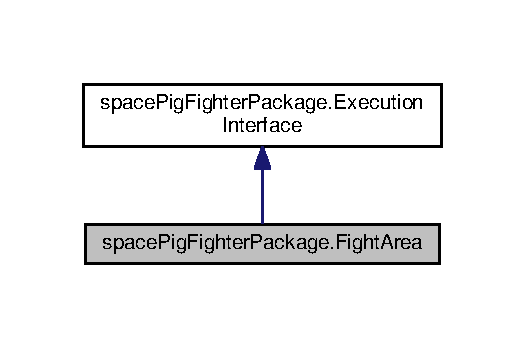
\includegraphics[width=252pt]{classspace_pig_fighter_package_1_1_fight_area__coll__graph}
\end{center}
\end{figure}
\subsection*{Public Member Functions}
\begin{DoxyCompactItemize}
\item 
\hyperlink{classspace_pig_fighter_package_1_1_fight_area_a82eab1ab77303790870fa0a866ca8c0f}{Fight\+Area} (\hyperlink{classplayer_package_1_1_player}{Player} player\+\_\+01, \hyperlink{classplayer_package_1_1_player}{Player} player\+\_\+02)
\item 
\hyperlink{classanimal_package_1_1_animal}{Animal} \hyperlink{classspace_pig_fighter_package_1_1_fight_area_a6464a4f6d21ab6ebc940ac6286e4af46}{get\+Animal\+Player01} ()
\item 
\hyperlink{classanimal_package_1_1_animal}{Animal} \hyperlink{classspace_pig_fighter_package_1_1_fight_area_a6850916669ee6860d0ea713088e7d0cb}{get\+Animal\+Player02} ()
\item 
void \hyperlink{classspace_pig_fighter_package_1_1_fight_area_a3300b7e6808c05808e244e0bcb901dad}{set\+Animal\+Player01} (\hyperlink{classanimal_package_1_1_animal}{Animal} new\+\_\+animal\+\_\+player\+\_\+01)
\item 
void \hyperlink{classspace_pig_fighter_package_1_1_fight_area_ae08c2c294e047a0eb19462baece03f17}{set\+Animal\+Player02} (\hyperlink{classanimal_package_1_1_animal}{Animal} new\+\_\+animal\+\_\+player\+\_\+02)
\item 
String \hyperlink{classspace_pig_fighter_package_1_1_fight_area_a8572396ce29c01859157b72c581fc19c}{run} ()
\end{DoxyCompactItemize}


\subsection{Detailed Description}
===== Class \hyperlink{classspace_pig_fighter_package_1_1_fight_area}{Fight\+Area} =====

\begin{DoxyAuthor}{Author}
Vincent Reynaert, Nicolas Sobczak 
\end{DoxyAuthor}
\begin{DoxyVersion}{Version}
1.\+05, 11/2016 
\end{DoxyVersion}


\subsection{Constructor \& Destructor Documentation}
\index{space\+Pig\+Fighter\+Package\+::\+Fight\+Area@{space\+Pig\+Fighter\+Package\+::\+Fight\+Area}!Fight\+Area@{Fight\+Area}}
\index{Fight\+Area@{Fight\+Area}!space\+Pig\+Fighter\+Package\+::\+Fight\+Area@{space\+Pig\+Fighter\+Package\+::\+Fight\+Area}}
\subsubsection[{\texorpdfstring{Fight\+Area(\+Player player\+\_\+01, Player player\+\_\+02)}{FightArea(Player player_01, Player player_02)}}]{\setlength{\rightskip}{0pt plus 5cm}space\+Pig\+Fighter\+Package.\+Fight\+Area.\+Fight\+Area (
\begin{DoxyParamCaption}
\item[{{\bf Player}}]{player\+\_\+01, }
\item[{{\bf Player}}]{player\+\_\+02}
\end{DoxyParamCaption}
)}\hypertarget{classspace_pig_fighter_package_1_1_fight_area_a82eab1ab77303790870fa0a866ca8c0f}{}\label{classspace_pig_fighter_package_1_1_fight_area_a82eab1ab77303790870fa0a866ca8c0f}
Constructor


\begin{DoxyParams}{Parameters}
{\em 1} & Player = player\+\_\+01 \\
\hline
{\em 1} & Player = player\+\_\+02 \\
\hline
\end{DoxyParams}


\subsection{Member Function Documentation}
\index{space\+Pig\+Fighter\+Package\+::\+Fight\+Area@{space\+Pig\+Fighter\+Package\+::\+Fight\+Area}!get\+Animal\+Player01@{get\+Animal\+Player01}}
\index{get\+Animal\+Player01@{get\+Animal\+Player01}!space\+Pig\+Fighter\+Package\+::\+Fight\+Area@{space\+Pig\+Fighter\+Package\+::\+Fight\+Area}}
\subsubsection[{\texorpdfstring{get\+Animal\+Player01()}{getAnimalPlayer01()}}]{\setlength{\rightskip}{0pt plus 5cm}{\bf Animal} space\+Pig\+Fighter\+Package.\+Fight\+Area.\+get\+Animal\+Player01 (
\begin{DoxyParamCaption}
{}
\end{DoxyParamCaption}
)}\hypertarget{classspace_pig_fighter_package_1_1_fight_area_a6464a4f6d21ab6ebc940ac6286e4af46}{}\label{classspace_pig_fighter_package_1_1_fight_area_a6464a4f6d21ab6ebc940ac6286e4af46}
Get Fighte\+Area animal\+\_\+player\+\_\+01

\begin{DoxyReturn}{Returns}
Animal animal\+\_\+player\+\_\+01 
\end{DoxyReturn}
\index{space\+Pig\+Fighter\+Package\+::\+Fight\+Area@{space\+Pig\+Fighter\+Package\+::\+Fight\+Area}!get\+Animal\+Player02@{get\+Animal\+Player02}}
\index{get\+Animal\+Player02@{get\+Animal\+Player02}!space\+Pig\+Fighter\+Package\+::\+Fight\+Area@{space\+Pig\+Fighter\+Package\+::\+Fight\+Area}}
\subsubsection[{\texorpdfstring{get\+Animal\+Player02()}{getAnimalPlayer02()}}]{\setlength{\rightskip}{0pt plus 5cm}{\bf Animal} space\+Pig\+Fighter\+Package.\+Fight\+Area.\+get\+Animal\+Player02 (
\begin{DoxyParamCaption}
{}
\end{DoxyParamCaption}
)}\hypertarget{classspace_pig_fighter_package_1_1_fight_area_a6850916669ee6860d0ea713088e7d0cb}{}\label{classspace_pig_fighter_package_1_1_fight_area_a6850916669ee6860d0ea713088e7d0cb}
Get Fighte\+Area animal\+\_\+player\+\_\+02

\begin{DoxyReturn}{Returns}
Animal animal\+\_\+player\+\_\+02 
\end{DoxyReturn}
\index{space\+Pig\+Fighter\+Package\+::\+Fight\+Area@{space\+Pig\+Fighter\+Package\+::\+Fight\+Area}!run@{run}}
\index{run@{run}!space\+Pig\+Fighter\+Package\+::\+Fight\+Area@{space\+Pig\+Fighter\+Package\+::\+Fight\+Area}}
\subsubsection[{\texorpdfstring{run()}{run()}}]{\setlength{\rightskip}{0pt plus 5cm}String space\+Pig\+Fighter\+Package.\+Fight\+Area.\+run (
\begin{DoxyParamCaption}
{}
\end{DoxyParamCaption}
)}\hypertarget{classspace_pig_fighter_package_1_1_fight_area_a8572396ce29c01859157b72c581fc19c}{}\label{classspace_pig_fighter_package_1_1_fight_area_a8572396ce29c01859157b72c581fc19c}
\hyperlink{classspace_pig_fighter_package_1_1_fight_area_a8572396ce29c01859157b72c581fc19c}{run()} \+: function which gives the result 

Implements \hyperlink{interfacespace_pig_fighter_package_1_1_execution_interface}{space\+Pig\+Fighter\+Package.\+Execution\+Interface}.

\index{space\+Pig\+Fighter\+Package\+::\+Fight\+Area@{space\+Pig\+Fighter\+Package\+::\+Fight\+Area}!set\+Animal\+Player01@{set\+Animal\+Player01}}
\index{set\+Animal\+Player01@{set\+Animal\+Player01}!space\+Pig\+Fighter\+Package\+::\+Fight\+Area@{space\+Pig\+Fighter\+Package\+::\+Fight\+Area}}
\subsubsection[{\texorpdfstring{set\+Animal\+Player01(\+Animal new\+\_\+animal\+\_\+player\+\_\+01)}{setAnimalPlayer01(Animal new_animal_player_01)}}]{\setlength{\rightskip}{0pt plus 5cm}void space\+Pig\+Fighter\+Package.\+Fight\+Area.\+set\+Animal\+Player01 (
\begin{DoxyParamCaption}
\item[{{\bf Animal}}]{new\+\_\+animal\+\_\+player\+\_\+01}
\end{DoxyParamCaption}
)}\hypertarget{classspace_pig_fighter_package_1_1_fight_area_a3300b7e6808c05808e244e0bcb901dad}{}\label{classspace_pig_fighter_package_1_1_fight_area_a3300b7e6808c05808e244e0bcb901dad}
Set Fighte\+Area animal\+\_\+player\+\_\+01


\begin{DoxyParams}{Parameters}
{\em Animal} & new\+\_\+animal\+\_\+player\+\_\+01 \\
\hline
\end{DoxyParams}
\index{space\+Pig\+Fighter\+Package\+::\+Fight\+Area@{space\+Pig\+Fighter\+Package\+::\+Fight\+Area}!set\+Animal\+Player02@{set\+Animal\+Player02}}
\index{set\+Animal\+Player02@{set\+Animal\+Player02}!space\+Pig\+Fighter\+Package\+::\+Fight\+Area@{space\+Pig\+Fighter\+Package\+::\+Fight\+Area}}
\subsubsection[{\texorpdfstring{set\+Animal\+Player02(\+Animal new\+\_\+animal\+\_\+player\+\_\+02)}{setAnimalPlayer02(Animal new_animal_player_02)}}]{\setlength{\rightskip}{0pt plus 5cm}void space\+Pig\+Fighter\+Package.\+Fight\+Area.\+set\+Animal\+Player02 (
\begin{DoxyParamCaption}
\item[{{\bf Animal}}]{new\+\_\+animal\+\_\+player\+\_\+02}
\end{DoxyParamCaption}
)}\hypertarget{classspace_pig_fighter_package_1_1_fight_area_ae08c2c294e047a0eb19462baece03f17}{}\label{classspace_pig_fighter_package_1_1_fight_area_ae08c2c294e047a0eb19462baece03f17}
Set Fighte\+Area animal\+\_\+player\+\_\+02


\begin{DoxyParams}{Parameters}
{\em Animal} & new\+\_\+animal\+\_\+player\+\_\+02 \\
\hline
\end{DoxyParams}


The documentation for this class was generated from the following file\+:\begin{DoxyCompactItemize}
\item 
src/space\+Pig\+Fighter\+Package/Fight\+Area.\+java\end{DoxyCompactItemize}

\hypertarget{classfile_management_package_1_1_file_management}{}\section{file\+Management\+Package.\+File\+Management Class Reference}
\label{classfile_management_package_1_1_file_management}\index{file\+Management\+Package.\+File\+Management@{file\+Management\+Package.\+File\+Management}}
\subsection*{Static Public Member Functions}
\begin{DoxyCompactItemize}
\item 
static void \hyperlink{classfile_management_package_1_1_file_management_ad3a42063ba99652ab0e8d8c1dfb49e3f}{create\+File} (String file\+Name)
\item 
static void \hyperlink{classfile_management_package_1_1_file_management_a70b71f4b284159b6260371e9bf59e223}{write\+File} (String file\+Name, String string\+To\+Write)
\item 
static String \hyperlink{classfile_management_package_1_1_file_management_ac41c76736949f19bd6b2b5f862211805}{write\+Story} (\hyperlink{classplayer_package_1_1_player}{Player} player\+\_\+1, \hyperlink{classplayer_package_1_1_player}{Player} player\+\_\+2, String fight\+Result)
\end{DoxyCompactItemize}


\subsection{Detailed Description}
===== Class \hyperlink{classfile_management_package_1_1_file_management}{File\+Management} =====

\begin{DoxyAuthor}{Author}
Vincent Reynaert, Nicolas Sobczak 
\end{DoxyAuthor}
\begin{DoxyVersion}{Version}
1.\+03, 11/2016 
\end{DoxyVersion}


\subsection{Member Function Documentation}
\index{file\+Management\+Package\+::\+File\+Management@{file\+Management\+Package\+::\+File\+Management}!create\+File@{create\+File}}
\index{create\+File@{create\+File}!file\+Management\+Package\+::\+File\+Management@{file\+Management\+Package\+::\+File\+Management}}
\subsubsection[{\texorpdfstring{create\+File(\+String file\+Name)}{createFile(String fileName)}}]{\setlength{\rightskip}{0pt plus 5cm}static void file\+Management\+Package.\+File\+Management.\+create\+File (
\begin{DoxyParamCaption}
\item[{String}]{file\+Name}
\end{DoxyParamCaption}
)\hspace{0.3cm}{\ttfamily [static]}}\hypertarget{classfile_management_package_1_1_file_management_ad3a42063ba99652ab0e8d8c1dfb49e3f}{}\label{classfile_management_package_1_1_file_management_ad3a42063ba99652ab0e8d8c1dfb49e3f}
create\+File function that create a file


\begin{DoxyParams}{Parameters}
{\em 1} & String file\+Name \\
\hline
\end{DoxyParams}
\index{file\+Management\+Package\+::\+File\+Management@{file\+Management\+Package\+::\+File\+Management}!write\+File@{write\+File}}
\index{write\+File@{write\+File}!file\+Management\+Package\+::\+File\+Management@{file\+Management\+Package\+::\+File\+Management}}
\subsubsection[{\texorpdfstring{write\+File(\+String file\+Name, String string\+To\+Write)}{writeFile(String fileName, String stringToWrite)}}]{\setlength{\rightskip}{0pt plus 5cm}static void file\+Management\+Package.\+File\+Management.\+write\+File (
\begin{DoxyParamCaption}
\item[{String}]{file\+Name, }
\item[{String}]{string\+To\+Write}
\end{DoxyParamCaption}
)\hspace{0.3cm}{\ttfamily [static]}}\hypertarget{classfile_management_package_1_1_file_management_a70b71f4b284159b6260371e9bf59e223}{}\label{classfile_management_package_1_1_file_management_a70b71f4b284159b6260371e9bf59e223}
write\+File function


\begin{DoxyParams}{Parameters}
{\em 1} & String file\+Name \\
\hline
{\em 1} & String string\+To\+Write \\
\hline
\end{DoxyParams}
\index{file\+Management\+Package\+::\+File\+Management@{file\+Management\+Package\+::\+File\+Management}!write\+Story@{write\+Story}}
\index{write\+Story@{write\+Story}!file\+Management\+Package\+::\+File\+Management@{file\+Management\+Package\+::\+File\+Management}}
\subsubsection[{\texorpdfstring{write\+Story(\+Player player\+\_\+1, Player player\+\_\+2, String fight\+Result)}{writeStory(Player player_1, Player player_2, String fightResult)}}]{\setlength{\rightskip}{0pt plus 5cm}static String file\+Management\+Package.\+File\+Management.\+write\+Story (
\begin{DoxyParamCaption}
\item[{{\bf Player}}]{player\+\_\+1, }
\item[{{\bf Player}}]{player\+\_\+2, }
\item[{String}]{fight\+Result}
\end{DoxyParamCaption}
)\hspace{0.3cm}{\ttfamily [static]}}\hypertarget{classfile_management_package_1_1_file_management_ac41c76736949f19bd6b2b5f862211805}{}\label{classfile_management_package_1_1_file_management_ac41c76736949f19bd6b2b5f862211805}
write\+Story function which writes the fight story


\begin{DoxyParams}{Parameters}
{\em 2} & Player player\+\_\+1 and player\+\_\+2 \\
\hline
{\em 1} & String fight\+Result \+: the result of the fight\+Area fight \\
\hline
\end{DoxyParams}


The documentation for this class was generated from the following file\+:\begin{DoxyCompactItemize}
\item 
src/file\+Management\+Package/File\+Management.\+java\end{DoxyCompactItemize}

\hypertarget{classspace_pig_fighter_package_1_1_main}{}\section{space\+Pig\+Fighter\+Package.\+Main Class Reference}
\label{classspace_pig_fighter_package_1_1_main}\index{space\+Pig\+Fighter\+Package.\+Main@{space\+Pig\+Fighter\+Package.\+Main}}
\subsection*{Static Public Member Functions}
\begin{DoxyCompactItemize}
\item 
static \hyperlink{classplayer_package_1_1_player}{Player} \hyperlink{classspace_pig_fighter_package_1_1_main_a8db9557406db889675ae060fb9c15c50}{player\+Creation} ()
\item 
static String \hyperlink{classspace_pig_fighter_package_1_1_main_a51384377791f5184a8d67188008d9007}{part\+\_\+1} (\hyperlink{classplayer_package_1_1_player}{Player} player\+\_\+1, \hyperlink{classplayer_package_1_1_player}{Player} player\+\_\+2)
\item 
static String \hyperlink{classspace_pig_fighter_package_1_1_main_a486c5dee27254957f78a4900d318b883}{part\+\_\+2} (\hyperlink{classplayer_package_1_1_player}{Player} player\+\_\+1, \hyperlink{classplayer_package_1_1_player}{Player} player\+\_\+2)
\item 
static void \hyperlink{classspace_pig_fighter_package_1_1_main_aa08fce3143ed981c78dd68d54db056a8}{main} (String\mbox{[}$\,$\mbox{]} args)
\end{DoxyCompactItemize}


\subsection{Detailed Description}
===== Class \hyperlink{classspace_pig_fighter_package_1_1_main}{Main} =====

\begin{DoxyAuthor}{Author}
Vincent Reynaert, Nicolas Sobczak 
\end{DoxyAuthor}
\begin{DoxyVersion}{Version}
1.\+01, 10/2016 
\end{DoxyVersion}


\subsection{Member Function Documentation}
\index{space\+Pig\+Fighter\+Package\+::\+Main@{space\+Pig\+Fighter\+Package\+::\+Main}!main@{main}}
\index{main@{main}!space\+Pig\+Fighter\+Package\+::\+Main@{space\+Pig\+Fighter\+Package\+::\+Main}}
\subsubsection[{\texorpdfstring{main(\+String[] args)}{main(String[] args)}}]{\setlength{\rightskip}{0pt plus 5cm}static void space\+Pig\+Fighter\+Package.\+Main.\+main (
\begin{DoxyParamCaption}
\item[{String\mbox{[}$\,$\mbox{]}}]{args}
\end{DoxyParamCaption}
)\hspace{0.3cm}{\ttfamily [static]}}\hypertarget{classspace_pig_fighter_package_1_1_main_aa08fce3143ed981c78dd68d54db056a8}{}\label{classspace_pig_fighter_package_1_1_main_aa08fce3143ed981c78dd68d54db056a8}


 main function


\begin{DoxyParams}{Parameters}
{\em 1} & String\mbox{[}\mbox{]} = args \\
\hline
\end{DoxyParams}
\index{space\+Pig\+Fighter\+Package\+::\+Main@{space\+Pig\+Fighter\+Package\+::\+Main}!part\+\_\+1@{part\+\_\+1}}
\index{part\+\_\+1@{part\+\_\+1}!space\+Pig\+Fighter\+Package\+::\+Main@{space\+Pig\+Fighter\+Package\+::\+Main}}
\subsubsection[{\texorpdfstring{part\+\_\+1(\+Player player\+\_\+1, Player player\+\_\+2)}{part_1(Player player_1, Player player_2)}}]{\setlength{\rightskip}{0pt plus 5cm}static String space\+Pig\+Fighter\+Package.\+Main.\+part\+\_\+1 (
\begin{DoxyParamCaption}
\item[{{\bf Player}}]{player\+\_\+1, }
\item[{{\bf Player}}]{player\+\_\+2}
\end{DoxyParamCaption}
)\hspace{0.3cm}{\ttfamily [static]}}\hypertarget{classspace_pig_fighter_package_1_1_main_a51384377791f5184a8d67188008d9007}{}\label{classspace_pig_fighter_package_1_1_main_a51384377791f5184a8d67188008d9007}
Game part 1 function


\begin{DoxyParams}{Parameters}
{\em 1} & Player = player\+\_\+1 \\
\hline
{\em 1} & Player = player\+\_\+2 \\
\hline
\end{DoxyParams}
\index{space\+Pig\+Fighter\+Package\+::\+Main@{space\+Pig\+Fighter\+Package\+::\+Main}!part\+\_\+2@{part\+\_\+2}}
\index{part\+\_\+2@{part\+\_\+2}!space\+Pig\+Fighter\+Package\+::\+Main@{space\+Pig\+Fighter\+Package\+::\+Main}}
\subsubsection[{\texorpdfstring{part\+\_\+2(\+Player player\+\_\+1, Player player\+\_\+2)}{part_2(Player player_1, Player player_2)}}]{\setlength{\rightskip}{0pt plus 5cm}static String space\+Pig\+Fighter\+Package.\+Main.\+part\+\_\+2 (
\begin{DoxyParamCaption}
\item[{{\bf Player}}]{player\+\_\+1, }
\item[{{\bf Player}}]{player\+\_\+2}
\end{DoxyParamCaption}
)\hspace{0.3cm}{\ttfamily [static]}}\hypertarget{classspace_pig_fighter_package_1_1_main_a486c5dee27254957f78a4900d318b883}{}\label{classspace_pig_fighter_package_1_1_main_a486c5dee27254957f78a4900d318b883}
Game part 2 function


\begin{DoxyParams}{Parameters}
{\em 1} & Player = player\+\_\+1 \\
\hline
{\em 1} & Player = player\+\_\+2 \\
\hline
\end{DoxyParams}
\index{space\+Pig\+Fighter\+Package\+::\+Main@{space\+Pig\+Fighter\+Package\+::\+Main}!player\+Creation@{player\+Creation}}
\index{player\+Creation@{player\+Creation}!space\+Pig\+Fighter\+Package\+::\+Main@{space\+Pig\+Fighter\+Package\+::\+Main}}
\subsubsection[{\texorpdfstring{player\+Creation()}{playerCreation()}}]{\setlength{\rightskip}{0pt plus 5cm}static {\bf Player} space\+Pig\+Fighter\+Package.\+Main.\+player\+Creation (
\begin{DoxyParamCaption}
{}
\end{DoxyParamCaption}
)\hspace{0.3cm}{\ttfamily [static]}}\hypertarget{classspace_pig_fighter_package_1_1_main_a8db9557406db889675ae060fb9c15c50}{}\label{classspace_pig_fighter_package_1_1_main_a8db9557406db889675ae060fb9c15c50}
player\+Creation function 

The documentation for this class was generated from the following file\+:\begin{DoxyCompactItemize}
\item 
src/space\+Pig\+Fighter\+Package/Main.\+java\end{DoxyCompactItemize}

\hypertarget{classspace_objects_1_1_meteorite}{}\section{space\+Objects.\+Meteorite Class Reference}
\label{classspace_objects_1_1_meteorite}\index{space\+Objects.\+Meteorite@{space\+Objects.\+Meteorite}}


Inheritance diagram for space\+Objects.\+Meteorite\+:\nopagebreak
\begin{figure}[H]
\begin{center}
\leavevmode
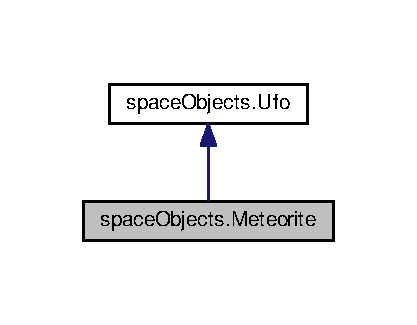
\includegraphics[width=200pt]{classspace_objects_1_1_meteorite__inherit__graph}
\end{center}
\end{figure}


Collaboration diagram for space\+Objects.\+Meteorite\+:\nopagebreak
\begin{figure}[H]
\begin{center}
\leavevmode
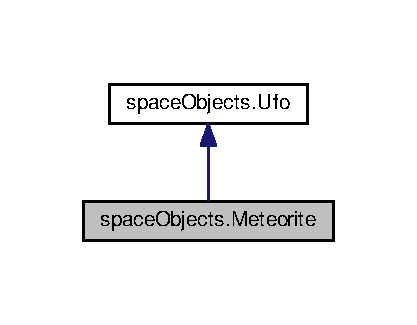
\includegraphics[width=200pt]{classspace_objects_1_1_meteorite__coll__graph}
\end{center}
\end{figure}
\subsection*{Public Member Functions}
\begin{DoxyCompactItemize}
\item 
\hyperlink{classspace_objects_1_1_meteorite_a74dda6d34c6e95af3efa73a94f143a00}{Meteorite} (\hyperlink{enumspace_objects_1_1_meteorite_size}{Meteorite\+Size} meteorite\+Size)
\item 
\hyperlink{classspace_objects_1_1_meteorite_a8bb03d9380724fb4bb4f1f4c0de69fa1}{Meteorite} (\hyperlink{enumspace_objects_1_1_positions_cube}{Positions\+Cube} position, \hyperlink{enumspace_objects_1_1_meteorite_size}{Meteorite\+Size} meteorite\+Size)
\item 
\hyperlink{enumspace_objects_1_1_meteorite_size}{Meteorite\+Size} \hyperlink{classspace_objects_1_1_meteorite_a320becfe7b60ed151c892c5300f733ca}{get\+Size} ()
\item 
void \hyperlink{classspace_objects_1_1_meteorite_af8713434bb04bc48f81784ffdea6ce3c}{set\+Size} (\hyperlink{enumspace_objects_1_1_meteorite_size}{Meteorite\+Size} new\+Size)
\end{DoxyCompactItemize}


\subsection{Detailed Description}
===== Class \hyperlink{classspace_objects_1_1_meteorite}{Meteorite} =====

\begin{DoxyAuthor}{Author}
Vincent Reynaert, Nicolas Sobczak 
\end{DoxyAuthor}
\begin{DoxyVersion}{Version}
1.\+02, 11/2016 
\end{DoxyVersion}


\subsection{Constructor \& Destructor Documentation}
\index{space\+Objects\+::\+Meteorite@{space\+Objects\+::\+Meteorite}!Meteorite@{Meteorite}}
\index{Meteorite@{Meteorite}!space\+Objects\+::\+Meteorite@{space\+Objects\+::\+Meteorite}}
\subsubsection[{\texorpdfstring{Meteorite(\+Meteorite\+Size meteorite\+Size)}{Meteorite(MeteoriteSize meteoriteSize)}}]{\setlength{\rightskip}{0pt plus 5cm}space\+Objects.\+Meteorite.\+Meteorite (
\begin{DoxyParamCaption}
\item[{{\bf Meteorite\+Size}}]{meteorite\+Size}
\end{DoxyParamCaption}
)}\hypertarget{classspace_objects_1_1_meteorite_a74dda6d34c6e95af3efa73a94f143a00}{}\label{classspace_objects_1_1_meteorite_a74dda6d34c6e95af3efa73a94f143a00}
Constructor where size is necessary selected by the player


\begin{DoxyParams}{Parameters}
{\em 1} & \hyperlink{enumspace_objects_1_1_meteorite_size}{Meteorite\+Size} = meteorite\+Size \\
\hline
\end{DoxyParams}
\index{space\+Objects\+::\+Meteorite@{space\+Objects\+::\+Meteorite}!Meteorite@{Meteorite}}
\index{Meteorite@{Meteorite}!space\+Objects\+::\+Meteorite@{space\+Objects\+::\+Meteorite}}
\subsubsection[{\texorpdfstring{Meteorite(\+Positions\+Cube position, Meteorite\+Size meteorite\+Size)}{Meteorite(PositionsCube position, MeteoriteSize meteoriteSize)}}]{\setlength{\rightskip}{0pt plus 5cm}space\+Objects.\+Meteorite.\+Meteorite (
\begin{DoxyParamCaption}
\item[{{\bf Positions\+Cube}}]{position, }
\item[{{\bf Meteorite\+Size}}]{meteorite\+Size}
\end{DoxyParamCaption}
)}\hypertarget{classspace_objects_1_1_meteorite_a8bb03d9380724fb4bb4f1f4c0de69fa1}{}\label{classspace_objects_1_1_meteorite_a8bb03d9380724fb4bb4f1f4c0de69fa1}
Constructor with selected position and size


\begin{DoxyParams}{Parameters}
{\em 1} & \hyperlink{enumspace_objects_1_1_positions_cube}{Positions\+Cube} = position \\
\hline
{\em 1} & \hyperlink{enumspace_objects_1_1_meteorite_size}{Meteorite\+Size} = meteorite\+Size \\
\hline
\end{DoxyParams}


\subsection{Member Function Documentation}
\index{space\+Objects\+::\+Meteorite@{space\+Objects\+::\+Meteorite}!get\+Size@{get\+Size}}
\index{get\+Size@{get\+Size}!space\+Objects\+::\+Meteorite@{space\+Objects\+::\+Meteorite}}
\subsubsection[{\texorpdfstring{get\+Size()}{getSize()}}]{\setlength{\rightskip}{0pt plus 5cm}{\bf Meteorite\+Size} space\+Objects.\+Meteorite.\+get\+Size (
\begin{DoxyParamCaption}
{}
\end{DoxyParamCaption}
)}\hypertarget{classspace_objects_1_1_meteorite_a320becfe7b60ed151c892c5300f733ca}{}\label{classspace_objects_1_1_meteorite_a320becfe7b60ed151c892c5300f733ca}
Get the meteorite size

\begin{DoxyReturn}{Returns}
1 \hyperlink{enumspace_objects_1_1_meteorite_size}{Meteorite\+Size} = size 
\end{DoxyReturn}
\index{space\+Objects\+::\+Meteorite@{space\+Objects\+::\+Meteorite}!set\+Size@{set\+Size}}
\index{set\+Size@{set\+Size}!space\+Objects\+::\+Meteorite@{space\+Objects\+::\+Meteorite}}
\subsubsection[{\texorpdfstring{set\+Size(\+Meteorite\+Size new\+Size)}{setSize(MeteoriteSize newSize)}}]{\setlength{\rightskip}{0pt plus 5cm}void space\+Objects.\+Meteorite.\+set\+Size (
\begin{DoxyParamCaption}
\item[{{\bf Meteorite\+Size}}]{new\+Size}
\end{DoxyParamCaption}
)}\hypertarget{classspace_objects_1_1_meteorite_af8713434bb04bc48f81784ffdea6ce3c}{}\label{classspace_objects_1_1_meteorite_af8713434bb04bc48f81784ffdea6ce3c}
Set a new size to the meteorite


\begin{DoxyParams}{Parameters}
{\em 1} & \hyperlink{enumspace_objects_1_1_meteorite_size}{Meteorite\+Size} = new\+Size \\
\hline
\end{DoxyParams}


The documentation for this class was generated from the following file\+:\begin{DoxyCompactItemize}
\item 
src/space\+Objects/Meteorite.\+java\end{DoxyCompactItemize}

\hypertarget{enumspace_objects_1_1_meteorite_size}{}\section{space\+Objects.\+Meteorite\+Size Enum Reference}
\label{enumspace_objects_1_1_meteorite_size}\index{space\+Objects.\+Meteorite\+Size@{space\+Objects.\+Meteorite\+Size}}
\subsection*{Public Attributes}
\begin{DoxyCompactItemize}
\item 
{\bfseries S\+M\+A\+LL}\hypertarget{enumspace_objects_1_1_meteorite_size_aa13610df706f2dc736c32a5159e3f7fd}{}\label{enumspace_objects_1_1_meteorite_size_aa13610df706f2dc736c32a5159e3f7fd}

\item 
{\bfseries M\+E\+D\+I\+UM}\hypertarget{enumspace_objects_1_1_meteorite_size_ae9d062e0a8f971cfe5967220562c5d71}{}\label{enumspace_objects_1_1_meteorite_size_ae9d062e0a8f971cfe5967220562c5d71}

\end{DoxyCompactItemize}


\subsection{Detailed Description}
===== Enumeration \hyperlink{enumspace_objects_1_1_meteorite_size}{Meteorite\+Size} =====

enumeration of available meteorite sizes

\begin{DoxyAuthor}{Author}
Vincent Reynaert, Nicolas Sobczak 
\end{DoxyAuthor}
\begin{DoxyVersion}{Version}
1.\+01, 10/2016 
\end{DoxyVersion}


The documentation for this enum was generated from the following file\+:\begin{DoxyCompactItemize}
\item 
src/space\+Objects/Meteorite\+Size.\+java\end{DoxyCompactItemize}

\hypertarget{classstuff_1_1_offensif}{}\section{stuff.\+Offensif Class Reference}
\label{classstuff_1_1_offensif}\index{stuff.\+Offensif@{stuff.\+Offensif}}


Collaboration diagram for stuff.\+Offensif\+:\nopagebreak
\begin{figure}[H]
\begin{center}
\leavevmode
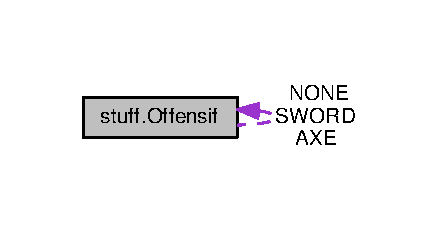
\includegraphics[width=212pt]{classstuff_1_1_offensif__coll__graph}
\end{center}
\end{figure}
\subsection*{Public Member Functions}
\begin{DoxyCompactItemize}
\item 
\hyperlink{classstuff_1_1_offensif_a84cb1366e21433f8e80c2272805fae71}{Offensif} (Integer new\+Bonus\+Value)
\item 
void \hyperlink{classstuff_1_1_offensif_abca13eb0c8696a36ae66c80c6d655902}{set\+Bonus\+Force} (Integer new\+Bonus\+Value)
\item 
Integer \hyperlink{classstuff_1_1_offensif_a263d0110fb8636758fa29eed09dba3f7}{get\+Bonus\+Force} ()
\end{DoxyCompactItemize}
\subsection*{Static Public Attributes}
\begin{DoxyCompactItemize}
\item 
static final \hyperlink{classstuff_1_1_offensif}{Offensif} \hyperlink{classstuff_1_1_offensif_a68a5dd4dd902fea924cc35f037bc0e0f}{S\+W\+O\+RD} = new \hyperlink{classstuff_1_1_offensif}{Offensif}(5)
\item 
static final \hyperlink{classstuff_1_1_offensif}{Offensif} \hyperlink{classstuff_1_1_offensif_aafe94486ee9575a68c626d86fe106bc1}{A\+XE} = new \hyperlink{classstuff_1_1_offensif}{Offensif}(10)
\item 
static final \hyperlink{classstuff_1_1_offensif}{Offensif} \hyperlink{classstuff_1_1_offensif_a48102b95df38b36febf913294ba342ae}{N\+O\+NE} = new \hyperlink{classstuff_1_1_offensif}{Offensif}(0)
\end{DoxyCompactItemize}


\subsection{Detailed Description}
===== Class \hyperlink{classstuff_1_1_offensif}{Offensif} =====

\begin{DoxyAuthor}{Author}
Vincent Reynaert, Nicolas Sobczak 
\end{DoxyAuthor}
\begin{DoxyVersion}{Version}
1.\+02, 11/2016 
\end{DoxyVersion}


\subsection{Constructor \& Destructor Documentation}
\index{stuff\+::\+Offensif@{stuff\+::\+Offensif}!Offensif@{Offensif}}
\index{Offensif@{Offensif}!stuff\+::\+Offensif@{stuff\+::\+Offensif}}
\subsubsection[{\texorpdfstring{Offensif(\+Integer new\+Bonus\+Value)}{Offensif(Integer newBonusValue)}}]{\setlength{\rightskip}{0pt plus 5cm}stuff.\+Offensif.\+Offensif (
\begin{DoxyParamCaption}
\item[{Integer}]{new\+Bonus\+Value}
\end{DoxyParamCaption}
)}\hypertarget{classstuff_1_1_offensif_a84cb1366e21433f8e80c2272805fae71}{}\label{classstuff_1_1_offensif_a84cb1366e21433f8e80c2272805fae71}
Constructor


\begin{DoxyParams}{Parameters}
{\em int} & new\+Bonus\+Value \\
\hline
\end{DoxyParams}


\subsection{Member Function Documentation}
\index{stuff\+::\+Offensif@{stuff\+::\+Offensif}!get\+Bonus\+Force@{get\+Bonus\+Force}}
\index{get\+Bonus\+Force@{get\+Bonus\+Force}!stuff\+::\+Offensif@{stuff\+::\+Offensif}}
\subsubsection[{\texorpdfstring{get\+Bonus\+Force()}{getBonusForce()}}]{\setlength{\rightskip}{0pt plus 5cm}Integer stuff.\+Offensif.\+get\+Bonus\+Force (
\begin{DoxyParamCaption}
{}
\end{DoxyParamCaption}
)}\hypertarget{classstuff_1_1_offensif_a263d0110fb8636758fa29eed09dba3f7}{}\label{classstuff_1_1_offensif_a263d0110fb8636758fa29eed09dba3f7}
Get the bonus\+Force value

\begin{DoxyReturn}{Returns}
int bonus\+Force 
\end{DoxyReturn}
\index{stuff\+::\+Offensif@{stuff\+::\+Offensif}!set\+Bonus\+Force@{set\+Bonus\+Force}}
\index{set\+Bonus\+Force@{set\+Bonus\+Force}!stuff\+::\+Offensif@{stuff\+::\+Offensif}}
\subsubsection[{\texorpdfstring{set\+Bonus\+Force(\+Integer new\+Bonus\+Value)}{setBonusForce(Integer newBonusValue)}}]{\setlength{\rightskip}{0pt plus 5cm}void stuff.\+Offensif.\+set\+Bonus\+Force (
\begin{DoxyParamCaption}
\item[{Integer}]{new\+Bonus\+Value}
\end{DoxyParamCaption}
)}\hypertarget{classstuff_1_1_offensif_abca13eb0c8696a36ae66c80c6d655902}{}\label{classstuff_1_1_offensif_abca13eb0c8696a36ae66c80c6d655902}
Set the bonus\+Force


\begin{DoxyParams}{Parameters}
{\em int} & new\+Bonus\+Value \\
\hline
\end{DoxyParams}


\subsection{Member Data Documentation}
\index{stuff\+::\+Offensif@{stuff\+::\+Offensif}!A\+XE@{A\+XE}}
\index{A\+XE@{A\+XE}!stuff\+::\+Offensif@{stuff\+::\+Offensif}}
\subsubsection[{\texorpdfstring{A\+XE}{AXE}}]{\setlength{\rightskip}{0pt plus 5cm}final {\bf Offensif} stuff.\+Offensif.\+A\+XE = new {\bf Offensif}(10)\hspace{0.3cm}{\ttfamily [static]}}\hypertarget{classstuff_1_1_offensif_aafe94486ee9575a68c626d86fe106bc1}{}\label{classstuff_1_1_offensif_aafe94486ee9575a68c626d86fe106bc1}
Increases the force of 10 \index{stuff\+::\+Offensif@{stuff\+::\+Offensif}!N\+O\+NE@{N\+O\+NE}}
\index{N\+O\+NE@{N\+O\+NE}!stuff\+::\+Offensif@{stuff\+::\+Offensif}}
\subsubsection[{\texorpdfstring{N\+O\+NE}{NONE}}]{\setlength{\rightskip}{0pt plus 5cm}final {\bf Offensif} stuff.\+Offensif.\+N\+O\+NE = new {\bf Offensif}(0)\hspace{0.3cm}{\ttfamily [static]}}\hypertarget{classstuff_1_1_offensif_a48102b95df38b36febf913294ba342ae}{}\label{classstuff_1_1_offensif_a48102b95df38b36febf913294ba342ae}
Doesn\textquotesingle{}t increase the resistance \index{stuff\+::\+Offensif@{stuff\+::\+Offensif}!S\+W\+O\+RD@{S\+W\+O\+RD}}
\index{S\+W\+O\+RD@{S\+W\+O\+RD}!stuff\+::\+Offensif@{stuff\+::\+Offensif}}
\subsubsection[{\texorpdfstring{S\+W\+O\+RD}{SWORD}}]{\setlength{\rightskip}{0pt plus 5cm}final {\bf Offensif} stuff.\+Offensif.\+S\+W\+O\+RD = new {\bf Offensif}(5)\hspace{0.3cm}{\ttfamily [static]}}\hypertarget{classstuff_1_1_offensif_a68a5dd4dd902fea924cc35f037bc0e0f}{}\label{classstuff_1_1_offensif_a68a5dd4dd902fea924cc35f037bc0e0f}
Increases the force of 5 

The documentation for this class was generated from the following file\+:\begin{DoxyCompactItemize}
\item 
src/stuff/Offensif.\+java\end{DoxyCompactItemize}

\hypertarget{classanimal_package_1_1_pig}{}\section{animal\+Package.\+Pig Class Reference}
\label{classanimal_package_1_1_pig}\index{animal\+Package.\+Pig@{animal\+Package.\+Pig}}


Inheritance diagram for animal\+Package.\+Pig\+:\nopagebreak
\begin{figure}[H]
\begin{center}
\leavevmode
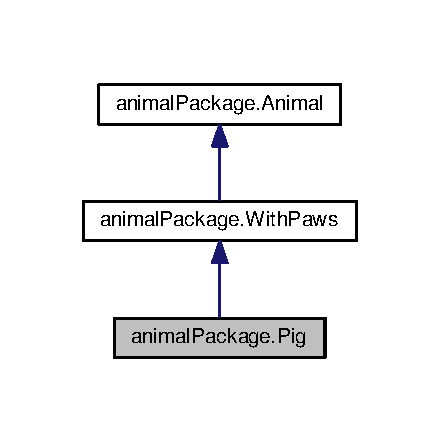
\includegraphics[width=211pt]{classanimal_package_1_1_pig__inherit__graph}
\end{center}
\end{figure}


Collaboration diagram for animal\+Package.\+Pig\+:\nopagebreak
\begin{figure}[H]
\begin{center}
\leavevmode
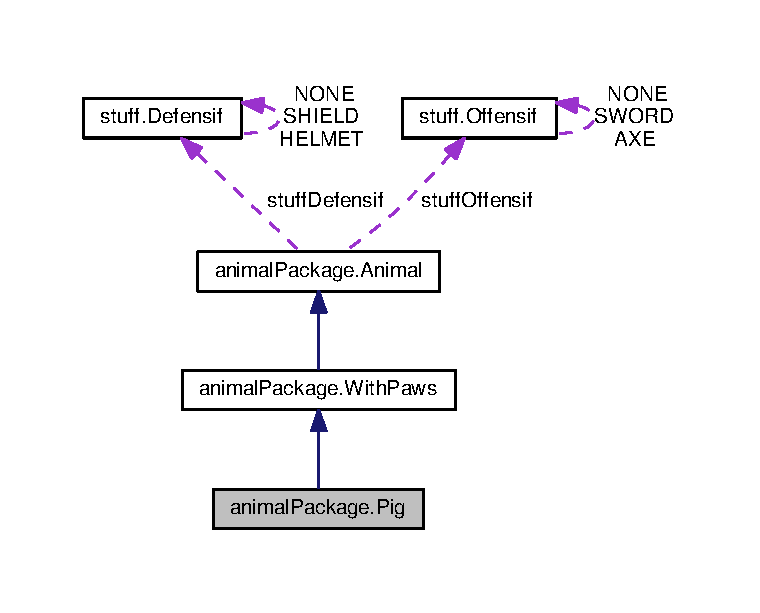
\includegraphics[width=350pt]{classanimal_package_1_1_pig__coll__graph}
\end{center}
\end{figure}
\subsection*{Public Member Functions}
\begin{DoxyCompactItemize}
\item 
\hyperlink{classanimal_package_1_1_pig_a81b2d06e31dd81ee076cf9bccfa22e17}{Pig} (String new\+Pseudo)
\item 
\hyperlink{classanimal_package_1_1_pig_a5cf5d5fef0c44a3ab8f668643ee1470b}{Pig} (String new\+Pseudo, String new\+Color)
\item 
void \hyperlink{classanimal_package_1_1_pig_a5768dcd8ec4074410cd1b6043b5fc82b}{attack} (\hyperlink{classanimal_package_1_1_animal}{Animal} attacked\+Animal)
\item 
String \hyperlink{classanimal_package_1_1_pig_aaec1dba219d9218e905d22f61ba49307}{special\+Action} (\hyperlink{classanimal_package_1_1_animal}{Animal} attacked\+Animal)
\item 
void \hyperlink{classanimal_package_1_1_pig_a9bbf1c1edfde99facac5d8871839aeef}{scream} ()
\end{DoxyCompactItemize}
\subsection*{Additional Inherited Members}


\subsection{Detailed Description}
===== Class \hyperlink{classanimal_package_1_1_pig}{Pig} =====

\begin{DoxyAuthor}{Author}
Vincent Reynaert, Nicolas Sobczak 
\end{DoxyAuthor}
\begin{DoxyVersion}{Version}
1.\+03, 11/2016 
\end{DoxyVersion}


\subsection{Constructor \& Destructor Documentation}
\index{animal\+Package\+::\+Pig@{animal\+Package\+::\+Pig}!Pig@{Pig}}
\index{Pig@{Pig}!animal\+Package\+::\+Pig@{animal\+Package\+::\+Pig}}
\subsubsection[{\texorpdfstring{Pig(\+String new\+Pseudo)}{Pig(String newPseudo)}}]{\setlength{\rightskip}{0pt plus 5cm}animal\+Package.\+Pig.\+Pig (
\begin{DoxyParamCaption}
\item[{String}]{new\+Pseudo}
\end{DoxyParamCaption}
)}\hypertarget{classanimal_package_1_1_pig_a81b2d06e31dd81ee076cf9bccfa22e17}{}\label{classanimal_package_1_1_pig_a81b2d06e31dd81ee076cf9bccfa22e17}
Constructor


\begin{DoxyParams}{Parameters}
{\em 1} & String = pig\textquotesingle{}s Pseudo \\
\hline
\end{DoxyParams}
\index{animal\+Package\+::\+Pig@{animal\+Package\+::\+Pig}!Pig@{Pig}}
\index{Pig@{Pig}!animal\+Package\+::\+Pig@{animal\+Package\+::\+Pig}}
\subsubsection[{\texorpdfstring{Pig(\+String new\+Pseudo, String new\+Color)}{Pig(String newPseudo, String newColor)}}]{\setlength{\rightskip}{0pt plus 5cm}animal\+Package.\+Pig.\+Pig (
\begin{DoxyParamCaption}
\item[{String}]{new\+Pseudo, }
\item[{String}]{new\+Color}
\end{DoxyParamCaption}
)}\hypertarget{classanimal_package_1_1_pig_a5cf5d5fef0c44a3ab8f668643ee1470b}{}\label{classanimal_package_1_1_pig_a5cf5d5fef0c44a3ab8f668643ee1470b}
Constructor


\begin{DoxyParams}{Parameters}
{\em 1} & String = pig\textquotesingle{}s Pseudo \\
\hline
{\em 1} & String = pig\textquotesingle{}s color \\
\hline
\end{DoxyParams}


\subsection{Member Function Documentation}
\index{animal\+Package\+::\+Pig@{animal\+Package\+::\+Pig}!attack@{attack}}
\index{attack@{attack}!animal\+Package\+::\+Pig@{animal\+Package\+::\+Pig}}
\subsubsection[{\texorpdfstring{attack(\+Animal attacked\+Animal)}{attack(Animal attackedAnimal)}}]{\setlength{\rightskip}{0pt plus 5cm}void animal\+Package.\+Pig.\+attack (
\begin{DoxyParamCaption}
\item[{{\bf Animal}}]{attacked\+Animal}
\end{DoxyParamCaption}
)}\hypertarget{classanimal_package_1_1_pig_a5768dcd8ec4074410cd1b6043b5fc82b}{}\label{classanimal_package_1_1_pig_a5768dcd8ec4074410cd1b6043b5fc82b}
attack \+: function which executes a basic attack


\begin{DoxyParams}{Parameters}
{\em \hyperlink{classanimal_package_1_1_animal}{Animal}} & attacked\+Animal \\
\hline
\end{DoxyParams}
\index{animal\+Package\+::\+Pig@{animal\+Package\+::\+Pig}!scream@{scream}}
\index{scream@{scream}!animal\+Package\+::\+Pig@{animal\+Package\+::\+Pig}}
\subsubsection[{\texorpdfstring{scream()}{scream()}}]{\setlength{\rightskip}{0pt plus 5cm}void animal\+Package.\+Pig.\+scream (
\begin{DoxyParamCaption}
{}
\end{DoxyParamCaption}
)}\hypertarget{classanimal_package_1_1_pig_a9bbf1c1edfde99facac5d8871839aeef}{}\label{classanimal_package_1_1_pig_a9bbf1c1edfde99facac5d8871839aeef}
scream \+: function which makes the animal scream \index{animal\+Package\+::\+Pig@{animal\+Package\+::\+Pig}!special\+Action@{special\+Action}}
\index{special\+Action@{special\+Action}!animal\+Package\+::\+Pig@{animal\+Package\+::\+Pig}}
\subsubsection[{\texorpdfstring{special\+Action(\+Animal attacked\+Animal)}{specialAction(Animal attackedAnimal)}}]{\setlength{\rightskip}{0pt plus 5cm}String animal\+Package.\+Pig.\+special\+Action (
\begin{DoxyParamCaption}
\item[{{\bf Animal}}]{attacked\+Animal}
\end{DoxyParamCaption}
)}\hypertarget{classanimal_package_1_1_pig_aaec1dba219d9218e905d22f61ba49307}{}\label{classanimal_package_1_1_pig_aaec1dba219d9218e905d22f61ba49307}
special\+Action \+: function which executes a special attack


\begin{DoxyParams}{Parameters}
{\em \hyperlink{classanimal_package_1_1_animal}{Animal}} & attacked\+Animal \\
\hline
\end{DoxyParams}
\begin{DoxyReturn}{Returns}
String 
\end{DoxyReturn}


The documentation for this class was generated from the following file\+:\begin{DoxyCompactItemize}
\item 
src/animal\+Package/Pig.\+java\end{DoxyCompactItemize}

\hypertarget{classplayer_package_1_1_player}{}\section{player\+Package.\+Player Class Reference}
\label{classplayer_package_1_1_player}\index{player\+Package.\+Player@{player\+Package.\+Player}}
\subsection*{Public Member Functions}
\begin{DoxyCompactItemize}
\item 
\hyperlink{classplayer_package_1_1_player_aff98b4fbad1a0f74315e6614626b659b}{Player} (int animal\+Class, String new\+Pseudo, String animal\+Color, String spacecraft\+Color)
\item 
\hyperlink{classanimal_package_1_1_animal}{Animal} \hyperlink{classplayer_package_1_1_player_a717b010255496ff8873966397c6d2ead}{get\+Animal} ()
\item 
\hyperlink{classspace_objects_1_1_spacecraft}{Spacecraft} \hyperlink{classplayer_package_1_1_player_a02a4b5337e6deb3be1f703a3d6b33148}{get\+Spacecraft} ()
\item 
void \hyperlink{classplayer_package_1_1_player_a68501d828837b1b6babc6fb32605feb7}{set\+Animal} (\hyperlink{classanimal_package_1_1_animal}{Animal} new\+Animal)
\item 
void \hyperlink{classplayer_package_1_1_player_ab86e253738c3f4e7930d136e3837b5c4}{set\+Spacecraft} (\hyperlink{classspace_objects_1_1_spacecraft}{Spacecraft} new\+Spacecraft)
\end{DoxyCompactItemize}


\subsection{Detailed Description}
===== Class \hyperlink{classplayer_package_1_1_player}{Player} =====

\begin{DoxyAuthor}{Author}
Vincent Reynaert, Nicolas Sobczak 
\end{DoxyAuthor}
\begin{DoxyVersion}{Version}
1.\+01, 10/2016 
\end{DoxyVersion}


\subsection{Constructor \& Destructor Documentation}
\index{player\+Package\+::\+Player@{player\+Package\+::\+Player}!Player@{Player}}
\index{Player@{Player}!player\+Package\+::\+Player@{player\+Package\+::\+Player}}
\subsubsection[{\texorpdfstring{Player(int animal\+Class, String new\+Pseudo, String animal\+Color, String spacecraft\+Color)}{Player(int animalClass, String newPseudo, String animalColor, String spacecraftColor)}}]{\setlength{\rightskip}{0pt plus 5cm}player\+Package.\+Player.\+Player (
\begin{DoxyParamCaption}
\item[{int}]{animal\+Class, }
\item[{String}]{new\+Pseudo, }
\item[{String}]{animal\+Color, }
\item[{String}]{spacecraft\+Color}
\end{DoxyParamCaption}
)}\hypertarget{classplayer_package_1_1_player_aff98b4fbad1a0f74315e6614626b659b}{}\label{classplayer_package_1_1_player_aff98b4fbad1a0f74315e6614626b659b}
Constructor with animal


\begin{DoxyParams}{Parameters}
{\em 1} & int animal\+Class \\
\hline
{\em 1} & String new\+Pseudo \\
\hline
{\em 1} & String animal\+Color \\
\hline
{\em 1} & String spacecraft\+Color \\
\hline
\end{DoxyParams}


\subsection{Member Function Documentation}
\index{player\+Package\+::\+Player@{player\+Package\+::\+Player}!get\+Animal@{get\+Animal}}
\index{get\+Animal@{get\+Animal}!player\+Package\+::\+Player@{player\+Package\+::\+Player}}
\subsubsection[{\texorpdfstring{get\+Animal()}{getAnimal()}}]{\setlength{\rightskip}{0pt plus 5cm}{\bf Animal} player\+Package.\+Player.\+get\+Animal (
\begin{DoxyParamCaption}
{}
\end{DoxyParamCaption}
)}\hypertarget{classplayer_package_1_1_player_a717b010255496ff8873966397c6d2ead}{}\label{classplayer_package_1_1_player_a717b010255496ff8873966397c6d2ead}
Get player\textquotesingle{}s animal

\begin{DoxyReturn}{Returns}
1 Animal = player\textquotesingle{}s animal 
\end{DoxyReturn}
\index{player\+Package\+::\+Player@{player\+Package\+::\+Player}!get\+Spacecraft@{get\+Spacecraft}}
\index{get\+Spacecraft@{get\+Spacecraft}!player\+Package\+::\+Player@{player\+Package\+::\+Player}}
\subsubsection[{\texorpdfstring{get\+Spacecraft()}{getSpacecraft()}}]{\setlength{\rightskip}{0pt plus 5cm}{\bf Spacecraft} player\+Package.\+Player.\+get\+Spacecraft (
\begin{DoxyParamCaption}
{}
\end{DoxyParamCaption}
)}\hypertarget{classplayer_package_1_1_player_a02a4b5337e6deb3be1f703a3d6b33148}{}\label{classplayer_package_1_1_player_a02a4b5337e6deb3be1f703a3d6b33148}
Get player\textquotesingle{}s spacecraft

\begin{DoxyReturn}{Returns}
1 Spacecraft = player\textquotesingle{}s spacecraft 
\end{DoxyReturn}
\index{player\+Package\+::\+Player@{player\+Package\+::\+Player}!set\+Animal@{set\+Animal}}
\index{set\+Animal@{set\+Animal}!player\+Package\+::\+Player@{player\+Package\+::\+Player}}
\subsubsection[{\texorpdfstring{set\+Animal(\+Animal new\+Animal)}{setAnimal(Animal newAnimal)}}]{\setlength{\rightskip}{0pt plus 5cm}void player\+Package.\+Player.\+set\+Animal (
\begin{DoxyParamCaption}
\item[{{\bf Animal}}]{new\+Animal}
\end{DoxyParamCaption}
)}\hypertarget{classplayer_package_1_1_player_a68501d828837b1b6babc6fb32605feb7}{}\label{classplayer_package_1_1_player_a68501d828837b1b6babc6fb32605feb7}
Set player\textquotesingle{}s animal


\begin{DoxyParams}{Parameters}
{\em 1} & Animal = new\+Animal \\
\hline
\end{DoxyParams}
\index{player\+Package\+::\+Player@{player\+Package\+::\+Player}!set\+Spacecraft@{set\+Spacecraft}}
\index{set\+Spacecraft@{set\+Spacecraft}!player\+Package\+::\+Player@{player\+Package\+::\+Player}}
\subsubsection[{\texorpdfstring{set\+Spacecraft(\+Spacecraft new\+Spacecraft)}{setSpacecraft(Spacecraft newSpacecraft)}}]{\setlength{\rightskip}{0pt plus 5cm}void player\+Package.\+Player.\+set\+Spacecraft (
\begin{DoxyParamCaption}
\item[{{\bf Spacecraft}}]{new\+Spacecraft}
\end{DoxyParamCaption}
)}\hypertarget{classplayer_package_1_1_player_ab86e253738c3f4e7930d136e3837b5c4}{}\label{classplayer_package_1_1_player_ab86e253738c3f4e7930d136e3837b5c4}
Set player\textquotesingle{}s spacecraft


\begin{DoxyParams}{Parameters}
{\em 1} & Spacecraft = new\+Spacecraft \\
\hline
\end{DoxyParams}


The documentation for this class was generated from the following file\+:\begin{DoxyCompactItemize}
\item 
src/player\+Package/Player.\+java\end{DoxyCompactItemize}

\hypertarget{classspace_objects_1_1_position_exception}{}\section{space\+Objects.\+Position\+Exception Class Reference}
\label{classspace_objects_1_1_position_exception}\index{space\+Objects.\+Position\+Exception@{space\+Objects.\+Position\+Exception}}


Inheritance diagram for space\+Objects.\+Position\+Exception\+:\nopagebreak
\begin{figure}[H]
\begin{center}
\leavevmode
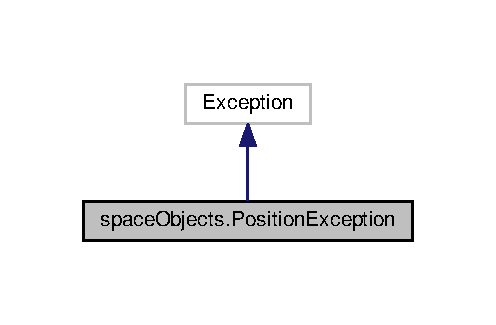
\includegraphics[width=238pt]{classspace_objects_1_1_position_exception__inherit__graph}
\end{center}
\end{figure}


Collaboration diagram for space\+Objects.\+Position\+Exception\+:\nopagebreak
\begin{figure}[H]
\begin{center}
\leavevmode
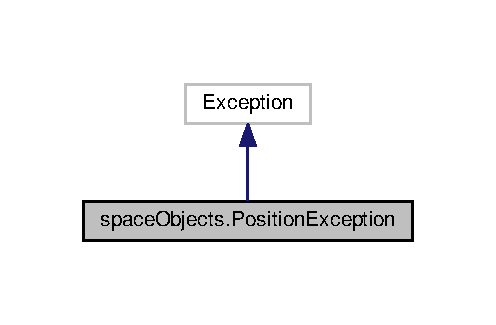
\includegraphics[width=238pt]{classspace_objects_1_1_position_exception__coll__graph}
\end{center}
\end{figure}


\subsection{Detailed Description}
===== Class \hyperlink{classspace_objects_1_1_position_exception}{Position\+Exception} =====

\begin{DoxyAuthor}{Author}
Vincent Reynaert, Nicolas Sobczak 
\end{DoxyAuthor}
\begin{DoxyVersion}{Version}
1.\+01, 11/2016 
\end{DoxyVersion}


The documentation for this class was generated from the following file\+:\begin{DoxyCompactItemize}
\item 
src/space\+Objects/Position\+Exception.\+java\end{DoxyCompactItemize}

\hypertarget{enumspace_objects_1_1_positions_cube}{}\section{space\+Objects.\+Positions\+Cube Enum Reference}
\label{enumspace_objects_1_1_positions_cube}\index{space\+Objects.\+Positions\+Cube@{space\+Objects.\+Positions\+Cube}}
\subsection*{Public Attributes}
\begin{DoxyCompactItemize}
\item 
{\bfseries N\+O\+NE}\hypertarget{enumspace_objects_1_1_positions_cube_ab013d81882824cd3f115a81d819ba99c}{}\label{enumspace_objects_1_1_positions_cube_ab013d81882824cd3f115a81d819ba99c}

\item 
{\bfseries O\+OO}\hypertarget{enumspace_objects_1_1_positions_cube_a03592a9617bca457eff42cc17169dcbe}{}\label{enumspace_objects_1_1_positions_cube_a03592a9617bca457eff42cc17169dcbe}

\item 
{\bfseries O\+OI}\hypertarget{enumspace_objects_1_1_positions_cube_ad06ca8feea253931b442c2c966136779}{}\label{enumspace_objects_1_1_positions_cube_ad06ca8feea253931b442c2c966136779}

\item 
{\bfseries O\+IO}\hypertarget{enumspace_objects_1_1_positions_cube_a855b12a06f899185a9dc815bd06ebd56}{}\label{enumspace_objects_1_1_positions_cube_a855b12a06f899185a9dc815bd06ebd56}

\item 
{\bfseries I\+OO}\hypertarget{enumspace_objects_1_1_positions_cube_a110cf046b9a973af4750627f41196169}{}\label{enumspace_objects_1_1_positions_cube_a110cf046b9a973af4750627f41196169}

\item 
{\bfseries I\+IO}\hypertarget{enumspace_objects_1_1_positions_cube_a2abbffc5a806aa1c48e780fb662a90aa}{}\label{enumspace_objects_1_1_positions_cube_a2abbffc5a806aa1c48e780fb662a90aa}

\item 
{\bfseries O\+II}\hypertarget{enumspace_objects_1_1_positions_cube_ad8ccd76124d548ac40fa7c28b276dae9}{}\label{enumspace_objects_1_1_positions_cube_ad8ccd76124d548ac40fa7c28b276dae9}

\item 
{\bfseries I\+OI}\hypertarget{enumspace_objects_1_1_positions_cube_aeacc958ccb6bcac73e8ab9455873fb79}{}\label{enumspace_objects_1_1_positions_cube_aeacc958ccb6bcac73e8ab9455873fb79}

\end{DoxyCompactItemize}


\subsection{Detailed Description}
===== Enumeration \hyperlink{enumspace_objects_1_1_meteorite_size}{Meteorite\+Size} =====

enumeration of possible positions for the \hyperlink{classspace_objects_1_1_spacecraft}{Spacecraft} in the Cube\+Environment O = 0 and I = 1

\begin{DoxyAuthor}{Author}
Vincent Reynaert, Nicolas Sobczak 
\end{DoxyAuthor}
\begin{DoxyVersion}{Version}
1.\+01, 10/2016 
\end{DoxyVersion}


The documentation for this enum was generated from the following file\+:\begin{DoxyCompactItemize}
\item 
src/space\+Objects/Positions\+Cube.\+java\end{DoxyCompactItemize}

\hypertarget{classspace_pig_fighter_package_1_1_space}{}\section{space\+Pig\+Fighter\+Package.\+Space Class Reference}
\label{classspace_pig_fighter_package_1_1_space}\index{space\+Pig\+Fighter\+Package.\+Space@{space\+Pig\+Fighter\+Package.\+Space}}


Inheritance diagram for space\+Pig\+Fighter\+Package.\+Space\+:\nopagebreak
\begin{figure}[H]
\begin{center}
\leavevmode
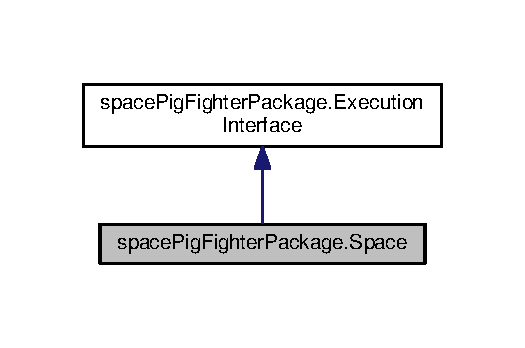
\includegraphics[width=252pt]{classspace_pig_fighter_package_1_1_space__inherit__graph}
\end{center}
\end{figure}


Collaboration diagram for space\+Pig\+Fighter\+Package.\+Space\+:\nopagebreak
\begin{figure}[H]
\begin{center}
\leavevmode
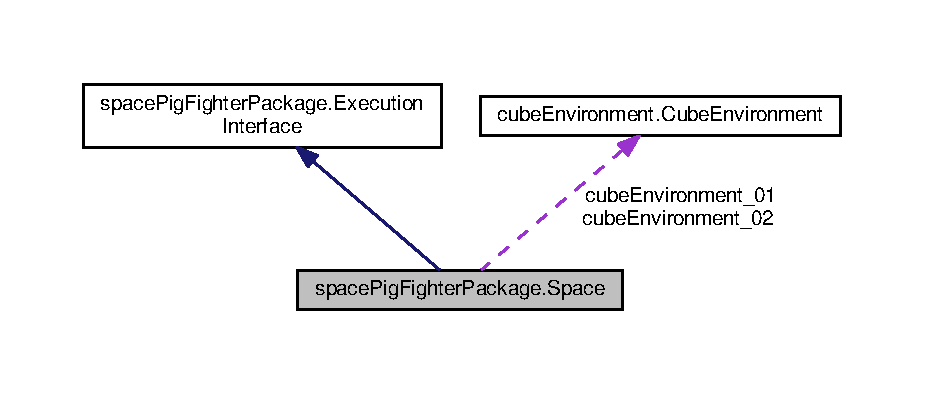
\includegraphics[width=350pt]{classspace_pig_fighter_package_1_1_space__coll__graph}
\end{center}
\end{figure}
\subsection*{Public Member Functions}
\begin{DoxyCompactItemize}
\item 
\hyperlink{classspace_pig_fighter_package_1_1_space_acc82deac40857c4b4634d1d586a953c3}{Space} (\hyperlink{classplayer_package_1_1_player}{Player} player\+\_\+1, \hyperlink{classplayer_package_1_1_player}{Player} player\+\_\+2)
\item 
\hyperlink{classcube_environment_1_1_cube_environment}{Cube\+Environment} \hyperlink{classspace_pig_fighter_package_1_1_space_a1988b77ec438cb872e6b6835346ae197}{get\+Cube\+Environment01} ()
\item 
\hyperlink{classcube_environment_1_1_cube_environment}{Cube\+Environment} \hyperlink{classspace_pig_fighter_package_1_1_space_ae4bf3ede16be09eecbf405f38a1ee265}{get\+Cube\+Environment02} ()
\item 
void \hyperlink{classspace_pig_fighter_package_1_1_space_a78fdde1cef2396b9f53954f79ddacdbf}{set\+Cube\+Environment01} (\hyperlink{classcube_environment_1_1_cube_environment}{Cube\+Environment} new\+\_\+cube\+Environment\+\_\+01)
\item 
void \hyperlink{classspace_pig_fighter_package_1_1_space_a49a1da87cb6b0905fd3aa5e2a45b39b2}{sset\+Cube\+Environment02} (\hyperlink{classcube_environment_1_1_cube_environment}{Cube\+Environment} new\+\_\+cube\+Environment\+\_\+02)
\item 
String \hyperlink{classspace_pig_fighter_package_1_1_space_ad6fdcc04d31a9b7f50fc5be0baebe71c}{run} ()
\end{DoxyCompactItemize}
\subsection*{Public Attributes}
\begin{DoxyCompactItemize}
\item 
\hyperlink{classcube_environment_1_1_cube_environment}{Cube\+Environment} {\bfseries cube\+Environment\+\_\+01}\hypertarget{classspace_pig_fighter_package_1_1_space_a1d1a8c4c70053158b0bbdf6e101e8f50}{}\label{classspace_pig_fighter_package_1_1_space_a1d1a8c4c70053158b0bbdf6e101e8f50}

\item 
\hyperlink{classcube_environment_1_1_cube_environment}{Cube\+Environment} {\bfseries cube\+Environment\+\_\+02}\hypertarget{classspace_pig_fighter_package_1_1_space_a5060ae0f965e0121658a8f305bfbe810}{}\label{classspace_pig_fighter_package_1_1_space_a5060ae0f965e0121658a8f305bfbe810}

\end{DoxyCompactItemize}


\subsection{Detailed Description}
===== Class \hyperlink{classspace_pig_fighter_package_1_1_space}{Space} =====

\begin{DoxyAuthor}{Author}
Vincent Reynaert, Nicolas Sobczak 
\end{DoxyAuthor}
\begin{DoxyVersion}{Version}
1.\+03, 11/2016 
\end{DoxyVersion}


\subsection{Constructor \& Destructor Documentation}
\index{space\+Pig\+Fighter\+Package\+::\+Space@{space\+Pig\+Fighter\+Package\+::\+Space}!Space@{Space}}
\index{Space@{Space}!space\+Pig\+Fighter\+Package\+::\+Space@{space\+Pig\+Fighter\+Package\+::\+Space}}
\subsubsection[{\texorpdfstring{Space(\+Player player\+\_\+1, Player player\+\_\+2)}{Space(Player player_1, Player player_2)}}]{\setlength{\rightskip}{0pt plus 5cm}space\+Pig\+Fighter\+Package.\+Space.\+Space (
\begin{DoxyParamCaption}
\item[{{\bf Player}}]{player\+\_\+1, }
\item[{{\bf Player}}]{player\+\_\+2}
\end{DoxyParamCaption}
)}\hypertarget{classspace_pig_fighter_package_1_1_space_acc82deac40857c4b4634d1d586a953c3}{}\label{classspace_pig_fighter_package_1_1_space_acc82deac40857c4b4634d1d586a953c3}
Constructor


\begin{DoxyParams}{Parameters}
{\em 1} & Player = player\+\_\+1 \\
\hline
{\em 1} & Player = player\+\_\+2 \\
\hline
\end{DoxyParams}


\subsection{Member Function Documentation}
\index{space\+Pig\+Fighter\+Package\+::\+Space@{space\+Pig\+Fighter\+Package\+::\+Space}!get\+Cube\+Environment01@{get\+Cube\+Environment01}}
\index{get\+Cube\+Environment01@{get\+Cube\+Environment01}!space\+Pig\+Fighter\+Package\+::\+Space@{space\+Pig\+Fighter\+Package\+::\+Space}}
\subsubsection[{\texorpdfstring{get\+Cube\+Environment01()}{getCubeEnvironment01()}}]{\setlength{\rightskip}{0pt plus 5cm}{\bf Cube\+Environment} space\+Pig\+Fighter\+Package.\+Space.\+get\+Cube\+Environment01 (
\begin{DoxyParamCaption}
{}
\end{DoxyParamCaption}
)}\hypertarget{classspace_pig_fighter_package_1_1_space_a1988b77ec438cb872e6b6835346ae197}{}\label{classspace_pig_fighter_package_1_1_space_a1988b77ec438cb872e6b6835346ae197}
Get \hyperlink{classspace_pig_fighter_package_1_1_space}{Space} cube\+Environment\+\_\+01

\begin{DoxyReturn}{Returns}
Cube\+Environment cube\+Environment\+\_\+01 
\end{DoxyReturn}
\index{space\+Pig\+Fighter\+Package\+::\+Space@{space\+Pig\+Fighter\+Package\+::\+Space}!get\+Cube\+Environment02@{get\+Cube\+Environment02}}
\index{get\+Cube\+Environment02@{get\+Cube\+Environment02}!space\+Pig\+Fighter\+Package\+::\+Space@{space\+Pig\+Fighter\+Package\+::\+Space}}
\subsubsection[{\texorpdfstring{get\+Cube\+Environment02()}{getCubeEnvironment02()}}]{\setlength{\rightskip}{0pt plus 5cm}{\bf Cube\+Environment} space\+Pig\+Fighter\+Package.\+Space.\+get\+Cube\+Environment02 (
\begin{DoxyParamCaption}
{}
\end{DoxyParamCaption}
)}\hypertarget{classspace_pig_fighter_package_1_1_space_ae4bf3ede16be09eecbf405f38a1ee265}{}\label{classspace_pig_fighter_package_1_1_space_ae4bf3ede16be09eecbf405f38a1ee265}
Get \hyperlink{classspace_pig_fighter_package_1_1_space}{Space} cube\+Environment\+\_\+02

\begin{DoxyReturn}{Returns}
Cube\+Environment cube\+Environment\+\_\+02 
\end{DoxyReturn}
\index{space\+Pig\+Fighter\+Package\+::\+Space@{space\+Pig\+Fighter\+Package\+::\+Space}!run@{run}}
\index{run@{run}!space\+Pig\+Fighter\+Package\+::\+Space@{space\+Pig\+Fighter\+Package\+::\+Space}}
\subsubsection[{\texorpdfstring{run()}{run()}}]{\setlength{\rightskip}{0pt plus 5cm}String space\+Pig\+Fighter\+Package.\+Space.\+run (
\begin{DoxyParamCaption}
{}
\end{DoxyParamCaption}
)}\hypertarget{classspace_pig_fighter_package_1_1_space_ad6fdcc04d31a9b7f50fc5be0baebe71c}{}\label{classspace_pig_fighter_package_1_1_space_ad6fdcc04d31a9b7f50fc5be0baebe71c}
\hyperlink{classspace_pig_fighter_package_1_1_space_ad6fdcc04d31a9b7f50fc5be0baebe71c}{run()} 

Implements \hyperlink{interfacespace_pig_fighter_package_1_1_execution_interface}{space\+Pig\+Fighter\+Package.\+Execution\+Interface}.

\index{space\+Pig\+Fighter\+Package\+::\+Space@{space\+Pig\+Fighter\+Package\+::\+Space}!set\+Cube\+Environment01@{set\+Cube\+Environment01}}
\index{set\+Cube\+Environment01@{set\+Cube\+Environment01}!space\+Pig\+Fighter\+Package\+::\+Space@{space\+Pig\+Fighter\+Package\+::\+Space}}
\subsubsection[{\texorpdfstring{set\+Cube\+Environment01(\+Cube\+Environment new\+\_\+cube\+Environment\+\_\+01)}{setCubeEnvironment01(CubeEnvironment new_cubeEnvironment_01)}}]{\setlength{\rightskip}{0pt plus 5cm}void space\+Pig\+Fighter\+Package.\+Space.\+set\+Cube\+Environment01 (
\begin{DoxyParamCaption}
\item[{{\bf Cube\+Environment}}]{new\+\_\+cube\+Environment\+\_\+01}
\end{DoxyParamCaption}
)}\hypertarget{classspace_pig_fighter_package_1_1_space_a78fdde1cef2396b9f53954f79ddacdbf}{}\label{classspace_pig_fighter_package_1_1_space_a78fdde1cef2396b9f53954f79ddacdbf}
Set \hyperlink{classspace_pig_fighter_package_1_1_space}{Space} cube\+Environment\+\_\+01


\begin{DoxyParams}{Parameters}
{\em Cube\+Environment} & cube\+Environment\+\_\+01 \\
\hline
\end{DoxyParams}
\index{space\+Pig\+Fighter\+Package\+::\+Space@{space\+Pig\+Fighter\+Package\+::\+Space}!sset\+Cube\+Environment02@{sset\+Cube\+Environment02}}
\index{sset\+Cube\+Environment02@{sset\+Cube\+Environment02}!space\+Pig\+Fighter\+Package\+::\+Space@{space\+Pig\+Fighter\+Package\+::\+Space}}
\subsubsection[{\texorpdfstring{sset\+Cube\+Environment02(\+Cube\+Environment new\+\_\+cube\+Environment\+\_\+02)}{ssetCubeEnvironment02(CubeEnvironment new_cubeEnvironment_02)}}]{\setlength{\rightskip}{0pt plus 5cm}void space\+Pig\+Fighter\+Package.\+Space.\+sset\+Cube\+Environment02 (
\begin{DoxyParamCaption}
\item[{{\bf Cube\+Environment}}]{new\+\_\+cube\+Environment\+\_\+02}
\end{DoxyParamCaption}
)}\hypertarget{classspace_pig_fighter_package_1_1_space_a49a1da87cb6b0905fd3aa5e2a45b39b2}{}\label{classspace_pig_fighter_package_1_1_space_a49a1da87cb6b0905fd3aa5e2a45b39b2}
Set \hyperlink{classspace_pig_fighter_package_1_1_space}{Space} cube\+Environment\+\_\+02


\begin{DoxyParams}{Parameters}
{\em Cube\+Environment} & cube\+Environment\+\_\+02 \\
\hline
\end{DoxyParams}


The documentation for this class was generated from the following file\+:\begin{DoxyCompactItemize}
\item 
src/space\+Pig\+Fighter\+Package/Space.\+java\end{DoxyCompactItemize}

\hypertarget{classspace_objects_1_1_spacecraft}{}\section{space\+Objects.\+Spacecraft Class Reference}
\label{classspace_objects_1_1_spacecraft}\index{space\+Objects.\+Spacecraft@{space\+Objects.\+Spacecraft}}


Inheritance diagram for space\+Objects.\+Spacecraft\+:\nopagebreak
\begin{figure}[H]
\begin{center}
\leavevmode
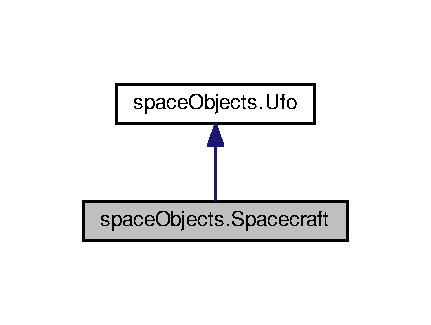
\includegraphics[width=207pt]{classspace_objects_1_1_spacecraft__inherit__graph}
\end{center}
\end{figure}


Collaboration diagram for space\+Objects.\+Spacecraft\+:\nopagebreak
\begin{figure}[H]
\begin{center}
\leavevmode
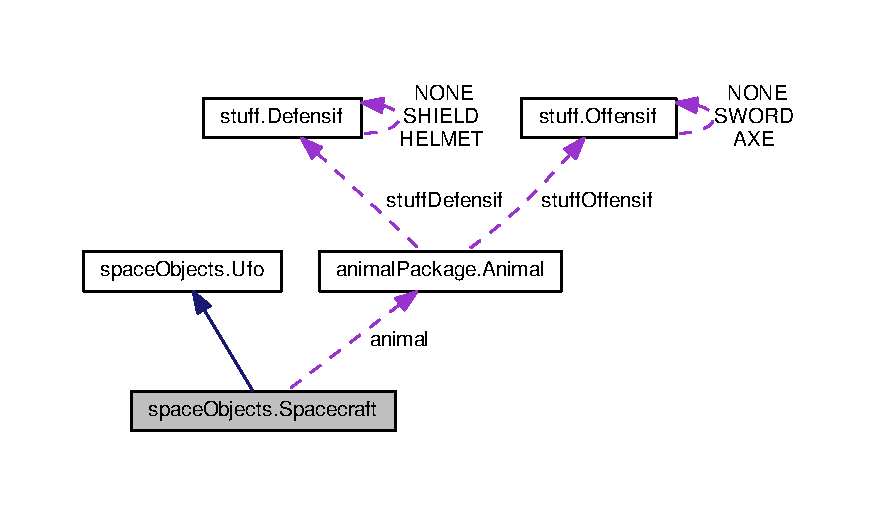
\includegraphics[width=350pt]{classspace_objects_1_1_spacecraft__coll__graph}
\end{center}
\end{figure}
\subsection*{Public Member Functions}
\begin{DoxyCompactItemize}
\item 
\hyperlink{classspace_objects_1_1_spacecraft_afc5d312686349bb5b6be07147c75a06f}{Spacecraft} ()
\item 
\hyperlink{classspace_objects_1_1_spacecraft_af56e1777de0c0971bedb3d6267a7ad47}{Spacecraft} (String color\+Name)
\item 
\hyperlink{classspace_objects_1_1_spacecraft_a807f3b576f0bf90a479abfb981436b50}{Spacecraft} (\hyperlink{classanimal_package_1_1_animal}{Animal} my\+Animal)
\item 
\hyperlink{classspace_objects_1_1_spacecraft_ab900e40cfb8a82b321ad13965be6648e}{Spacecraft} (\hyperlink{enumspace_objects_1_1_positions_cube}{Positions\+Cube} position)
\item 
\hyperlink{classspace_objects_1_1_spacecraft_a9db198d1055593715c098d74f229be40}{Spacecraft} (String color\+Name, \hyperlink{classanimal_package_1_1_animal}{Animal} my\+Animal)
\item 
\hyperlink{classspace_objects_1_1_spacecraft_a02713987b23056b42305b3b6753bd1b4}{Spacecraft} (\hyperlink{enumspace_objects_1_1_positions_cube}{Positions\+Cube} position, String color\+Name)
\item 
\hyperlink{classspace_objects_1_1_spacecraft_a34281ab0c2d1da3bdbc81b1481a3a29b}{Spacecraft} (\hyperlink{enumspace_objects_1_1_positions_cube}{Positions\+Cube} position, \hyperlink{classanimal_package_1_1_animal}{Animal} my\+Animal)
\item 
\hyperlink{classspace_objects_1_1_spacecraft_a54fd74aeec6f9dc097aa92524f58af6d}{Spacecraft} (\hyperlink{enumspace_objects_1_1_positions_cube}{Positions\+Cube} position, String color\+Name, \hyperlink{classanimal_package_1_1_animal}{Animal} my\+Animal)
\item 
String \hyperlink{classspace_objects_1_1_spacecraft_ae14b76cc33b3712ef74d9655a17857a4}{get\+Color} ()
\item 
\hyperlink{classanimal_package_1_1_animal}{Animal} \hyperlink{classspace_objects_1_1_spacecraft_a222fe78ba5176e37ddbb23ca9d9e4798}{get\+Animal} ()
\item 
void \hyperlink{classspace_objects_1_1_spacecraft_ad0c1108b415608dc3022109ab9195808}{set\+Color} (String new\+Color)
\item 
void \hyperlink{classspace_objects_1_1_spacecraft_a031b32b5068351e6cabcbe097fab8ecd}{set\+Animal} (\hyperlink{classanimal_package_1_1_animal}{Animal} new\+Animal)
\item 
void \hyperlink{classspace_objects_1_1_spacecraft_a12edce1bf691de8c2522620baf603df8}{be\+Damaged\+By} (\hyperlink{enumspace_objects_1_1_meteorite_size}{Meteorite\+Size} meteorite\+Size)
\end{DoxyCompactItemize}
\subsection*{Public Attributes}
\begin{DoxyCompactItemize}
\item 
\hyperlink{classanimal_package_1_1_animal}{Animal} {\bfseries animal}\hypertarget{classspace_objects_1_1_spacecraft_a593a931593eed05333b6222addc419e0}{}\label{classspace_objects_1_1_spacecraft_a593a931593eed05333b6222addc419e0}

\end{DoxyCompactItemize}


\subsection{Detailed Description}
===== Class \hyperlink{classspace_objects_1_1_spacecraft}{Spacecraft} =====

\begin{DoxyAuthor}{Author}
Vincent Reynaert, Nicolas Sobczak 
\end{DoxyAuthor}
\begin{DoxyVersion}{Version}
1.\+03, 11/2016 
\end{DoxyVersion}


\subsection{Constructor \& Destructor Documentation}
\index{space\+Objects\+::\+Spacecraft@{space\+Objects\+::\+Spacecraft}!Spacecraft@{Spacecraft}}
\index{Spacecraft@{Spacecraft}!space\+Objects\+::\+Spacecraft@{space\+Objects\+::\+Spacecraft}}
\subsubsection[{\texorpdfstring{Spacecraft()}{Spacecraft()}}]{\setlength{\rightskip}{0pt plus 5cm}space\+Objects.\+Spacecraft.\+Spacecraft (
\begin{DoxyParamCaption}
{}
\end{DoxyParamCaption}
)}\hypertarget{classspace_objects_1_1_spacecraft_afc5d312686349bb5b6be07147c75a06f}{}\label{classspace_objects_1_1_spacecraft_afc5d312686349bb5b6be07147c75a06f}
Constructor by default we have a Pig unnamed and a \hyperlink{classspace_objects_1_1_spacecraft}{Spacecraft} grey colored at the position O\+OO \index{space\+Objects\+::\+Spacecraft@{space\+Objects\+::\+Spacecraft}!Spacecraft@{Spacecraft}}
\index{Spacecraft@{Spacecraft}!space\+Objects\+::\+Spacecraft@{space\+Objects\+::\+Spacecraft}}
\subsubsection[{\texorpdfstring{Spacecraft(\+String color\+Name)}{Spacecraft(String colorName)}}]{\setlength{\rightskip}{0pt plus 5cm}space\+Objects.\+Spacecraft.\+Spacecraft (
\begin{DoxyParamCaption}
\item[{String}]{color\+Name}
\end{DoxyParamCaption}
)}\hypertarget{classspace_objects_1_1_spacecraft_af56e1777de0c0971bedb3d6267a7ad47}{}\label{classspace_objects_1_1_spacecraft_af56e1777de0c0971bedb3d6267a7ad47}
Constructor with selected color


\begin{DoxyParams}{Parameters}
{\em 1} & String = color\+Name \\
\hline
\end{DoxyParams}
\index{space\+Objects\+::\+Spacecraft@{space\+Objects\+::\+Spacecraft}!Spacecraft@{Spacecraft}}
\index{Spacecraft@{Spacecraft}!space\+Objects\+::\+Spacecraft@{space\+Objects\+::\+Spacecraft}}
\subsubsection[{\texorpdfstring{Spacecraft(\+Animal my\+Animal)}{Spacecraft(Animal myAnimal)}}]{\setlength{\rightskip}{0pt plus 5cm}space\+Objects.\+Spacecraft.\+Spacecraft (
\begin{DoxyParamCaption}
\item[{{\bf Animal}}]{my\+Animal}
\end{DoxyParamCaption}
)}\hypertarget{classspace_objects_1_1_spacecraft_a807f3b576f0bf90a479abfb981436b50}{}\label{classspace_objects_1_1_spacecraft_a807f3b576f0bf90a479abfb981436b50}
Constructor with selected animal


\begin{DoxyParams}{Parameters}
{\em 1} & Animal = my\+Animal \\
\hline
\end{DoxyParams}
\index{space\+Objects\+::\+Spacecraft@{space\+Objects\+::\+Spacecraft}!Spacecraft@{Spacecraft}}
\index{Spacecraft@{Spacecraft}!space\+Objects\+::\+Spacecraft@{space\+Objects\+::\+Spacecraft}}
\subsubsection[{\texorpdfstring{Spacecraft(\+Positions\+Cube position)}{Spacecraft(PositionsCube position)}}]{\setlength{\rightskip}{0pt plus 5cm}space\+Objects.\+Spacecraft.\+Spacecraft (
\begin{DoxyParamCaption}
\item[{{\bf Positions\+Cube}}]{position}
\end{DoxyParamCaption}
)}\hypertarget{classspace_objects_1_1_spacecraft_ab900e40cfb8a82b321ad13965be6648e}{}\label{classspace_objects_1_1_spacecraft_ab900e40cfb8a82b321ad13965be6648e}
Constructor with selected location


\begin{DoxyParams}{Parameters}
{\em 1} & \hyperlink{enumspace_objects_1_1_positions_cube}{Positions\+Cube} = position \\
\hline
\end{DoxyParams}
\index{space\+Objects\+::\+Spacecraft@{space\+Objects\+::\+Spacecraft}!Spacecraft@{Spacecraft}}
\index{Spacecraft@{Spacecraft}!space\+Objects\+::\+Spacecraft@{space\+Objects\+::\+Spacecraft}}
\subsubsection[{\texorpdfstring{Spacecraft(\+String color\+Name, Animal my\+Animal)}{Spacecraft(String colorName, Animal myAnimal)}}]{\setlength{\rightskip}{0pt plus 5cm}space\+Objects.\+Spacecraft.\+Spacecraft (
\begin{DoxyParamCaption}
\item[{String}]{color\+Name, }
\item[{{\bf Animal}}]{my\+Animal}
\end{DoxyParamCaption}
)}\hypertarget{classspace_objects_1_1_spacecraft_a9db198d1055593715c098d74f229be40}{}\label{classspace_objects_1_1_spacecraft_a9db198d1055593715c098d74f229be40}
Constructor with selected color and animal


\begin{DoxyParams}{Parameters}
{\em 1} & String = color\+Name \\
\hline
{\em 1} & Animal = my\+Animal \\
\hline
\end{DoxyParams}
\index{space\+Objects\+::\+Spacecraft@{space\+Objects\+::\+Spacecraft}!Spacecraft@{Spacecraft}}
\index{Spacecraft@{Spacecraft}!space\+Objects\+::\+Spacecraft@{space\+Objects\+::\+Spacecraft}}
\subsubsection[{\texorpdfstring{Spacecraft(\+Positions\+Cube position, String color\+Name)}{Spacecraft(PositionsCube position, String colorName)}}]{\setlength{\rightskip}{0pt plus 5cm}space\+Objects.\+Spacecraft.\+Spacecraft (
\begin{DoxyParamCaption}
\item[{{\bf Positions\+Cube}}]{position, }
\item[{String}]{color\+Name}
\end{DoxyParamCaption}
)}\hypertarget{classspace_objects_1_1_spacecraft_a02713987b23056b42305b3b6753bd1b4}{}\label{classspace_objects_1_1_spacecraft_a02713987b23056b42305b3b6753bd1b4}
Constructor with selected location and color


\begin{DoxyParams}{Parameters}
{\em 1} & \hyperlink{enumspace_objects_1_1_positions_cube}{Positions\+Cube} = position \\
\hline
{\em 1} & String = color\+Name \\
\hline
\end{DoxyParams}
\index{space\+Objects\+::\+Spacecraft@{space\+Objects\+::\+Spacecraft}!Spacecraft@{Spacecraft}}
\index{Spacecraft@{Spacecraft}!space\+Objects\+::\+Spacecraft@{space\+Objects\+::\+Spacecraft}}
\subsubsection[{\texorpdfstring{Spacecraft(\+Positions\+Cube position, Animal my\+Animal)}{Spacecraft(PositionsCube position, Animal myAnimal)}}]{\setlength{\rightskip}{0pt plus 5cm}space\+Objects.\+Spacecraft.\+Spacecraft (
\begin{DoxyParamCaption}
\item[{{\bf Positions\+Cube}}]{position, }
\item[{{\bf Animal}}]{my\+Animal}
\end{DoxyParamCaption}
)}\hypertarget{classspace_objects_1_1_spacecraft_a34281ab0c2d1da3bdbc81b1481a3a29b}{}\label{classspace_objects_1_1_spacecraft_a34281ab0c2d1da3bdbc81b1481a3a29b}
Constructor with selected location and animal


\begin{DoxyParams}{Parameters}
{\em 1} & \hyperlink{enumspace_objects_1_1_positions_cube}{Positions\+Cube} = position \\
\hline
{\em 1} & Animal = my\+Animal \\
\hline
\end{DoxyParams}
\index{space\+Objects\+::\+Spacecraft@{space\+Objects\+::\+Spacecraft}!Spacecraft@{Spacecraft}}
\index{Spacecraft@{Spacecraft}!space\+Objects\+::\+Spacecraft@{space\+Objects\+::\+Spacecraft}}
\subsubsection[{\texorpdfstring{Spacecraft(\+Positions\+Cube position, String color\+Name, Animal my\+Animal)}{Spacecraft(PositionsCube position, String colorName, Animal myAnimal)}}]{\setlength{\rightskip}{0pt plus 5cm}space\+Objects.\+Spacecraft.\+Spacecraft (
\begin{DoxyParamCaption}
\item[{{\bf Positions\+Cube}}]{position, }
\item[{String}]{color\+Name, }
\item[{{\bf Animal}}]{my\+Animal}
\end{DoxyParamCaption}
)}\hypertarget{classspace_objects_1_1_spacecraft_a54fd74aeec6f9dc097aa92524f58af6d}{}\label{classspace_objects_1_1_spacecraft_a54fd74aeec6f9dc097aa92524f58af6d}
Constructor. with selected location, color and animal


\begin{DoxyParams}{Parameters}
{\em 1} & \hyperlink{enumspace_objects_1_1_positions_cube}{Positions\+Cube} = position \\
\hline
{\em 1} & String = color\+Name \\
\hline
{\em 1} & Animal = my\+Animal \\
\hline
\end{DoxyParams}


\subsection{Member Function Documentation}
\index{space\+Objects\+::\+Spacecraft@{space\+Objects\+::\+Spacecraft}!be\+Damaged\+By@{be\+Damaged\+By}}
\index{be\+Damaged\+By@{be\+Damaged\+By}!space\+Objects\+::\+Spacecraft@{space\+Objects\+::\+Spacecraft}}
\subsubsection[{\texorpdfstring{be\+Damaged\+By(\+Meteorite\+Size meteorite\+Size)}{beDamagedBy(MeteoriteSize meteoriteSize)}}]{\setlength{\rightskip}{0pt plus 5cm}void space\+Objects.\+Spacecraft.\+be\+Damaged\+By (
\begin{DoxyParamCaption}
\item[{{\bf Meteorite\+Size}}]{meteorite\+Size}
\end{DoxyParamCaption}
)}\hypertarget{classspace_objects_1_1_spacecraft_a12edce1bf691de8c2522620baf603df8}{}\label{classspace_objects_1_1_spacecraft_a12edce1bf691de8c2522620baf603df8}
The Animal will receive damages proportional to the meteorite\+Size


\begin{DoxyParams}{Parameters}
{\em \hyperlink{enumspace_objects_1_1_meteorite_size}{Meteorite\+Size}} & = meteorite\+Size \\
\hline
\end{DoxyParams}
\index{space\+Objects\+::\+Spacecraft@{space\+Objects\+::\+Spacecraft}!get\+Animal@{get\+Animal}}
\index{get\+Animal@{get\+Animal}!space\+Objects\+::\+Spacecraft@{space\+Objects\+::\+Spacecraft}}
\subsubsection[{\texorpdfstring{get\+Animal()}{getAnimal()}}]{\setlength{\rightskip}{0pt plus 5cm}{\bf Animal} space\+Objects.\+Spacecraft.\+get\+Animal (
\begin{DoxyParamCaption}
{}
\end{DoxyParamCaption}
)}\hypertarget{classspace_objects_1_1_spacecraft_a222fe78ba5176e37ddbb23ca9d9e4798}{}\label{classspace_objects_1_1_spacecraft_a222fe78ba5176e37ddbb23ca9d9e4798}
Get \hyperlink{classspace_objects_1_1_spacecraft}{Spacecraft} animal

\begin{DoxyReturn}{Returns}
1 Animal = animal 
\end{DoxyReturn}
\index{space\+Objects\+::\+Spacecraft@{space\+Objects\+::\+Spacecraft}!get\+Color@{get\+Color}}
\index{get\+Color@{get\+Color}!space\+Objects\+::\+Spacecraft@{space\+Objects\+::\+Spacecraft}}
\subsubsection[{\texorpdfstring{get\+Color()}{getColor()}}]{\setlength{\rightskip}{0pt plus 5cm}String space\+Objects.\+Spacecraft.\+get\+Color (
\begin{DoxyParamCaption}
{}
\end{DoxyParamCaption}
)}\hypertarget{classspace_objects_1_1_spacecraft_ae14b76cc33b3712ef74d9655a17857a4}{}\label{classspace_objects_1_1_spacecraft_ae14b76cc33b3712ef74d9655a17857a4}
Get \hyperlink{classspace_objects_1_1_spacecraft}{Spacecraft} color

\begin{DoxyReturn}{Returns}
1 String = color 
\end{DoxyReturn}
\index{space\+Objects\+::\+Spacecraft@{space\+Objects\+::\+Spacecraft}!set\+Animal@{set\+Animal}}
\index{set\+Animal@{set\+Animal}!space\+Objects\+::\+Spacecraft@{space\+Objects\+::\+Spacecraft}}
\subsubsection[{\texorpdfstring{set\+Animal(\+Animal new\+Animal)}{setAnimal(Animal newAnimal)}}]{\setlength{\rightskip}{0pt plus 5cm}void space\+Objects.\+Spacecraft.\+set\+Animal (
\begin{DoxyParamCaption}
\item[{{\bf Animal}}]{new\+Animal}
\end{DoxyParamCaption}
)}\hypertarget{classspace_objects_1_1_spacecraft_a031b32b5068351e6cabcbe097fab8ecd}{}\label{classspace_objects_1_1_spacecraft_a031b32b5068351e6cabcbe097fab8ecd}
Set \hyperlink{classspace_objects_1_1_spacecraft}{Spacecraft} animal


\begin{DoxyParams}{Parameters}
{\em 1} & Animal = new\+Animal \\
\hline
\end{DoxyParams}
\index{space\+Objects\+::\+Spacecraft@{space\+Objects\+::\+Spacecraft}!set\+Color@{set\+Color}}
\index{set\+Color@{set\+Color}!space\+Objects\+::\+Spacecraft@{space\+Objects\+::\+Spacecraft}}
\subsubsection[{\texorpdfstring{set\+Color(\+String new\+Color)}{setColor(String newColor)}}]{\setlength{\rightskip}{0pt plus 5cm}void space\+Objects.\+Spacecraft.\+set\+Color (
\begin{DoxyParamCaption}
\item[{String}]{new\+Color}
\end{DoxyParamCaption}
)}\hypertarget{classspace_objects_1_1_spacecraft_ad0c1108b415608dc3022109ab9195808}{}\label{classspace_objects_1_1_spacecraft_ad0c1108b415608dc3022109ab9195808}
Set \hyperlink{classspace_objects_1_1_spacecraft}{Spacecraft} color


\begin{DoxyParams}{Parameters}
{\em 1} & String = new\+Color \\
\hline
\end{DoxyParams}


The documentation for this class was generated from the following file\+:\begin{DoxyCompactItemize}
\item 
src/space\+Objects/Spacecraft.\+java\end{DoxyCompactItemize}

\hypertarget{classanimal_package_1_1_tiger}{}\section{animal\+Package.\+Tiger Class Reference}
\label{classanimal_package_1_1_tiger}\index{animal\+Package.\+Tiger@{animal\+Package.\+Tiger}}


Inheritance diagram for animal\+Package.\+Tiger\+:\nopagebreak
\begin{figure}[H]
\begin{center}
\leavevmode
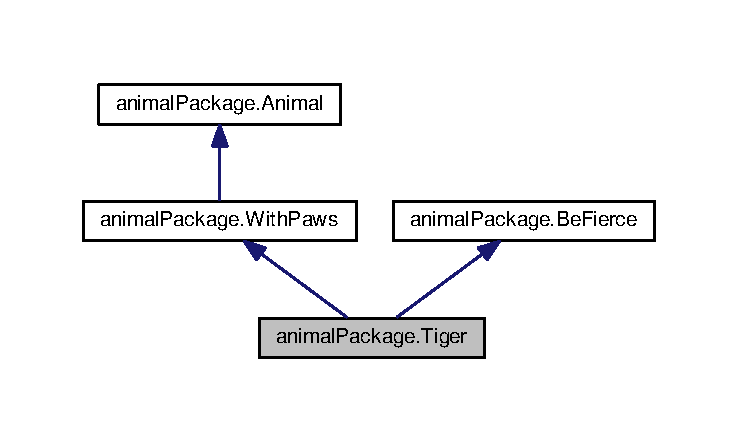
\includegraphics[width=350pt]{classanimal_package_1_1_tiger__inherit__graph}
\end{center}
\end{figure}


Collaboration diagram for animal\+Package.\+Tiger\+:\nopagebreak
\begin{figure}[H]
\begin{center}
\leavevmode
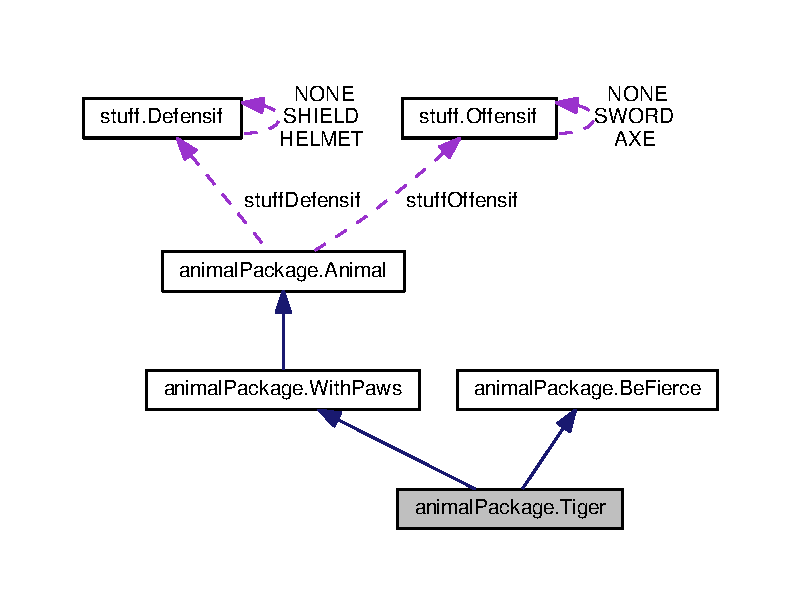
\includegraphics[width=350pt]{classanimal_package_1_1_tiger__coll__graph}
\end{center}
\end{figure}
\subsection*{Public Member Functions}
\begin{DoxyCompactItemize}
\item 
\hyperlink{classanimal_package_1_1_tiger_abe8e89cf608f68913595987734122e10}{Tiger} (String new\+Pseudo)
\item 
\hyperlink{classanimal_package_1_1_tiger_afa1cdc462c70c51b4cb98f5b3e917cb2}{Tiger} (String new\+Pseudo, String new\+Color)
\item 
void \hyperlink{classanimal_package_1_1_tiger_a977dc38b64fd5cfcd4e2ae3de1961b9e}{attack} (\hyperlink{classanimal_package_1_1_animal}{Animal} attacked\+Animal)
\item 
String \hyperlink{classanimal_package_1_1_tiger_aad61b38dbdbd08c6901eeff28e0c4d34}{special\+Action} (\hyperlink{classanimal_package_1_1_animal}{Animal} attacked\+Animal)
\item 
void \hyperlink{classanimal_package_1_1_tiger_a761264a91fd1bbe3684e70dbb4907fbd}{scream} ()
\item 
String \hyperlink{classanimal_package_1_1_tiger_a9c941af145fed9f1d71176ff6a752e16}{be\+Fierce} ()
\end{DoxyCompactItemize}
\subsection*{Additional Inherited Members}


\subsection{Detailed Description}
===== Class \hyperlink{classanimal_package_1_1_tiger}{Tiger} =====

\begin{DoxyAuthor}{Author}
Vincent Reynaert, Nicolas Sobczak 
\end{DoxyAuthor}
\begin{DoxyVersion}{Version}
1.\+03, 11/2016 
\end{DoxyVersion}


\subsection{Constructor \& Destructor Documentation}
\index{animal\+Package\+::\+Tiger@{animal\+Package\+::\+Tiger}!Tiger@{Tiger}}
\index{Tiger@{Tiger}!animal\+Package\+::\+Tiger@{animal\+Package\+::\+Tiger}}
\subsubsection[{\texorpdfstring{Tiger(\+String new\+Pseudo)}{Tiger(String newPseudo)}}]{\setlength{\rightskip}{0pt plus 5cm}animal\+Package.\+Tiger.\+Tiger (
\begin{DoxyParamCaption}
\item[{String}]{new\+Pseudo}
\end{DoxyParamCaption}
)}\hypertarget{classanimal_package_1_1_tiger_abe8e89cf608f68913595987734122e10}{}\label{classanimal_package_1_1_tiger_abe8e89cf608f68913595987734122e10}
Constructor


\begin{DoxyParams}{Parameters}
{\em 1} & String = tiger\textquotesingle{}s Pseudo \\
\hline
\end{DoxyParams}
\index{animal\+Package\+::\+Tiger@{animal\+Package\+::\+Tiger}!Tiger@{Tiger}}
\index{Tiger@{Tiger}!animal\+Package\+::\+Tiger@{animal\+Package\+::\+Tiger}}
\subsubsection[{\texorpdfstring{Tiger(\+String new\+Pseudo, String new\+Color)}{Tiger(String newPseudo, String newColor)}}]{\setlength{\rightskip}{0pt plus 5cm}animal\+Package.\+Tiger.\+Tiger (
\begin{DoxyParamCaption}
\item[{String}]{new\+Pseudo, }
\item[{String}]{new\+Color}
\end{DoxyParamCaption}
)}\hypertarget{classanimal_package_1_1_tiger_afa1cdc462c70c51b4cb98f5b3e917cb2}{}\label{classanimal_package_1_1_tiger_afa1cdc462c70c51b4cb98f5b3e917cb2}
Constructor


\begin{DoxyParams}{Parameters}
{\em 1} & String = tiger\textquotesingle{}s Pseudo \\
\hline
{\em 1} & String = tiger\textquotesingle{}s color \\
\hline
\end{DoxyParams}


\subsection{Member Function Documentation}
\index{animal\+Package\+::\+Tiger@{animal\+Package\+::\+Tiger}!attack@{attack}}
\index{attack@{attack}!animal\+Package\+::\+Tiger@{animal\+Package\+::\+Tiger}}
\subsubsection[{\texorpdfstring{attack(\+Animal attacked\+Animal)}{attack(Animal attackedAnimal)}}]{\setlength{\rightskip}{0pt plus 5cm}void animal\+Package.\+Tiger.\+attack (
\begin{DoxyParamCaption}
\item[{{\bf Animal}}]{attacked\+Animal}
\end{DoxyParamCaption}
)}\hypertarget{classanimal_package_1_1_tiger_a977dc38b64fd5cfcd4e2ae3de1961b9e}{}\label{classanimal_package_1_1_tiger_a977dc38b64fd5cfcd4e2ae3de1961b9e}
attack \+: function which executes a basic attack


\begin{DoxyParams}{Parameters}
{\em \hyperlink{classanimal_package_1_1_animal}{Animal}} & attacked\+Animal \\
\hline
\end{DoxyParams}
\index{animal\+Package\+::\+Tiger@{animal\+Package\+::\+Tiger}!be\+Fierce@{be\+Fierce}}
\index{be\+Fierce@{be\+Fierce}!animal\+Package\+::\+Tiger@{animal\+Package\+::\+Tiger}}
\subsubsection[{\texorpdfstring{be\+Fierce()}{beFierce()}}]{\setlength{\rightskip}{0pt plus 5cm}String animal\+Package.\+Tiger.\+be\+Fierce (
\begin{DoxyParamCaption}
{}
\end{DoxyParamCaption}
)}\hypertarget{classanimal_package_1_1_tiger_a9c941af145fed9f1d71176ff6a752e16}{}\label{classanimal_package_1_1_tiger_a9c941af145fed9f1d71176ff6a752e16}
be\+Fierce \+: function which return an adjective to describe behavior

\begin{DoxyReturn}{Returns}
1 String = an adjective 
\end{DoxyReturn}


Implements \hyperlink{interfaceanimal_package_1_1_be_fierce_aaa3925a8d59cbeccc2cb2a6d46d4ba2e}{animal\+Package.\+Be\+Fierce}.

\index{animal\+Package\+::\+Tiger@{animal\+Package\+::\+Tiger}!scream@{scream}}
\index{scream@{scream}!animal\+Package\+::\+Tiger@{animal\+Package\+::\+Tiger}}
\subsubsection[{\texorpdfstring{scream()}{scream()}}]{\setlength{\rightskip}{0pt plus 5cm}void animal\+Package.\+Tiger.\+scream (
\begin{DoxyParamCaption}
{}
\end{DoxyParamCaption}
)}\hypertarget{classanimal_package_1_1_tiger_a761264a91fd1bbe3684e70dbb4907fbd}{}\label{classanimal_package_1_1_tiger_a761264a91fd1bbe3684e70dbb4907fbd}
scream \+: function which makes the animal scream \index{animal\+Package\+::\+Tiger@{animal\+Package\+::\+Tiger}!special\+Action@{special\+Action}}
\index{special\+Action@{special\+Action}!animal\+Package\+::\+Tiger@{animal\+Package\+::\+Tiger}}
\subsubsection[{\texorpdfstring{special\+Action(\+Animal attacked\+Animal)}{specialAction(Animal attackedAnimal)}}]{\setlength{\rightskip}{0pt plus 5cm}String animal\+Package.\+Tiger.\+special\+Action (
\begin{DoxyParamCaption}
\item[{{\bf Animal}}]{attacked\+Animal}
\end{DoxyParamCaption}
)}\hypertarget{classanimal_package_1_1_tiger_aad61b38dbdbd08c6901eeff28e0c4d34}{}\label{classanimal_package_1_1_tiger_aad61b38dbdbd08c6901eeff28e0c4d34}
special\+Action \+: function which executes a special attack


\begin{DoxyParams}{Parameters}
{\em \hyperlink{classanimal_package_1_1_animal}{Animal}} & attacked\+Animal \\
\hline
\end{DoxyParams}
\begin{DoxyReturn}{Returns}
String 
\end{DoxyReturn}


The documentation for this class was generated from the following file\+:\begin{DoxyCompactItemize}
\item 
src/animal\+Package/Tiger.\+java\end{DoxyCompactItemize}

\hypertarget{classspace_objects_1_1_ufo}{}\section{space\+Objects.\+Ufo Class Reference}
\label{classspace_objects_1_1_ufo}\index{space\+Objects.\+Ufo@{space\+Objects.\+Ufo}}


Inheritance diagram for space\+Objects.\+Ufo\+:\nopagebreak
\begin{figure}[H]
\begin{center}
\leavevmode
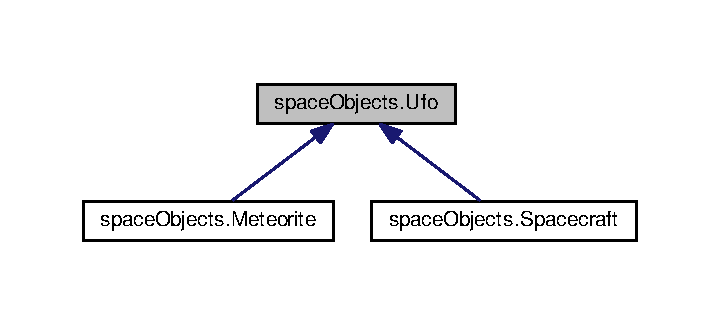
\includegraphics[width=346pt]{classspace_objects_1_1_ufo__inherit__graph}
\end{center}
\end{figure}
\subsection*{Public Member Functions}
\begin{DoxyCompactItemize}
\item 
\hyperlink{classspace_objects_1_1_ufo_a5dcb832d2c79687ffa2c199b320a8f3f}{Ufo} ()
\item 
\hyperlink{classspace_objects_1_1_ufo_af47b20fc2f0854016bd5685fe5a7177b}{Ufo} (\hyperlink{enumspace_objects_1_1_positions_cube}{Positions\+Cube} position)
\item 
\hyperlink{enumspace_objects_1_1_positions_cube}{Positions\+Cube} \hyperlink{classspace_objects_1_1_ufo_a28845916a0aab8e44687a4e2a3df45c7}{get\+Location} ()
\item 
void \hyperlink{classspace_objects_1_1_ufo_a240e9f0d9ad75cf0ebe650dd95564cb1}{set\+Location} (\hyperlink{enumspace_objects_1_1_positions_cube}{Positions\+Cube} position)
\item 
void \hyperlink{classspace_objects_1_1_ufo_a1dc5bd9259b652bac4cc0d97949b6274}{set\+Location} (int position)  throws Position\+Exception 
\end{DoxyCompactItemize}


\subsection{Detailed Description}
===== Class \hyperlink{classspace_objects_1_1_ufo}{Ufo} =====

useful to have position in the cube

\begin{DoxyAuthor}{Author}
Vincent Reynaert, Nicolas Sobczak 
\end{DoxyAuthor}
\begin{DoxyVersion}{Version}
1.\+02, 10/2016 
\end{DoxyVersion}


\subsection{Constructor \& Destructor Documentation}
\index{space\+Objects\+::\+Ufo@{space\+Objects\+::\+Ufo}!Ufo@{Ufo}}
\index{Ufo@{Ufo}!space\+Objects\+::\+Ufo@{space\+Objects\+::\+Ufo}}
\subsubsection[{\texorpdfstring{Ufo()}{Ufo()}}]{\setlength{\rightskip}{0pt plus 5cm}space\+Objects.\+Ufo.\+Ufo (
\begin{DoxyParamCaption}
{}
\end{DoxyParamCaption}
)}\hypertarget{classspace_objects_1_1_ufo_a5dcb832d2c79687ffa2c199b320a8f3f}{}\label{classspace_objects_1_1_ufo_a5dcb832d2c79687ffa2c199b320a8f3f}
Constructor. Set location by default to (0,0,0) \index{space\+Objects\+::\+Ufo@{space\+Objects\+::\+Ufo}!Ufo@{Ufo}}
\index{Ufo@{Ufo}!space\+Objects\+::\+Ufo@{space\+Objects\+::\+Ufo}}
\subsubsection[{\texorpdfstring{Ufo(\+Positions\+Cube position)}{Ufo(PositionsCube position)}}]{\setlength{\rightskip}{0pt plus 5cm}space\+Objects.\+Ufo.\+Ufo (
\begin{DoxyParamCaption}
\item[{{\bf Positions\+Cube}}]{position}
\end{DoxyParamCaption}
)}\hypertarget{classspace_objects_1_1_ufo_af47b20fc2f0854016bd5685fe5a7177b}{}\label{classspace_objects_1_1_ufo_af47b20fc2f0854016bd5685fe5a7177b}
Constructor. with selected position


\begin{DoxyParams}{Parameters}
{\em 1} & \hyperlink{enumspace_objects_1_1_positions_cube}{Positions\+Cube} = position \\
\hline
\end{DoxyParams}


\subsection{Member Function Documentation}
\index{space\+Objects\+::\+Ufo@{space\+Objects\+::\+Ufo}!get\+Location@{get\+Location}}
\index{get\+Location@{get\+Location}!space\+Objects\+::\+Ufo@{space\+Objects\+::\+Ufo}}
\subsubsection[{\texorpdfstring{get\+Location()}{getLocation()}}]{\setlength{\rightskip}{0pt plus 5cm}{\bf Positions\+Cube} space\+Objects.\+Ufo.\+get\+Location (
\begin{DoxyParamCaption}
{}
\end{DoxyParamCaption}
)}\hypertarget{classspace_objects_1_1_ufo_a28845916a0aab8e44687a4e2a3df45c7}{}\label{classspace_objects_1_1_ufo_a28845916a0aab8e44687a4e2a3df45c7}
Get the \hyperlink{classspace_objects_1_1_ufo}{Ufo} location

\begin{DoxyReturn}{Returns}
1 Positions = location 
\end{DoxyReturn}
\index{space\+Objects\+::\+Ufo@{space\+Objects\+::\+Ufo}!set\+Location@{set\+Location}}
\index{set\+Location@{set\+Location}!space\+Objects\+::\+Ufo@{space\+Objects\+::\+Ufo}}
\subsubsection[{\texorpdfstring{set\+Location(\+Positions\+Cube position)}{setLocation(PositionsCube position)}}]{\setlength{\rightskip}{0pt plus 5cm}void space\+Objects.\+Ufo.\+set\+Location (
\begin{DoxyParamCaption}
\item[{{\bf Positions\+Cube}}]{position}
\end{DoxyParamCaption}
)}\hypertarget{classspace_objects_1_1_ufo_a240e9f0d9ad75cf0ebe650dd95564cb1}{}\label{classspace_objects_1_1_ufo_a240e9f0d9ad75cf0ebe650dd95564cb1}
Set the \hyperlink{classspace_objects_1_1_ufo}{Ufo} location


\begin{DoxyParams}{Parameters}
{\em 1} & Postions\+Cube = position \\
\hline
\end{DoxyParams}
\index{space\+Objects\+::\+Ufo@{space\+Objects\+::\+Ufo}!set\+Location@{set\+Location}}
\index{set\+Location@{set\+Location}!space\+Objects\+::\+Ufo@{space\+Objects\+::\+Ufo}}
\subsubsection[{\texorpdfstring{set\+Location(int position)}{setLocation(int position)}}]{\setlength{\rightskip}{0pt plus 5cm}void space\+Objects.\+Ufo.\+set\+Location (
\begin{DoxyParamCaption}
\item[{int}]{position}
\end{DoxyParamCaption}
) throws {\bf Position\+Exception}}\hypertarget{classspace_objects_1_1_ufo_a1dc5bd9259b652bac4cc0d97949b6274}{}\label{classspace_objects_1_1_ufo_a1dc5bd9259b652bac4cc0d97949b6274}
Set the \hyperlink{classspace_objects_1_1_ufo}{Ufo} location


\begin{DoxyParams}{Parameters}
{\em 1} & int = position \\
\hline
\end{DoxyParams}


The documentation for this class was generated from the following file\+:\begin{DoxyCompactItemize}
\item 
src/space\+Objects/Ufo.\+java\end{DoxyCompactItemize}

\hypertarget{classanimal_package_1_1_with_paws}{}\section{animal\+Package.\+With\+Paws Class Reference}
\label{classanimal_package_1_1_with_paws}\index{animal\+Package.\+With\+Paws@{animal\+Package.\+With\+Paws}}


Inheritance diagram for animal\+Package.\+With\+Paws\+:\nopagebreak
\begin{figure}[H]
\begin{center}
\leavevmode
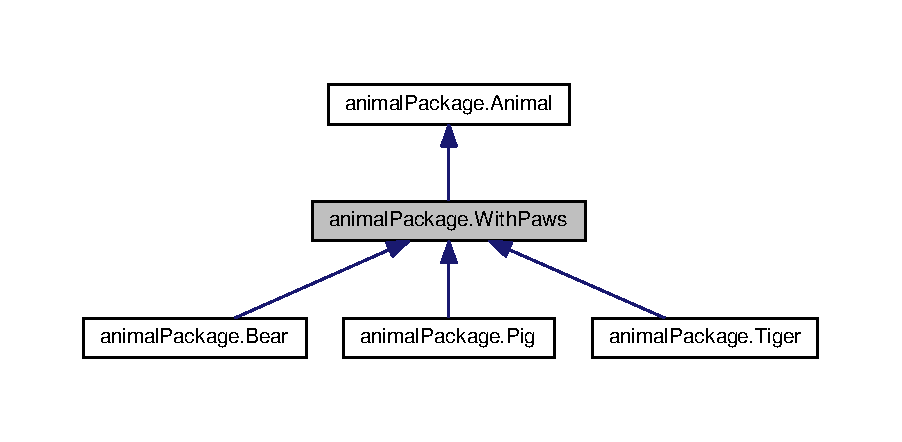
\includegraphics[width=350pt]{classanimal_package_1_1_with_paws__inherit__graph}
\end{center}
\end{figure}


Collaboration diagram for animal\+Package.\+With\+Paws\+:\nopagebreak
\begin{figure}[H]
\begin{center}
\leavevmode
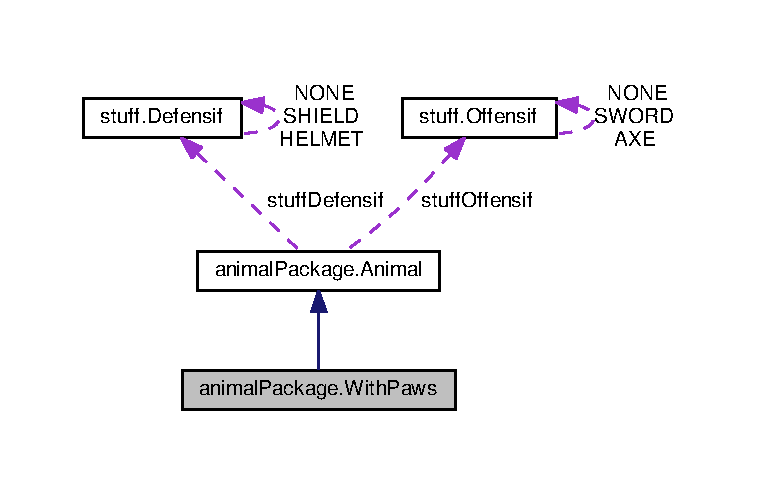
\includegraphics[width=350pt]{classanimal_package_1_1_with_paws__coll__graph}
\end{center}
\end{figure}
\subsection*{Public Member Functions}
\begin{DoxyCompactItemize}
\item 
\hyperlink{classanimal_package_1_1_with_paws_abc08a140d51063f3177e8c68d1e2e07e}{With\+Paws} (String new\+Pseudo)
\item 
\hyperlink{classanimal_package_1_1_with_paws_abf910b85727ade2a10742821068655fe}{With\+Paws} (String new\+Pseudo, String new\+Color)
\item 
void \hyperlink{classanimal_package_1_1_with_paws_a43a1d928b025e6dd40196ea31e8f4283}{attack} (\hyperlink{classanimal_package_1_1_animal}{Animal} attacked\+Animal)
\item 
String \hyperlink{classanimal_package_1_1_with_paws_a99f083a26533cfefae9134011b1c6a23}{special\+Action} (\hyperlink{classanimal_package_1_1_animal}{Animal} attacked\+Animal)
\end{DoxyCompactItemize}
\subsection*{Additional Inherited Members}


\subsection{Detailed Description}
===== Abstract Class \hyperlink{classanimal_package_1_1_with_paws}{With\+Paws} =====

\begin{DoxyAuthor}{Author}
Vincent Reynaert, Nicolas Sobczak 
\end{DoxyAuthor}
\begin{DoxyVersion}{Version}
1.\+03, 11/2016 
\end{DoxyVersion}


\subsection{Constructor \& Destructor Documentation}
\index{animal\+Package\+::\+With\+Paws@{animal\+Package\+::\+With\+Paws}!With\+Paws@{With\+Paws}}
\index{With\+Paws@{With\+Paws}!animal\+Package\+::\+With\+Paws@{animal\+Package\+::\+With\+Paws}}
\subsubsection[{\texorpdfstring{With\+Paws(\+String new\+Pseudo)}{WithPaws(String newPseudo)}}]{\setlength{\rightskip}{0pt plus 5cm}animal\+Package.\+With\+Paws.\+With\+Paws (
\begin{DoxyParamCaption}
\item[{String}]{new\+Pseudo}
\end{DoxyParamCaption}
)}\hypertarget{classanimal_package_1_1_with_paws_abc08a140d51063f3177e8c68d1e2e07e}{}\label{classanimal_package_1_1_with_paws_abc08a140d51063f3177e8c68d1e2e07e}
Constructor


\begin{DoxyParams}{Parameters}
{\em 1} & String = animal\textquotesingle{}s Pseudo \\
\hline
\end{DoxyParams}
\index{animal\+Package\+::\+With\+Paws@{animal\+Package\+::\+With\+Paws}!With\+Paws@{With\+Paws}}
\index{With\+Paws@{With\+Paws}!animal\+Package\+::\+With\+Paws@{animal\+Package\+::\+With\+Paws}}
\subsubsection[{\texorpdfstring{With\+Paws(\+String new\+Pseudo, String new\+Color)}{WithPaws(String newPseudo, String newColor)}}]{\setlength{\rightskip}{0pt plus 5cm}animal\+Package.\+With\+Paws.\+With\+Paws (
\begin{DoxyParamCaption}
\item[{String}]{new\+Pseudo, }
\item[{String}]{new\+Color}
\end{DoxyParamCaption}
)}\hypertarget{classanimal_package_1_1_with_paws_abf910b85727ade2a10742821068655fe}{}\label{classanimal_package_1_1_with_paws_abf910b85727ade2a10742821068655fe}
Constructor


\begin{DoxyParams}{Parameters}
{\em 1} & String = animal\textquotesingle{}s Pseudo \\
\hline
{\em 1} & String = animal\textquotesingle{}s color \\
\hline
\end{DoxyParams}


\subsection{Member Function Documentation}
\index{animal\+Package\+::\+With\+Paws@{animal\+Package\+::\+With\+Paws}!attack@{attack}}
\index{attack@{attack}!animal\+Package\+::\+With\+Paws@{animal\+Package\+::\+With\+Paws}}
\subsubsection[{\texorpdfstring{attack(\+Animal attacked\+Animal)}{attack(Animal attackedAnimal)}}]{\setlength{\rightskip}{0pt plus 5cm}void animal\+Package.\+With\+Paws.\+attack (
\begin{DoxyParamCaption}
\item[{{\bf Animal}}]{attacked\+Animal}
\end{DoxyParamCaption}
)}\hypertarget{classanimal_package_1_1_with_paws_a43a1d928b025e6dd40196ea31e8f4283}{}\label{classanimal_package_1_1_with_paws_a43a1d928b025e6dd40196ea31e8f4283}
attack \+: function which executes a basic attack


\begin{DoxyParams}{Parameters}
{\em \hyperlink{classanimal_package_1_1_animal}{Animal}} & attacked\+Animal \\
\hline
\end{DoxyParams}
\index{animal\+Package\+::\+With\+Paws@{animal\+Package\+::\+With\+Paws}!special\+Action@{special\+Action}}
\index{special\+Action@{special\+Action}!animal\+Package\+::\+With\+Paws@{animal\+Package\+::\+With\+Paws}}
\subsubsection[{\texorpdfstring{special\+Action(\+Animal attacked\+Animal)}{specialAction(Animal attackedAnimal)}}]{\setlength{\rightskip}{0pt plus 5cm}String animal\+Package.\+With\+Paws.\+special\+Action (
\begin{DoxyParamCaption}
\item[{{\bf Animal}}]{attacked\+Animal}
\end{DoxyParamCaption}
)}\hypertarget{classanimal_package_1_1_with_paws_a99f083a26533cfefae9134011b1c6a23}{}\label{classanimal_package_1_1_with_paws_a99f083a26533cfefae9134011b1c6a23}
attack \+: function which executes a special attack


\begin{DoxyParams}{Parameters}
{\em \hyperlink{classanimal_package_1_1_animal}{Animal}} & attacked\+Animal \\
\hline
\end{DoxyParams}


The documentation for this class was generated from the following file\+:\begin{DoxyCompactItemize}
\item 
src/animal\+Package/With\+Paws.\+java\end{DoxyCompactItemize}

\hypertarget{classanimal_package_1_1_with_wings}{}\section{animal\+Package.\+With\+Wings Class Reference}
\label{classanimal_package_1_1_with_wings}\index{animal\+Package.\+With\+Wings@{animal\+Package.\+With\+Wings}}


Inheritance diagram for animal\+Package.\+With\+Wings\+:\nopagebreak
\begin{figure}[H]
\begin{center}
\leavevmode
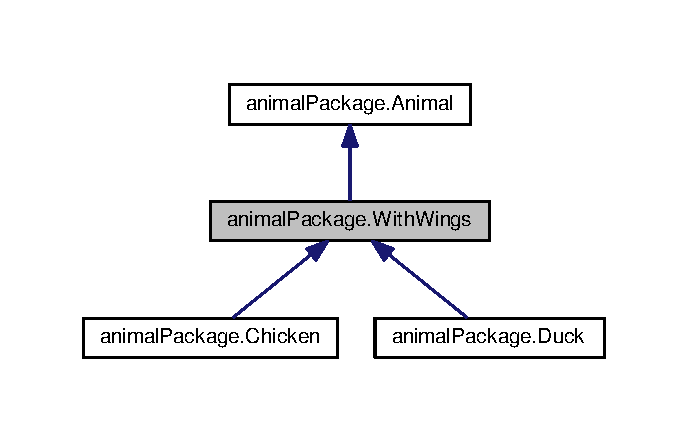
\includegraphics[width=330pt]{classanimal_package_1_1_with_wings__inherit__graph}
\end{center}
\end{figure}


Collaboration diagram for animal\+Package.\+With\+Wings\+:\nopagebreak
\begin{figure}[H]
\begin{center}
\leavevmode
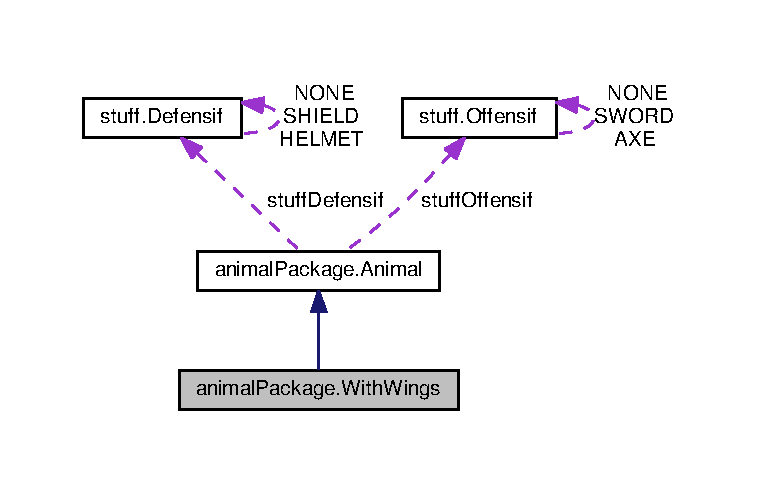
\includegraphics[width=350pt]{classanimal_package_1_1_with_wings__coll__graph}
\end{center}
\end{figure}
\subsection*{Public Member Functions}
\begin{DoxyCompactItemize}
\item 
\hyperlink{classanimal_package_1_1_with_wings_ac80503afecf307da50fbae841ab57270}{With\+Wings} (String new\+Pseudo)
\item 
\hyperlink{classanimal_package_1_1_with_wings_aa20719702326b6623b22b647a199cc9a}{With\+Wings} (String new\+Pseudo, String new\+Color)
\item 
void \hyperlink{classanimal_package_1_1_with_wings_ab8b3f96f10f0e694aeb4d03c5efebbdc}{attack} (\hyperlink{classanimal_package_1_1_animal}{Animal} attacked\+Animal)
\item 
String \hyperlink{classanimal_package_1_1_with_wings_ad9b0b04fe2c5a1a3d46e8b8344c58b79}{special\+Action} (\hyperlink{classanimal_package_1_1_animal}{Animal} attacked\+Animal)
\end{DoxyCompactItemize}
\subsection*{Additional Inherited Members}


\subsection{Detailed Description}
===== Class \hyperlink{classanimal_package_1_1_with_wings}{With\+Wings} =====

\begin{DoxyAuthor}{Author}
Vincent Reynaert, Nicolas Sobczak 
\end{DoxyAuthor}
\begin{DoxyVersion}{Version}
1.\+03, 11/2016 
\end{DoxyVersion}


\subsection{Constructor \& Destructor Documentation}
\index{animal\+Package\+::\+With\+Wings@{animal\+Package\+::\+With\+Wings}!With\+Wings@{With\+Wings}}
\index{With\+Wings@{With\+Wings}!animal\+Package\+::\+With\+Wings@{animal\+Package\+::\+With\+Wings}}
\subsubsection[{\texorpdfstring{With\+Wings(\+String new\+Pseudo)}{WithWings(String newPseudo)}}]{\setlength{\rightskip}{0pt plus 5cm}animal\+Package.\+With\+Wings.\+With\+Wings (
\begin{DoxyParamCaption}
\item[{String}]{new\+Pseudo}
\end{DoxyParamCaption}
)}\hypertarget{classanimal_package_1_1_with_wings_ac80503afecf307da50fbae841ab57270}{}\label{classanimal_package_1_1_with_wings_ac80503afecf307da50fbae841ab57270}
Constructor


\begin{DoxyParams}{Parameters}
{\em 1} & String = animal\textquotesingle{}s Pseudo \\
\hline
\end{DoxyParams}
\index{animal\+Package\+::\+With\+Wings@{animal\+Package\+::\+With\+Wings}!With\+Wings@{With\+Wings}}
\index{With\+Wings@{With\+Wings}!animal\+Package\+::\+With\+Wings@{animal\+Package\+::\+With\+Wings}}
\subsubsection[{\texorpdfstring{With\+Wings(\+String new\+Pseudo, String new\+Color)}{WithWings(String newPseudo, String newColor)}}]{\setlength{\rightskip}{0pt plus 5cm}animal\+Package.\+With\+Wings.\+With\+Wings (
\begin{DoxyParamCaption}
\item[{String}]{new\+Pseudo, }
\item[{String}]{new\+Color}
\end{DoxyParamCaption}
)}\hypertarget{classanimal_package_1_1_with_wings_aa20719702326b6623b22b647a199cc9a}{}\label{classanimal_package_1_1_with_wings_aa20719702326b6623b22b647a199cc9a}
Constructor


\begin{DoxyParams}{Parameters}
{\em 1} & String = animal\textquotesingle{}s Pseudo \\
\hline
{\em 1} & String = animal\textquotesingle{}s color \\
\hline
\end{DoxyParams}


\subsection{Member Function Documentation}
\index{animal\+Package\+::\+With\+Wings@{animal\+Package\+::\+With\+Wings}!attack@{attack}}
\index{attack@{attack}!animal\+Package\+::\+With\+Wings@{animal\+Package\+::\+With\+Wings}}
\subsubsection[{\texorpdfstring{attack(\+Animal attacked\+Animal)}{attack(Animal attackedAnimal)}}]{\setlength{\rightskip}{0pt plus 5cm}void animal\+Package.\+With\+Wings.\+attack (
\begin{DoxyParamCaption}
\item[{{\bf Animal}}]{attacked\+Animal}
\end{DoxyParamCaption}
)}\hypertarget{classanimal_package_1_1_with_wings_ab8b3f96f10f0e694aeb4d03c5efebbdc}{}\label{classanimal_package_1_1_with_wings_ab8b3f96f10f0e694aeb4d03c5efebbdc}
attack \+: function which executes a basic attack


\begin{DoxyParams}{Parameters}
{\em \hyperlink{classanimal_package_1_1_animal}{Animal}} & attacked\+Animal \\
\hline
\end{DoxyParams}
\index{animal\+Package\+::\+With\+Wings@{animal\+Package\+::\+With\+Wings}!special\+Action@{special\+Action}}
\index{special\+Action@{special\+Action}!animal\+Package\+::\+With\+Wings@{animal\+Package\+::\+With\+Wings}}
\subsubsection[{\texorpdfstring{special\+Action(\+Animal attacked\+Animal)}{specialAction(Animal attackedAnimal)}}]{\setlength{\rightskip}{0pt plus 5cm}String animal\+Package.\+With\+Wings.\+special\+Action (
\begin{DoxyParamCaption}
\item[{{\bf Animal}}]{attacked\+Animal}
\end{DoxyParamCaption}
)}\hypertarget{classanimal_package_1_1_with_wings_ad9b0b04fe2c5a1a3d46e8b8344c58b79}{}\label{classanimal_package_1_1_with_wings_ad9b0b04fe2c5a1a3d46e8b8344c58b79}
attack \+: function which executes a special attack


\begin{DoxyParams}{Parameters}
{\em \hyperlink{classanimal_package_1_1_animal}{Animal}} & attacked\+Animal \\
\hline
\end{DoxyParams}


The documentation for this class was generated from the following file\+:\begin{DoxyCompactItemize}
\item 
src/animal\+Package/With\+Wings.\+java\end{DoxyCompactItemize}

%--- End generated contents ---

% Index
\backmatter
\newpage
\phantomsection
\clearemptydoublepage
\addcontentsline{toc}{chapter}{Index}
\printindex

\end{document}
